% !TeX program = xelatex
\documentclass[11pt]{article}
\providecommand{\notesdir}{.}

% -----------------------------------------------------------------------------
% Shared preamble for the CO5059 topic notes, the final exam review and the
% cheat sheet's sibling documents.
% Documents outside this folder define \notesdir (path to this folder) first.
% -----------------------------------------------------------------------------

% Page layout and typography
\usepackage[a4paper,portrait,margin=1in]{geometry}
\usepackage{fontspec}
\usepackage{microtype}
\usepackage{parskip}
\setlength{\emergencystretch}{1.5em}% fewer overfull lines

% Mathematics and diagrams
\usepackage{amsmath,amssymb,amsthm,mathtools}
\usepackage{tikz-cd}
\usetikzlibrary{arrows.meta,positioning,shapes.geometric,shapes.arrows,
  shapes.multipart,calc,fit,backgrounds,matrix,patterns,decorations.pathreplacing}

% Reusable styles for flowcharts and concept diagrams.
\tikzset{
  concept/.style={
    draw=brandprimary,
    fill=brandsecondary!8,
    rounded corners,
    minimum width=3.2cm,
    minimum height=0.9cm,
    align=center,
    font=\small,
  },
  diagram arrow/.style={-{Latex[length=2.5mm]},thick,brandprimary},
  % tree nodes (e.g. Tree-LRU) and hardware blocks
  tnode/.style={draw,rectangle,font=\small\ttfamily,inner sep=3pt,
    minimum height=0.55cm,fill=white},
  box/.style={draw,rectangle,align=center,font=\small,inner sep=4pt,
    fill=white},
  % ALU drawn vertically (inputs on the top edge, output at the bottom):
  % \pic at (x,y) {valu}; inputs at (x-0.65,y), (x+0.65,y); output (x,y-1)
  valu/.pic={\draw[fill=white] (-1.1,0)--(-0.2,0)--(0,-0.3)--(0.2,0)--(1.1,0)
    --(0.5,-1)--(-0.5,-1)--cycle; \node[font=\scriptsize] at (0,-0.62) {ALU};},
}

% Tables, figures, code, and lists
\usepackage{graphicx}
\graphicspath{{\notesdir/}}
\usepackage{enumitem}
\usepackage{booktabs}
% array is pinned: a newer array.sty in the local texmf tree needs a newer
% LaTeX kernel than the installed one; the dated rollback works with both.
\usepackage{array}[=2024-06-01]
% P{w}: paragraph column set ragged right (no stretched word gaps in tables)
\newcolumntype{P}[1]{>{\raggedright\arraybackslash}p{#1}}
\usepackage{listings}

% Color and links
\usepackage[dvipsnames]{xcolor}
% Same palette as the other course notes (co5115):
% brandprimary = navy lines/arrows/links, brandsecondary!NN = light blue fills.
\definecolor{brandprimary}{HTML}{030391}
\definecolor{brandsecondary}{HTML}{1488D8}
\usepackage[
  colorlinks=true,
  linkcolor=brandprimary,
  citecolor=brandsecondary,
  urlcolor=brandsecondary
]{hyperref}

% Headers and footers
\usepackage{fancyhdr}
\setlength{\headheight}{26pt}
\pagestyle{fancy}
\fancyhf{}
\fancyhead[L]{\small\textbf{\coursecode}\\\coursename}
\fancyhead[R]{\small HCMUT}
\fancyfoot[L]{\small Semester \semester}
\fancyfoot[R]{\small Page \thepage}

% -----------------------------------------------------------------------------
% Course information -- change these values once per course
% -----------------------------------------------------------------------------
\newcommand{\universityname}{HCMC University of Technology}
\newcommand{\faculty}{Faculty of Computer Science and Engineering}
\newcommand{\coursecode}{CO5059}
\newcommand{\coursename}{Advanced System Architectures}
\newcommand{\semester}{261}
\newcommand{\instructor}{Assoc.\ Prof.\ Tran Ngoc Thinh}
\newcommand{\instructoremail}{}% leave empty to hide
\newcommand{\notetaker}{Phan Nhat Minh}
\newcommand{\notetakeremail}{minh.phannhat95@hcmut.edu.vn}
\newcommand{\emaillink}[1]{%
  \href{mailto:#1}{\textcolor{brandprimary}{\texttt{#1}}}}

% Definitions, results, examples, proofs and notes in coloured boxes.
\input{\notesdir/colored-boxes}

% -----------------------------------------------------------------------------
% Course-specific notation
% -----------------------------------------------------------------------------
\newcommand{\CPI}{\mathrm{CPI}}
\newcommand{\AMAT}{\mathrm{AMAT}}

\lstdefinestyle{plain}{
  basicstyle=\ttfamily\small,
  showstringspaces=false,
  columns=fullflexible,
  keepspaces=true,
  breaklines=true,
  frame=single,
  framerule=0.3pt,
  rulecolor=\color{black!30},
  xleftmargin=4pt,
  xrightmargin=4pt,
}
\lstdefinestyle{mips}{
  style=plain,
  keywordstyle=\bfseries,
  morekeywords={lw,sw,add,sub,and,or,slt,beq,bne,beqz,xor,nop,addi,addiu,addu,
    subu,li,la,jal,jr,jalr,sll,srl,sra,sllv,srlv,srav,andi,ori,xori,nor,slti,
    sltiu,sltu,lui,mult,multu,div,divu,mfhi,mflo,ll,sc,syscall,move,lh,lhu,lb,
    lbu,sh,sb,blez,bgtz,bltz,bgez,j,mul,ld,sd,dadd,daddu,daddi,daddui,dsub,
    dsubu,bnez,l.d,s.d,add.d,sub.d,mul.d,div.d},
}
\lstset{style=mips}

% Long identifiers (GRADE_REPORT.Section_identifier) may break after "_".
\makeatletter
\DeclareRobustCommand{\_}{\ifmmode\nfss@text{\textunderscore}\else
  \textunderscore\allowbreak\fi}
\makeatother

% Marks a correction of an error in the slides: \begin{remark}\slidefix{} ...
\newcommand{\slidefix}{\textbf{\textcolor{red!75!black}{Slide correction.}}}
% Marks material added from the textbook or papers, not in the slides.
\newcommand{\beyond}{\textbf{Beyond the slides.}}

% -----------------------------------------------------------------------------
% Textbook citations as footnotes (book page + PDF page of textbooks/*.pdf)
% -----------------------------------------------------------------------------
% \srcnote{text}: a footnote that also works inside the coloured boxes
% (mdframed/tcolorbox would otherwise keep it inside the box with a letter).
% In a box it prints the mark and queues the text; the queue is emptied after
% the box (hooks below), so the note lands at the foot of the page.
\makeatletter
\newtoks\srcnote@pending
\def\srcnote@mp{mpfootnote}
\newcommand{\srcnote}[1]{%
  \ifx\@mpfn\srcnote@mp
    \stepcounter{footnote}%
    \protected@xdef\@thefnmark{\thefootnote}%
    \@footnotemark
    \xdef\srcnote@n{\the\c@footnote}%
    \global\srcnote@pending\expandafter{\the\expandafter\srcnote@pending
      \expandafter\footnotetext\expandafter[\srcnote@n]{#1}}%
  \else\footnote{#1}\fi}
\newcommand{\srcnote@flush}{\the\srcnote@pending\global\srcnote@pending{}}
\@for\srcnote@env:={theorem,definition,proposition,prop,lemma,corollary,%
exercise,tbexercise,example,eg,remark,note,solution,explanation,noot}\do{%
  \AddToHook{env/\srcnote@env/after}{\srcnote@flush}}
\makeatother
% Hennessy & Patterson, Computer Architecture: A Quantitative Approach, 5th ed.
% (references/Computer Architecture - A Quantitative Approach.pdf).
% Chapters: PDF page = printed page + 29.  Appendix X: page X-n is PDF n + offset.
\makeatletter
\@namedef{HPoff@}{29}
\@namedef{HPoff@A}{523}\@namedef{HPoff@B}{579}\@namedef{HPoff@C}{647}
\@namedef{HPoff@D}{736}\@namedef{HPoff@E}{804}\@namedef{HPoff@F}{831}
\@namedef{HPoff@G}{949}\@namedef{HPoff@H}{984}\@namedef{HPoff@I}{1029}
\@namedef{HPoff@J}{1076}\@namedef{HPoff@K}{1150}
% \hppage{X}{n}: "p. X-n (PDF p. m)"; X empty for a chapter page.
\newcommand{\hppage}[2]{p.~\if\relax\detokenize{#1}\relax\else#1-\fi#2\
  (PDF~\the\numexpr#2+\csname HPoff@#1\endcsname\relax)}
% \hppages{X}{first}{last}
\newcommand{\hppages}[3]{pp.~\if\relax\detokenize{#1}\relax\else#1-\fi#2--%
  \if\relax\detokenize{#1}\relax\else#1-\fi#3\
  (PDF~\the\numexpr#2+\csname HPoff@#1\endcsname\relax--%
  \the\numexpr#3+\csname HPoff@#1\endcsname\relax)}
\makeatother
% Footnote citations:
%   \HP{location}{page}            chapter page          \HP[last]{loc}{first}
%   \HPA{X}{location}{page}        appendix X page X-n   \HPA[last]{X}{loc}{first}
\newcommand{\HP}[3][]{\srcnote{H\&P 5th ed., #2,
  \if\relax\detokenize{#1}\relax\hppage{}{#3}\else\hppages{}{#3}{#1}\fi.}}
\newcommand{\HPA}[4][]{\srcnote{H\&P 5th ed., #3,
  \if\relax\detokenize{#1}\relax\hppage{#2}{#4}\else\hppages{#2}{#4}{#1}\fi.}}

% Textbook exercise. No solution is written: the box cites the exercise and
% the book pages with the theory needed to solve it.
% \begin{tbexercise}[appendix letter]{H&P number}{page}{theory pointer}
%   e.g. \begin{tbexercise}{1.8}{60}{\S1.9, \hppages{}{46}{48}}
%        \begin{tbexercise}[B]{B.1}{60}{\S B.2, \hppages{B}{15}{22}}
\makeatletter
\newenvironment{tbexercise}[4][]
  {\gdef\tbx@note{\srcnote{H\&P 5th ed., Exercise #2, \hppage{#1}{#3}.}}%
   \gdef\tbx@theory{#4}%
   \begin{exercise}[H\&P #2]}
  {\par\hfill{\small\itshape Theory: \tbx@theory}\tbx@note
   \end{exercise}}
\makeatother
% Source note under a diagram, for checking it against the original:
% \diagramsource{slides file, slide N; cf. textbook figure}
\newcounter{diagram}
% (the counter is stepped inside the note's line, so no page break can fall
% between the diagram and its note)
\newcommand{\diagramsource}[1]{\par\nopagebreak
  {\centering\footnotesize\itshape\color{black!65}\leavevmode\refstepcounter{diagram}%
   Diagram~\thediagram\ -- source: #1\par}}

% Source line under a section heading.
\newcommand{\sources}[1]{\par\noindent{\small\itshape\sloppy Sources: #1\par}\medskip}

% Cover page + contents page.  Usage: \makecover{Big title}
\newcommand{\makecover}[1]{%
\pagenumbering{roman}
\begin{titlepage}
  \thispagestyle{empty}
  \renewcommand{\emaillink}[1]{\href{mailto:##1}{\textcolor{black}{\texttt{##1}}}}% no colour on the cover

  \begin{center}
    
\includegraphics[width=0.62\textwidth]{assets/text_logo_3.png}

    \vspace{0.35cm}
    {\large\bfseries\faculty\par}
  \end{center}

  \vfill
  \begin{center}
    {\Huge\bfseries #1\par}
    \vspace{0.55cm}
    {\LARGE\bfseries\coursename\par}
    \vspace{0.2cm}
    {\large\coursecode\par}

    \vspace{0.65cm}
    \rule{0.38\textwidth}{0.6pt}
    \vspace{0.65cm}

    {\large\textbf{Instructor:} \instructor
      \ifx\instructoremail\empty\else\ {\small(\emaillink{\instructoremail})}\fi\par}
    \vspace{0.3cm}
    {\large\textbf{Notes by:} \notetaker\
      {\small(\emaillink{\notetakeremail})}\par}
    \vspace{0.3cm}
    {\large\textbf{Semester:} \semester\par}
  \end{center}

  \vfill
  \begin{center}
    \small Last updated: \today
  \end{center}
\end{titlepage}

% -----------------------------------------------------------------------------
% Table of contents -- kept on its own page
% -----------------------------------------------------------------------------
\clearpage
\setcounter{page}{2}
\thispagestyle{empty}
\hypersetup{linkcolor=black}
\setcounter{tocdepth}{2}
\tableofcontents
\hypersetup{linkcolor=brandprimary}
\clearpage
\pagenumbering{arabic}
}

% Every \section starts on a new page (notes only; the review shares the
% preamble but not this rule).
\AddToHook{cmd/section/before}{\clearpage}

\begin{document}
\makecover{Lecture Notes}

% -----------------------------------------------------------------------------
% Sections (one per topic, in course order)
% -----------------------------------------------------------------------------
\section{Introduction}
\label{sec:introduction}
\sources{Lecture ``Introduction'' (\nolinkurl{01-introduction-lecture.pdf});
H\&P 5th ed.\ Ch.~1 (Fundamentals of Quantitative Design and Analysis).}

\textbf{Computer architecture} is the design of the layers of a computer system
between the application and the transistors: the instruction set the software
sees, the organization of the processor and memory behind it, and the hardware
that implements them. An architect trades \emph{performance} against
\emph{cost}, within what technology allows.

\begin{center}\begin{minipage}{\linewidth}\centering
\begin{tikzpicture}[font=\small,
  topic/.style={concept,text width=3.4cm,minimum height=1.05cm}]
  \node[topic] (q) at (0,1.5) {\textbf{1 Introduction}\\performance, cost, Amdahl};
  \node[topic] (i) at (4.6,1.5) {\textbf{2 Instruction sets}\\ISA styles, MIPS};
  \node[topic] (p) at (9.2,1.5) {\textbf{3 Pipelining}\\stages, hazards};
  \node[topic] (c) at (0,0) {\textbf{4 Cache}\\organization, AMAT};
  \node[topic] (v) at (4.6,0) {\textbf{5 Virtual memory}\\paging, TLB};
  \node[topic] (m) at (9.2,0) {\textbf{6 Multiprocessors}\\ILP, TLP, coherence};
  \draw[diagram arrow] (q) -- (i);
  \draw[diagram arrow] (i) -- (p);
  \draw[diagram arrow] (c) -- (v);
  \draw[diagram arrow] (v) -- (m);
\end{tikzpicture}
\diagramsource{own diagram (roadmap of these notes); no source}
\end{minipage}
\end{center}

\paragraph{Roadmap.}
\begin{enumerate}
  \item \textbf{Introduction} (this section): technology trends
  (\S\ref{sec:architecture}), cost (\S\ref{sec:cost}), performance, the CPU
  equation and Amdahl's Law (\S\ref{sec:performance}), benchmarks
  (\S\ref{sec:benchmarking}).
  \item \textbf{Instruction set architecture} (Section~\ref{sec:isa}): ISA
  styles, addressing modes, encoding, CISC vs.\ RISC, and the MIPS case study
  (\S\ref{sec:mips}).
  \item \textbf{Pipelining} (Section~\ref{sec:pipelining}): the 5-stage MIPS
  pipeline, then structural, data and control hazards (\S\ref{sec:hazards}).
  \item \textbf{Cache} (Section~\ref{sec:cache}): organization, replacement,
  write policies, the 3 Cs, AMAT and multilevel caches, optimizations.
  \item \textbf{Virtual memory} (Section~\ref{sec:vm}): address translation,
  page tables, TLB, page replacement, segmentation, protection.
  \item \textbf{Multiprocessors} (Section~\ref{sec:mp}): Flynn's classes, UMA
  and NUMA, synchronization, memory consistency, ILP (superscalar, VLIW) and
  multithreading, cache coherence.
  \item \textbf{Practice problems} (Section~\ref{sec:practice}) and a
  \textbf{summary} (Section~\ref{sec:summary}).
\end{enumerate}

\paragraph{How the notes are built.} Lectures 1--3 were taught by the lecturer;
from cache on, the topics were presented by student groups and reviewed by the
lecturer. Group slides are checked against the textbook, J.~Hennessy and
D.~Patterson, \emph{Computer Architecture: A Quantitative Approach}, 5th ed.\
(H\&P). Footnotes give the book page and the PDF page of
\texttt{references/Computer Architecture - A Quantitative Approach.pdf}.
\slidefix{} in a remark marks a corrected slide error; \beyond{} marks material
added from the textbook. Each topic ends with selected textbook exercises; they
cite the exercise and the pages with the theory needed, without solutions.

\subsection{Computer Architecture and Technology Trends}
\label{sec:architecture}

\subsubsection{What Is Computer Architecture?}
\label{sec:what-is-architecture}

\paragraph{A changing definition}
\begin{itemize}
  \item \textbf{1950s--60s:} Computer Arithmetic.
  \item \textbf{1970s--mid-80s:} Instruction Set Design.
  \item \textbf{1990s:} Design of CPU, memory system, I/O system,
  multiprocessors, networks.
  \item \textbf{2000s:} Multi-core design, on-chip networking, parallel
  programming paradigms, power reduction.
  \item \textbf{2010s:} Low-power/mobile processing, self-adapting systems.
  \item \textbf{2020s:} AI chips, quantum computing.
\end{itemize}

\paragraph{Role of a computer architect}
\begin{definition}[Role of a computer architect]
To design and engineer the various levels of a computer system to
maximize \textbf{performance} and \textbf{programmability} within limits
of \textbf{technology} and \textbf{cost}.
\end{definition}

\paragraph{The task of the computer designer}
\begin{itemize}
  \item Determine what attributes are important for a new machine.
  \item Design a machine to maximize cost-performance.
  \item What are these tasks?
  \begin{itemize}
    \item Instruction set design
    \item Functional organization
    \item Logic design
    \item Implementation: IC design, packaging, power, cooling, \dots
  \end{itemize}
\end{itemize}

\paragraph{Levels of abstraction}

Software and hardware consist of hierarchical layers of abstraction, each
hiding the details of the layers below it from the layer above.

\begin{definition}[Instruction Set Architecture]
The \emph{Instruction Set Architecture} (ISA) is the layer that abstracts the
hardware/software interface. It allows many implementations of varying cost
and performance to run the same software.\HP[17]{\S1.3}{11}
\end{definition}

\begin{center}\begin{minipage}{\linewidth}\centering
\begin{tikzpicture}[x=1cm,y=0.62cm,font=\small]
  % software (above the ISA)
  \draw (0,1) rectangle (10,4.6);
  \node[anchor=north west] at (0.1,4.55) {Applications};
  \draw (3.4,1) rectangle (10,3.5);
  \node[anchor=north] at (6.7,3.45) {Operating System};
  \draw (4.0,1) rectangle (6.6,2.1) node[midway] {Compiler};
  \draw (7.0,1) rectangle (9.6,2.1) node[midway] {Firmware};
  % the interface
  \draw[fill=black!12,thick] (-0.4,0.25) rectangle (10.4,1) node[midway] {\bfseries Instruction Set Architecture};
  % hardware (below the ISA)
  \draw (0.4,-0.6) rectangle (6.4,0.25) node[midway] {Instruction Set Processor};
  \draw (6.4,-0.6) rectangle (9.6,0.25) node[midway] {I/O System};
  \draw (1.0,-1.45) rectangle (9.0,-0.6) node[midway] {Datapath \& Control};
  \draw (1.6,-2.3) rectangle (8.4,-1.45) node[midway] {Digital Design};
  \draw (2.2,-3.15) rectangle (7.8,-2.3) node[midway] {Circuit Design};
  \draw (2.8,-4.0) rectangle (7.2,-3.15) node[midway] {Layout};
  % side labels
  \draw[-{Latex[length=2.5mm]},thick] (-0.9,1.05) -- (-0.9,4.6)
    node[midway,rotate=90,above] {Software};
  \draw[-{Latex[length=2.5mm]},thick] (-0.9,0.2) -- (-0.9,-4.0)
    node[midway,rotate=90,above] {Hardware};
\end{tikzpicture}
\diagramsource{\nolinkurl{01-introduction-lecture.pdf}, slide 10 (``Levels of Abstraction''); redrawn}
\end{minipage}
\end{center}

\subsubsection{A Brief History}
\label{sec:brief-history}

\begin{itemize}
  \item \textbf{``Big Iron'' computers} (e.g.\ ENIAC 1945, IBM Mark~1 1944):
  used vacuum tubes, electric relays and bulk magnetic storage devices. No
  microprocessors, no (stored-program) memory.
  \item \textbf{Von Neumann}: invented EDSAC (1949), the first
  \emph{stored-program computer} -- uses memory to hold both instructions
  and data. \emph{We are still using this same basic design today.}
  \item \textbf{The processor chip}: the microprocessor evolution --
  Intel 4004 (1971) $\to$ 8086 (1978) $\to$ 80386 $\to$ 80486 $\to$
  Pentium $\to$ Pentium~II/III $\to \dots \to$ multi-core Core~i7, and
  today's Arrow~Lake / Panther~Lake (2026).
\end{itemize}

\paragraph{Selected microprocessor milestones (die data)}

\begin{center}
\begin{tabular}{@{}lrrrl@{}}
\toprule
Chip & Year & Transistors & Area & Notes \\
\midrule
Intel 4004      & 1970 & 2,250      & 12 mm$^2$  & first microprocessor, 108 KHz \\
Intel 8086      & 1979 & 29,000     & 33 mm$^2$  & 5 MHz; basis of IA32 PC \\
Intel 80486     & 1989 & 1,200,000  & 81 mm$^2$  & 25 MHz; 1st pipelined IA32 \\
Pentium         & 1993 & 3,100,000  & 296 mm$^2$ & 60 MHz; 1st superscalar IA32 \\
Pentium~III     & 1999 & 9,500,000  & 125 mm$^2$ & 450 MHz \\
\bottomrule
\end{tabular}
\end{center}

\paragraph{Intel x86 evolution: milestones}

\begin{center}
\begin{tabular}{@{}lrrrp{6cm}@{}}
\toprule
Name & Date & Transistors & MHz & Notes \\
\midrule
8086     & 1978 & 29K   & 5--10     & First 16-bit Intel processor; basis for IBM PC \& DOS; 1MB address space \\
386      & 1985 & 275K  & 16--33    & First 32-bit Intel processor (IA32); flat addressing, can run Unix \\
Pentium 4E & 2004 & 125M & 2800--3800 & First 64-bit Intel x86 processor (x86-64) \\
Core 2   & 2006 & 291M  & 1060--3333 & First multi-core Intel processor \\
Core i7  & 2008 & 731M  & 1600--4400 & Four cores \\
\bottomrule
\end{tabular}
\end{center}

\paragraph{Process technology}

\begin{center}
\begin{tabular}{@{}lr@{}}
\toprule
Generation & Process node \\
\midrule
1st Pentium Pro (1995) & 600 nm \\
1st Pentium III (1999) & 250 nm \\
1st Pentium 4 (2000)   & 180 nm \\
1st Core 2 Duo (2006)  & 65 nm \\
Nehalem (2008)         & 45 nm \\
Sandy Bridge (2011)    & 32 nm \\
Ivy/Haswell/Broadwell/Skylake/Kaby/Coffee Lake (2012--2017) & 22--14 nm \\
Ice/Tiger/Alder/Raptor Lake (2021--2023) & 10 nm \\
Meteor / Lunar Lake (2024) & 5--7 nm \\
Arrow Lake (2026)      & 3 nm \\
Panther Lake (2026)    & $\sim$2 nm (Intel 18A) \\
\bottomrule
\end{tabular}
\end{center}
Process technology dimension = width of narrowest wires (10 nm $\approx$ 100
atoms wide).

\paragraph{Moore's Law}
\begin{definition}[Moore's Law]
The number of transistors on a cost-effective integrated circuit doubles
every 18--24 months. (Gordon Moore, ``Cramming More Components onto
Integrated Circuits,'' \emph{Electronics}, 1965.)\HP[18]{\S1.4}{17}
\end{definition}
Transistor count has grown from a few thousand (1970s) to over 100 billion
transistors/chip today (e.g.\ Apple M2 Ultra, $\sim$134~billion).

\begin{center}\begin{minipage}{\linewidth}\centering
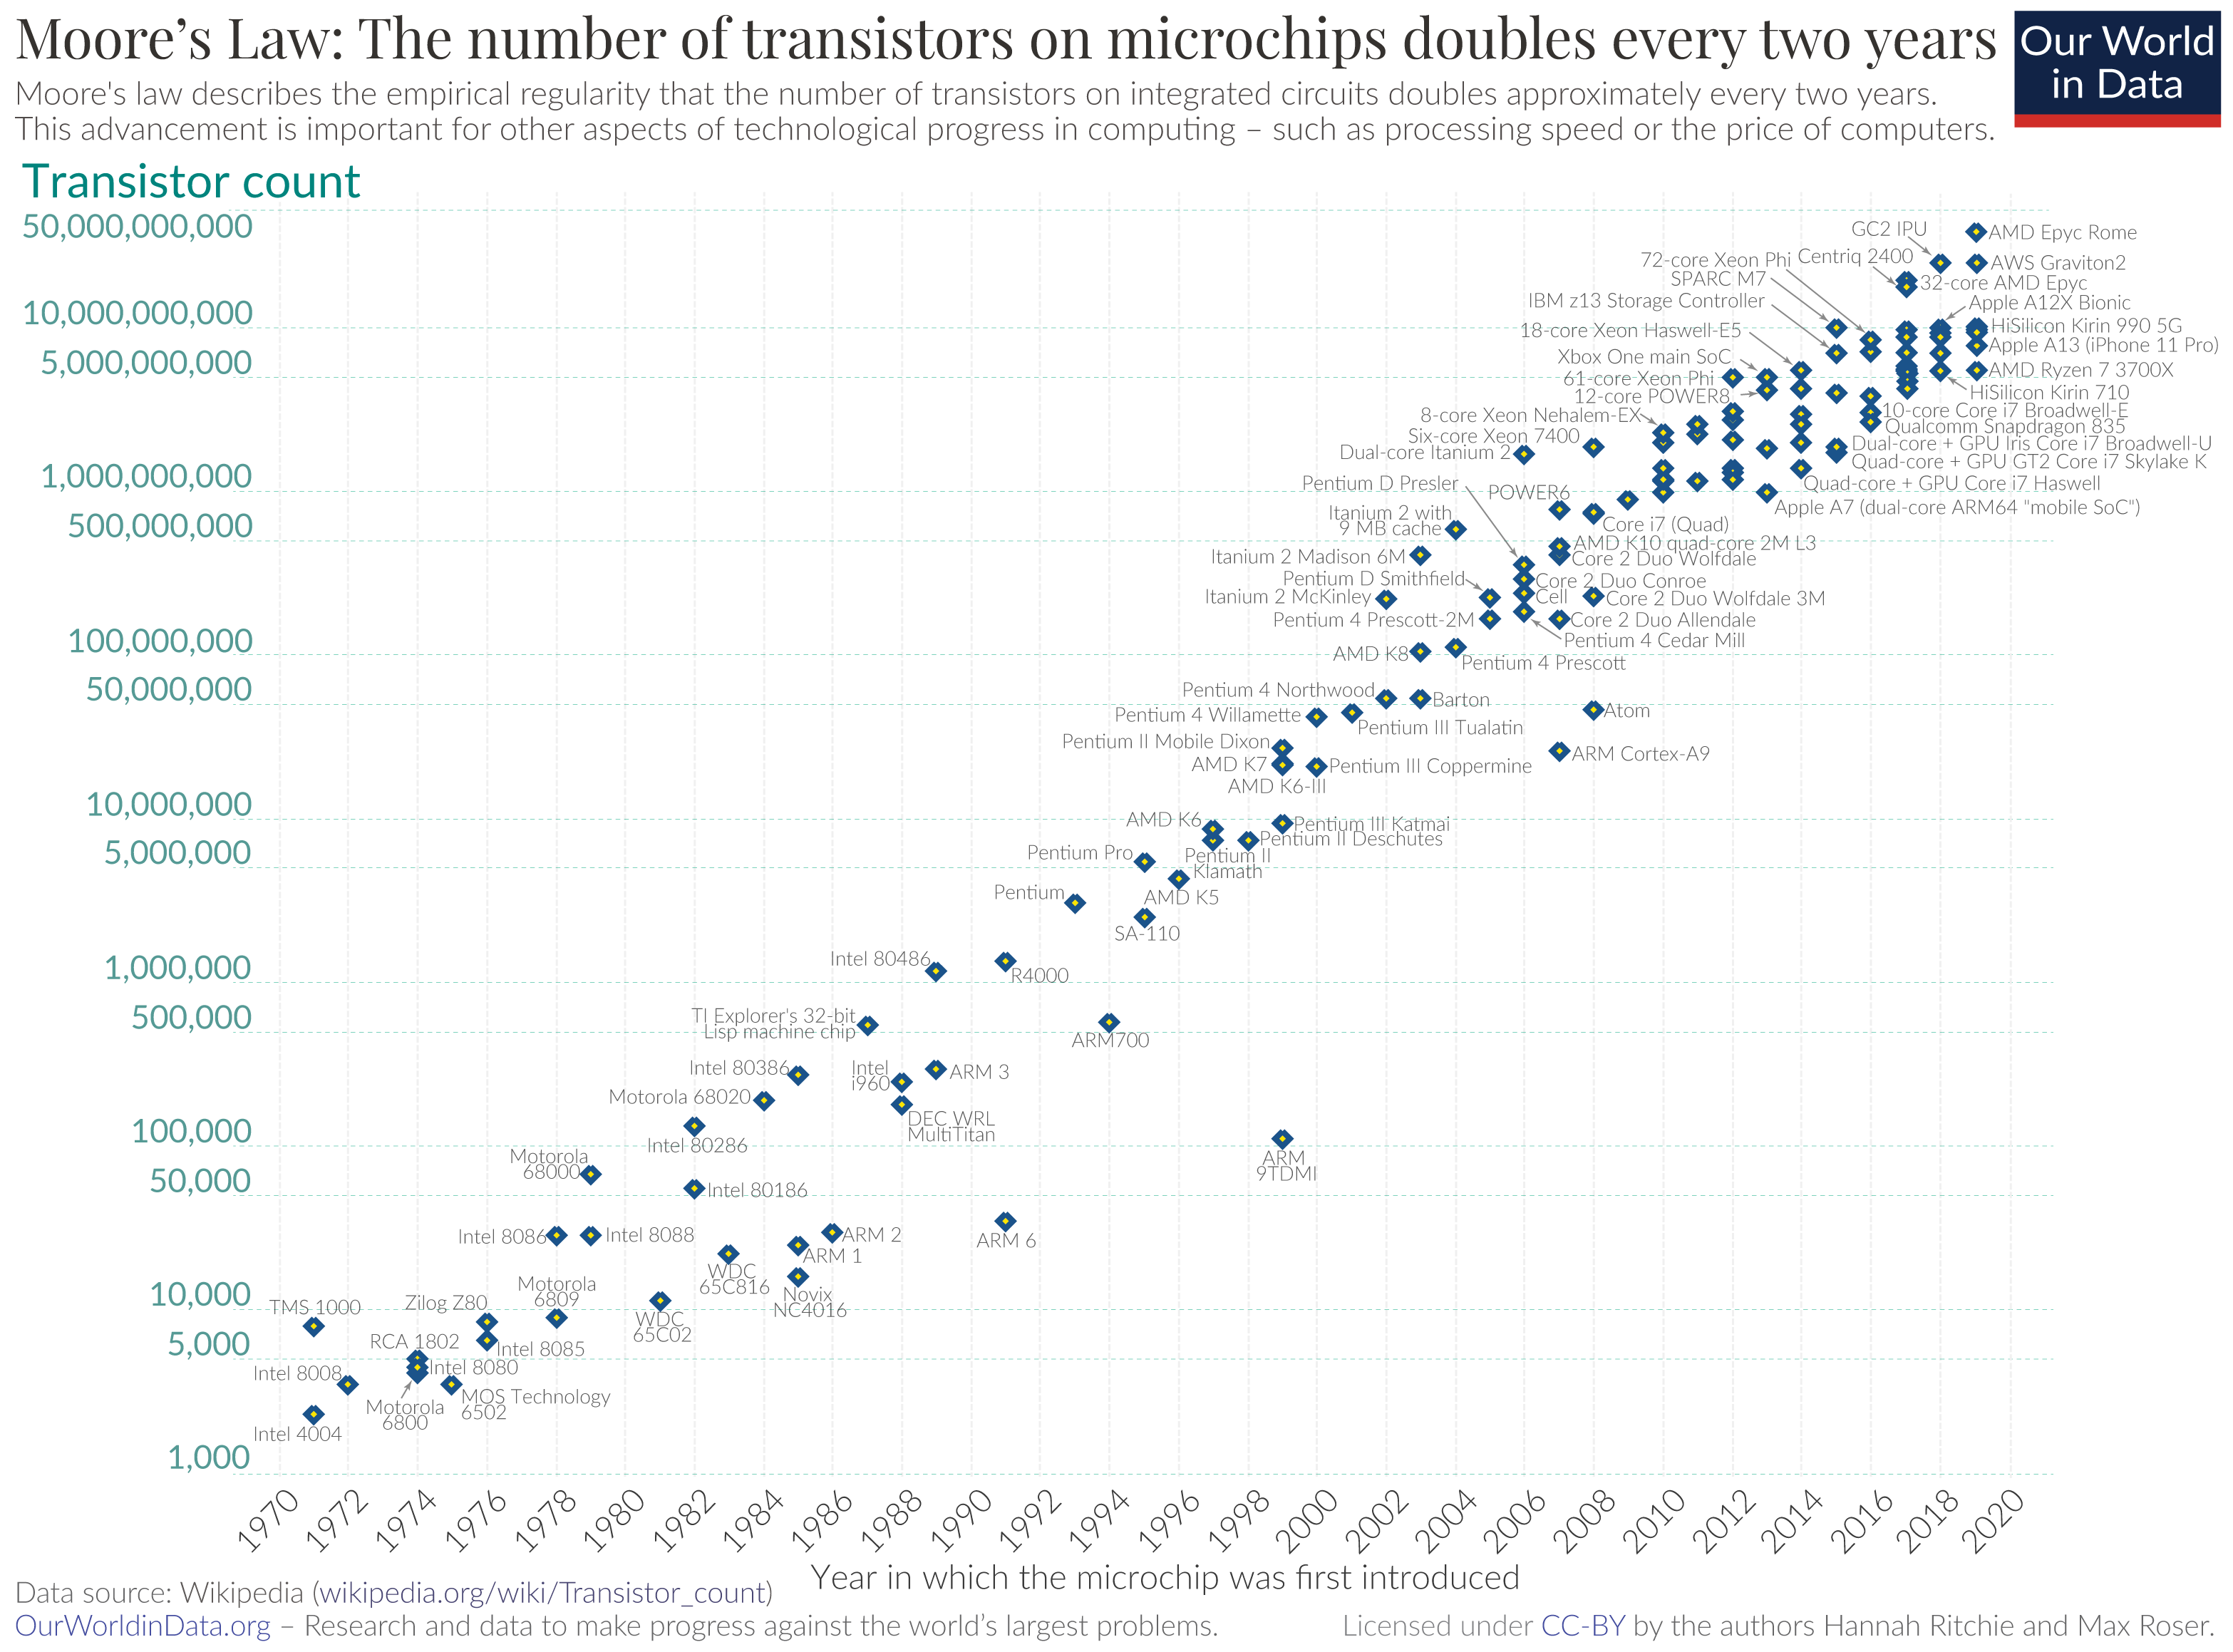
\includegraphics[width=0.92\linewidth]{assets/figures/moores-law-transistor-count-1970-2020.png}
\diagramsource{chart by Hannah Ritchie and Max Roser, Our World in Data, ``Moore's Law: The number of transistors on microchips doubles every two years'' (data: Wikipedia, licensed CC BY), \href{https://en.wikipedia.org/wiki/Moore\%27s_law\#/media/File:Moore's_Law_Transistor_Count_1970-2020.png}{Wikimedia Commons}; replaces the schematic of \nolinkurl{01-introduction-lecture.pdf}, slide 22 (``Moore's Law'')}
\end{minipage}
\end{center}

\paragraph{The end of the uniprocessor era}

\begin{itemize}
  \item ``\dots today's processors \dots are nearing an impasse as
  technologies approach the speed of light\dots'' -- David Mitchell, \emph{The
  Transputer: The Time Is Now} (1989).
  \item Custom multiprocessors strove to lead uniprocessors
  $\Rightarrow$ procrastination rewarded: 2$\times$ sequential
  performance / 1.5~years (historically).
  \item ``We are dedicating all of our future product development to
  multicore designs \dots This is a sea change in computing'' -- Paul
  Otellini, President, Intel (2004).
  \item All major microprocessor makers (AMD, Intel, IBM, Sun, Apple)
  switched to multicore $\Rightarrow$ procrastination \emph{penalized}: 2$\times$
  sequential performance / 5(?)~years. Biggest programming challenge: going
  from 1 to 2 CPUs.
\end{itemize}

\textbf{Crossroads -- uniprocessor performance growth (from Hennessy \&
Patterson):}
\begin{center}
\begin{tabular}{@{}ll@{}}
\toprule
Era & Annual growth \\
\midrule
VAX (1978--1986)       & $\sim$25\%/year \\
RISC + x86 (1986--2002) & $\sim$52\%/year \\
RISC + x86 (2002--present) & much slower (single-digit \%/year) \\
\bottomrule
\end{tabular}
\end{center}

\paragraph{Limiting force: power density}
Chip power density stayed at a few W/cm$^2$ until the late 1980s, reached
the level of a \emph{hot plate} (about 10 W/cm$^2$) with the Pentium in the
mid-1990s, and climbed past a \emph{nuclear reactor} toward a \emph{rocket
nozzle} (about 1000 W/cm$^2$) in the 2000s; extrapolated, it would approach
the \emph{Sun's surface}. This motivated the shift away from simply raising the
clock frequency.

\begin{center}\begin{minipage}{\linewidth}\centering
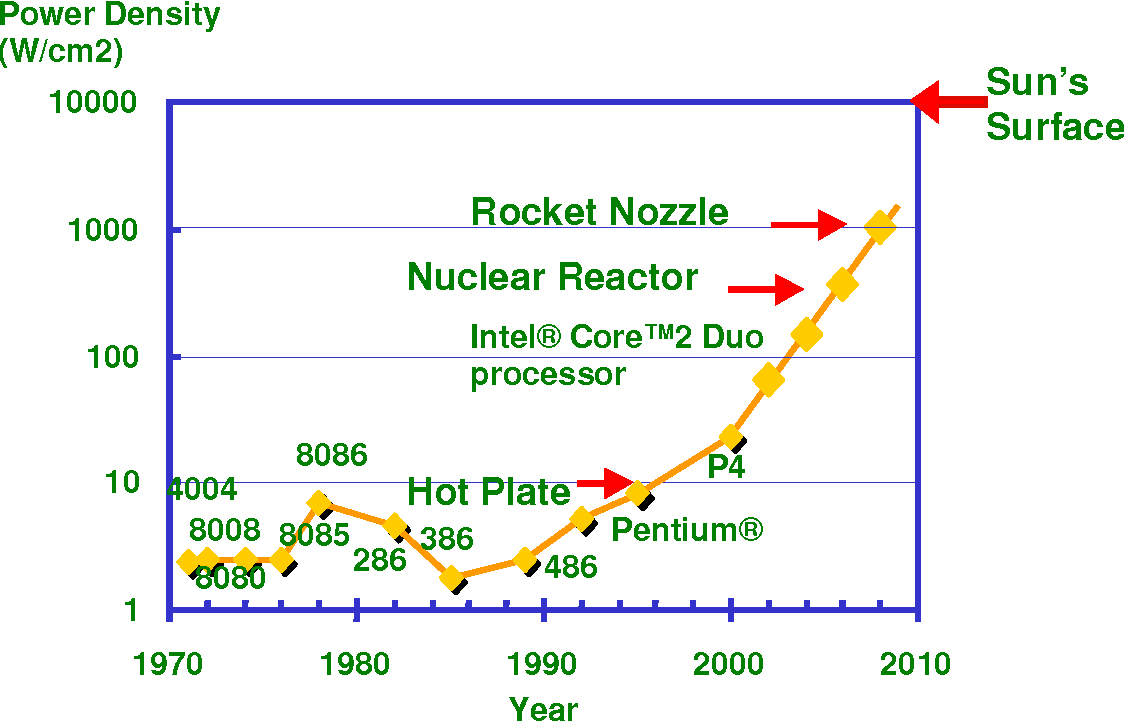
\includegraphics[width=0.72\linewidth]{assets/figures/power-density-1970-2010.png}
\diagramsource{Qian, ``High Performance Network-on-Chips (NoCs) Design'', Figure~1.3, \href{https://www.semanticscholar.org/paper/High-Performance-Network-on-Chips-(NoCs)-Design\%3A-Qian/c83850e832e6792462121d65e58062b9f5d934d5}{Semantic Scholar}; the same chart as \nolinkurl{01-introduction-lecture.pdf}, slide 29 (``Limiting Force: Power Density'')}
\end{minipage}
\end{center}

\paragraph{Conventional wisdom, revisited}
\begin{center}
\begin{tabular}{@{}p{6.6cm}p{6.6cm}@{}}
\toprule
Old conventional wisdom & New conventional wisdom \\
\midrule
Power is free, transistors expensive &
\textbf{``Power wall''}: power expensive, transistors free (can put more on
a chip than can afford to turn on) \\
Increase ILP via compilers, out-of-order, speculation, VLIW &
\textbf{``ILP wall''}: law of diminishing returns on more hardware for ILP \\
Multiplies are slow, memory access is fast &
\textbf{``Memory wall''}: memory slow, multiplies fast ($\sim$200 clock
cycles to DRAM vs.\ 4 clocks for a multiply) \\
Uniprocessor performance $2\times$/1.5~yrs &
Power Wall + ILP Wall + Memory Wall = \textbf{Brick Wall}: uniprocessor
performance now $2\times$/5(?)~yrs \\
\bottomrule
\end{tabular}
\end{center}
\begin{note}
Power Wall + ILP Wall + Memory Wall $\Rightarrow$ a sea change in chip
design: multiple ``cores'' (roughly $2\times$ processors/chip every $\sim$2
years). It is more power-efficient to use many simpler processors than a few
complex ones.
\end{note}

\paragraph{Sea change in chip design -- an illustration}
\begin{itemize}
  \item Intel 4004 (1971): 4-bit, 2312 transistors, 0.4~MHz, 10~$\mu$m PMOS,
  11~mm$^2$.
  \item RISC~II (1983): 32-bit, 5-stage pipeline, 40{,}760 transistors,
  3~MHz, 3~$\mu$m NMOS, 60~mm$^2$.
  \item A 125~mm$^2$, 65~nm CMOS chip could hold roughly
  $2312\times$(RISC~II + FPU + Icache + Dcache) -- \emph{``the processor is
  the new transistor.''}
\end{itemize}

\paragraph{ManyCore chips}
\begin{itemize}
  \item Intel 80-core research chip (Feb 2007): 80 simple cores, two
  FP-engines/core, mesh network, 100M transistors, 65 nm.
  \item Intel Single-Chip Cloud Computer (Aug 2010): 24 ``tiles'' with two
  IA cores/tile, 24-router mesh network (256 GB/s bisection bandwidth), 4
  integrated DDR3 controllers, HW support for message-passing.
  \item Open questions: how to program dozens/hundreds of cores? (e.g.\
  dedicate cores to video/audio, one to the browser, dozens to virus
  scanning?) -- something fundamentally new is needed in the
  software/architecture stack.
\end{itemize}

\subsubsection{The Computer Design Cycle}
\label{sec:computer-design-cycle}

A recurring three-part cycle drives computer design:

\begin{enumerate}
  \item \textbf{Performance}: evaluate existing systems for bottlenecks
  using \emph{benchmarks}.
  \item \textbf{Technology}: simulate new designs and organizations, guided
  by \emph{workloads} and \emph{technology trends}.
  \item \textbf{Cost}: implement the next-generation system, weighing
  \emph{implementation complexity} against cost.
\end{enumerate}

\begin{center}\begin{minipage}{\linewidth}\centering
\begin{tikzpicture}[font=\small]
  \def\r{1.35}
  \draw[very thick,-{Latex[length=3mm]}] (15:\r) arc[start angle=15,end angle=-75,radius=\r];
  \draw[very thick,-{Latex[length=3mm]}] (-105:\r) arc[start angle=-105,end angle=-195,radius=\r];
  \draw[very thick,-{Latex[length=3mm]}] (135:\r) arc[start angle=135,end angle=45,radius=\r];
  \node[align=center,font=\small\bfseries] at (0,0) {Performance,\\Technology\\and Cost};
  \node[anchor=south west,align=left,font=\scriptsize] at (30:1.55)
    {\textbf{1 Performance}\\evaluate existing systems\\for bottlenecks\\\emph{using benchmarks}};
  \node[anchor=north,align=center,font=\scriptsize] at (-90:1.55)
    {\textbf{2 Technology}\\simulate new designs and organizations\\\emph{using workloads}};
  \node[anchor=south east,align=right,font=\scriptsize] at (150:1.55)
    {\textbf{3 Cost}\\implement the next-generation\\system\\\emph{implementation complexity}};
\end{tikzpicture}
\diagramsource{\nolinkurl{01-introduction-lecture.pdf}, slide 36 (``Computer Design Cycle'') (also slides 37, 40)}
\end{minipage}
\end{center}

\subsection{Cost and Price}
\label{sec:cost}

\subsubsection{Price vs.\ cost}
\begin{definition}[Cost and price]
The \textbf{cost} is the total amount spent to produce a product. The
\textbf{price} is the amount for which a finished good is sold.\HP[33]{\S1.6}{27}
\end{definition}
The cost passes through several stages before becoming price; a small
change in cost can have a large impact on price.

\paragraph{Manufacturing cost breakdown.}
\begin{itemize}
  \item \textbf{Component cost}: cost at which components (CPU, DRAM, disk,
  case, \dots) are available to the designer -- typically 40--50\% of list
  price.
  \item \textbf{Direct cost} (recurring): labor, purchasing, scrap,
  warranty -- typically 4--16\% of list price.
  \item \textbf{Gross margin} (non-recurring): R\&D, marketing, sales,
  equipment, rental, maintenance, financing, pre-tax profit, taxes.
  \item \textbf{Average discount}: volume discounts and/or retailer markup,
  typically 15--35\% of list price.
\end{itemize}

\begin{center}\begin{minipage}{\linewidth}\centering
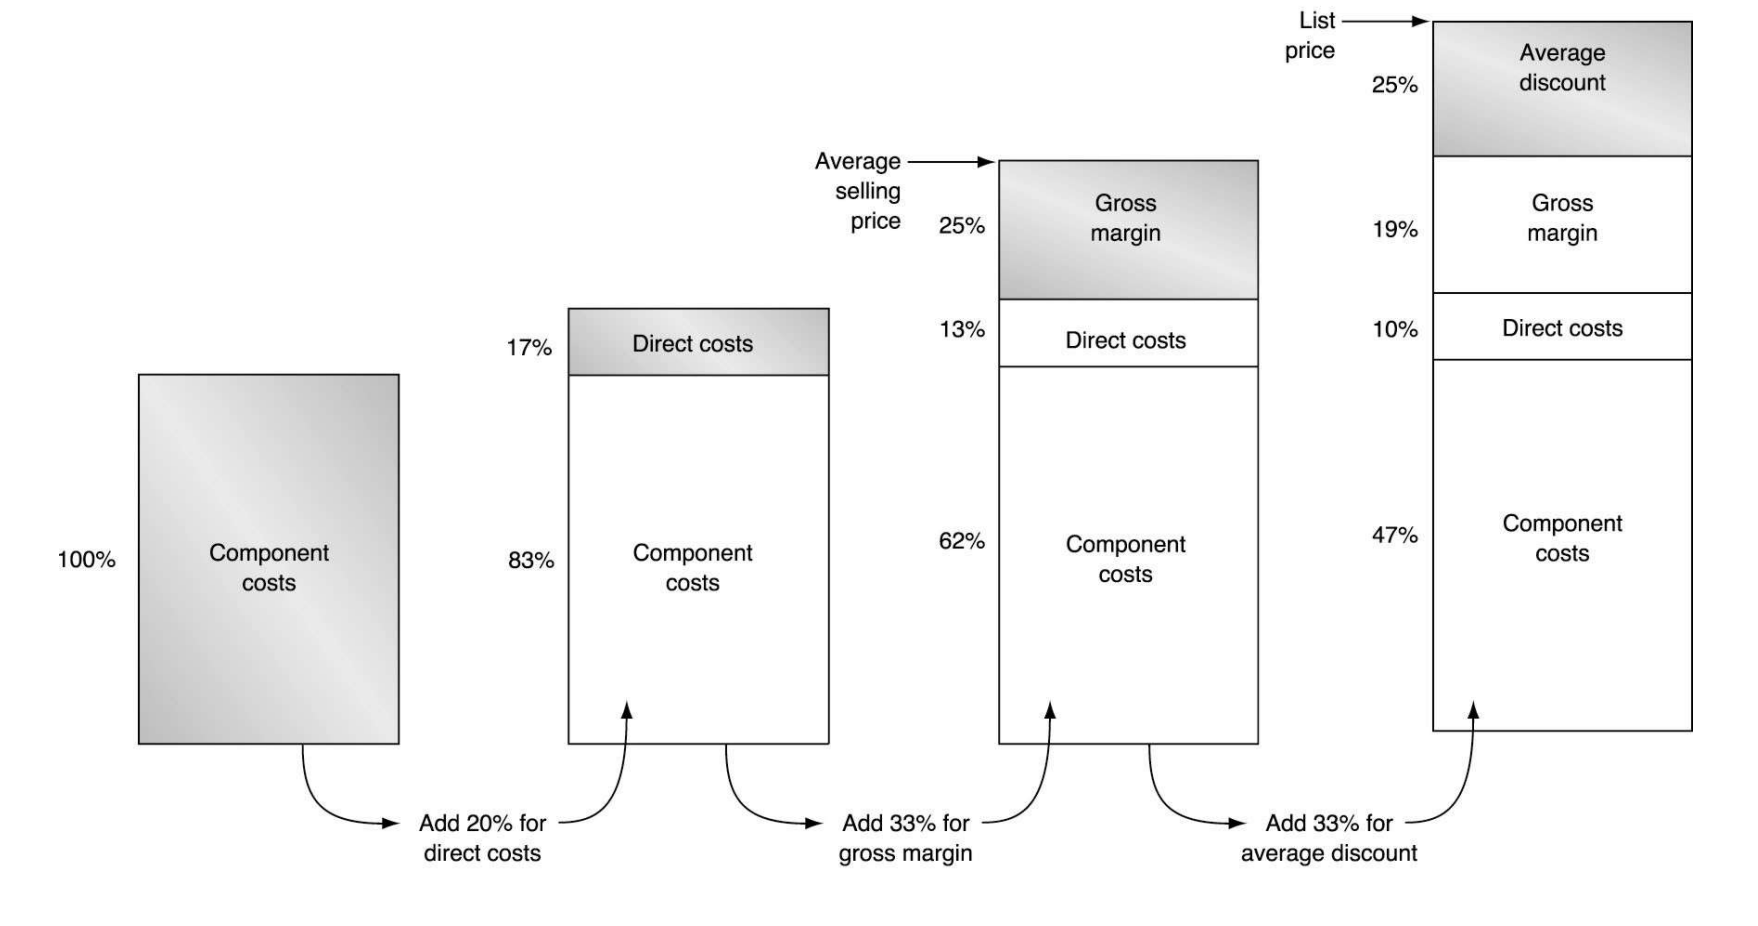
\includegraphics[width=0.95\linewidth]{assets/figures/diag-6.png}
\diagramsource{image supplied by the note-taker (a cost-to-price figure from an earlier edition of H\&P; not in the 5th ed.); the same cost components as \nolinkurl{01-introduction-lecture.pdf}, slide 46 (``Price vs.\ Cost'')}
\end{minipage}
\end{center}
The figure follows one product: adding 20\% for direct costs, 33\% for gross
margin and 33\% for the average discount turns component costs into 47\% of the
list price (direct costs 10\%, gross margin 19\%, discount 25\%). The table gives the
slide's breakdown for three classes of machines.

\begin{center}
\begin{tabular}{@{}lccc@{}}
\toprule
Component (\% of list price) & Mini & W/S & PC \\
\midrule
Component costs & $\sim$20\% & $\sim$27\% & $\sim$55\% \\
Direct costs     & $\sim$8\%  & $\sim$8\%  & $\sim$5\%  \\
Gross margin     & $\sim$47\% & $\sim$32\% & $\sim$20\% \\
Average discount & $\sim$25\% & $\sim$33\% & $\sim$20\% \\
\bottomrule
\end{tabular}
\end{center}
List price includes an average discount of 15--35\% (volume discounts
and/or retailer markup).

\subsubsection{Cost-effective IC design}
\begin{definition}[Yield, volume, feature size]
\textbf{Yield} is the percentage of manufactured components surviving
testing. \textbf{Volume} is the number of units manufactured; higher volume
decreases the list price and improves purchasing efficiency. \textbf{Feature
size} is the minimum size of a transistor or wire in either $x$ or $y$.
\end{definition}
Reduction in feature size from 10~$\mu$m (1971) to 0.045~$\mu$m (2008) has
produced a quadratic rise in transistor count, a linear increase in
performance, and a jump from 4-bit to 64-bit microprocessors.

\subsubsection{Cost of integrated circuits}
Manufacturing stages: wafer growth and testing $\to$ chopping the wafer into
\emph{dies} $\to$ packaging dies into \emph{chips} $\to$ testing a chip. Dies
near the round wafer periphery are wasted (``waist'' area) since only whole
squares fit.

\begin{center}\begin{minipage}{\linewidth}\centering
\begin{tikzpicture}[font=\scriptsize,scale=0.86,every node/.style={scale=0.86}]
  \begin{scope}[shift={(0.00,0)}]
  \fill[black!12] (0,0) circle (1.60);
  \draw[fill=white] (-0.900,-0.900) rectangle ++(0.900,0.900);
  \draw[fill=white] (-0.900,0.000) rectangle ++(0.900,0.900);
  \draw[fill=white] (0.000,-0.900) rectangle ++(0.900,0.900);
  \draw[fill=white] (0.000,0.000) rectangle ++(0.900,0.900);
  \draw[thick] (0,0) circle (1.60);
  \end{scope}
  \begin{scope}[shift={(3.90,0)}]
  \fill[black!12] (0,0) circle (1.60);
  \draw[fill=white] (-1.350,-0.450) rectangle ++(0.900,0.900);
  \draw[fill=white] (-0.450,-1.350) rectangle ++(0.900,0.900);
  \draw[fill=white] (-0.450,-0.450) rectangle ++(0.900,0.900);
  \draw[fill=white] (-0.450,0.450) rectangle ++(0.900,0.900);
  \draw[fill=white] (0.450,-0.450) rectangle ++(0.900,0.900);
  \draw[thick] (0,0) circle (1.60);
  \end{scope}
  \begin{scope}[shift={(7.80,0)}]
  \fill[black!12] (0,0) circle (1.60);
  \draw[fill=white] (-1.350,-0.450) rectangle ++(0.900,0.900);
  \draw[fill=black!45] (-0.450,-1.350) rectangle ++(0.900,0.900);
  \draw[fill=black!45] (-0.450,-0.450) rectangle ++(0.900,0.900);
  \draw[fill=black!45] (-0.450,0.450) rectangle ++(0.900,0.900);
  \draw[fill=black!45] (0.450,-0.450) rectangle ++(0.900,0.900);
  \draw[thick] (0,0) circle (1.60);
  \fill (-0.950,0.750) circle (1.6pt);
  \fill (0.350,1.050) circle (1.6pt);
  \fill (1.050,-0.300) circle (1.6pt);
  \fill (-0.300,-1.100) circle (1.6pt);
  \fill (0.150,0.250) circle (1.6pt);
  \end{scope}
  \begin{scope}[shift={(11.70,0)}]
  \fill[black!12] (0,0) circle (1.60);
  \draw[fill=white] (-1.575,-0.225) rectangle ++(0.450,0.450);
  \draw[fill=white] (-1.125,-1.125) rectangle ++(0.450,0.450);
  \draw[fill=white] (-1.125,-0.675) rectangle ++(0.450,0.450);
  \draw[fill=white] (-1.125,-0.225) rectangle ++(0.450,0.450);
  \draw[fill=white] (-1.125,0.225) rectangle ++(0.450,0.450);
  \draw[fill=black!45] (-1.125,0.675) rectangle ++(0.450,0.450);
  \draw[fill=black!45] (-0.675,-1.125) rectangle ++(0.450,0.450);
  \draw[fill=white] (-0.675,-0.675) rectangle ++(0.450,0.450);
  \draw[fill=white] (-0.675,-0.225) rectangle ++(0.450,0.450);
  \draw[fill=white] (-0.675,0.225) rectangle ++(0.450,0.450);
  \draw[fill=white] (-0.675,0.675) rectangle ++(0.450,0.450);
  \draw[fill=white] (-0.225,-1.575) rectangle ++(0.450,0.450);
  \draw[fill=white] (-0.225,-1.125) rectangle ++(0.450,0.450);
  \draw[fill=white] (-0.225,-0.675) rectangle ++(0.450,0.450);
  \draw[fill=white] (-0.225,-0.225) rectangle ++(0.450,0.450);
  \draw[fill=black!45] (-0.225,0.225) rectangle ++(0.450,0.450);
  \draw[fill=white] (-0.225,0.675) rectangle ++(0.450,0.450);
  \draw[fill=white] (-0.225,1.125) rectangle ++(0.450,0.450);
  \draw[fill=white] (0.225,-1.125) rectangle ++(0.450,0.450);
  \draw[fill=white] (0.225,-0.675) rectangle ++(0.450,0.450);
  \draw[fill=white] (0.225,-0.225) rectangle ++(0.450,0.450);
  \draw[fill=white] (0.225,0.225) rectangle ++(0.450,0.450);
  \draw[fill=black!45] (0.225,0.675) rectangle ++(0.450,0.450);
  \draw[fill=white] (0.675,-1.125) rectangle ++(0.450,0.450);
  \draw[fill=black!45] (0.675,-0.675) rectangle ++(0.450,0.450);
  \draw[fill=white] (0.675,-0.225) rectangle ++(0.450,0.450);
  \draw[fill=white] (0.675,0.225) rectangle ++(0.450,0.450);
  \draw[fill=white] (0.675,0.675) rectangle ++(0.450,0.450);
  \draw[fill=white] (1.125,-0.225) rectangle ++(0.450,0.450);
  \draw[thick] (0,0) circle (1.60);
  \fill (-0.950,0.750) circle (1.6pt);
  \fill (0.350,1.050) circle (1.6pt);
  \fill (1.050,-0.300) circle (1.6pt);
  \fill (-0.300,-1.100) circle (1.6pt);
  \fill (0.150,0.250) circle (1.6pt);
  \end{scope}
  \node[align=center] at (0,-2.15) {large dies,\\grid through the centre:\\4 whole dies};
  \node[align=center] at (3.9,-2.15) {same dies,\\grid shifted:\\5 whole dies};
  \node[align=center] at (7.8,-2.15) {large dies with\\5 defects:\\1 of 5 good};
  \node[align=center] at (11.7,-2.15) {small dies,\\same defects:\\24 of 29 good};
  \draw[fill=black!12] (2.0,-3.35) rectangle ++(0.3,0.3); \node[anchor=west] at (2.35,-3.2) {wafer edge (wasted)};
  \draw[fill=black!45] (5.6,-3.35) rectangle ++(0.3,0.3); \node[anchor=west] at (5.95,-3.2) {die hit by a defect};
  \fill (9.25,-3.2) circle (1.6pt); \node[anchor=west] at (9.4,-3.2) {defect};
\end{tikzpicture}
\diagramsource{\nolinkurl{01-introduction-lecture.pdf}, slide 49 (``Cost of Integrated Circuits''); cf.\ H\&P Fig.~1.15, \hppage{}{30} (wafer photo)}
\end{minipage}
\end{center}

\begin{definition}[Die]
A \emph{die} is the square area of the wafer containing the integrated
circuit. Its cost is determined by the cost of a wafer, the number of dies
that fit on the wafer, and the fraction of dies that work (the
\emph{yield}).
\end{definition}

\begin{prop}[Cost of an integrated circuit]
\begin{align*}
  \text{Cost of IC} &= \frac{\text{die cost} + \text{die testing cost} +
  \text{packaging cost} + \text{final testing cost}}{\text{final test yield}} \\[4pt]
  \text{Die cost} &= \frac{\text{Cost of wafer}}{\text{dies per wafer} \times
  \text{die yield}} \\[4pt]
  \text{Dies per wafer} &= \frac{\pi\,(\text{wafer diameter}/2)^2}{\text{die
  area}} - \frac{\pi\,(\text{wafer diameter})}{\sqrt{2 \times \text{die
  area}}}
\end{align*}\HP[31]{\S1.6}{28}
\end{prop}

\begin{eg}[Dies per wafer]
For a die of 0.7~cm on a side, find the number of dies per wafer of 30~cm
diameter:
\[
  \frac{\pi (30/2)^2}{0.49} - \frac{\pi (30)}{\sqrt{2\times 0.49}} = 1347
  \text{ dies}
\]
\end{eg}

\subsubsection{Calculating die yield}
\begin{prop}[Die yield]
Die yield is the fraction of good dies on a wafer. It depends on defect
density $D$ (defects per unit area) and a process-complexity parameter
$\alpha$ (number of masking levels); a good estimate for CMOS is $\alpha
=4.0$:
\[
  \text{Die Yield} = \text{Wafer Yield} \times \left(1 +
  \frac{(\text{Defects/Unit Area}) \times \text{Die Area}}{\alpha}
  \right)^{-\alpha}
\]\HP{\S1.6}{31}
\end{prop}
\begin{remark}
\textbf{Two yield models.} The slides use $\left(1+\frac{D\cdot A}{\alpha}\right)^{-\alpha}$
with $\alpha\approx4$ (earlier editions of H\&P). The 5th edition uses the
Bose--Einstein model $\text{Die yield}=\text{Wafer yield}\times1/(1+D\times A)^N$,
where $N$ is the process-complexity factor (11.5--15.5 for 40 nm in 2010); with
$D=0.031$ defects/cm$^2$ and $N=13.5$, a 2.25 cm$^2$ die yields 0.40 and a
1 cm$^2$ die 0.66.\HP{\S1.6, Example}{31} Use the formula the exam gives.
\end{remark}

\begin{eg}[Die yield]
The yield of a die 0.7~cm on a side, with defect density 0.6/cm$^2$:
\[
  \left(1 + \frac{0.6 \times 0.49}{4.0}\right)^{-4} = 0.75
\]
\end{eg}

\subsubsection{Real-world example (1993 chip costs)}
\begin{center}
\footnotesize
\begin{tabular}{@{}lrrrrrrrr@{}}
\toprule
Chip & Layers & $\mu$m & Wafer \$ & Def/cm$^2$ &
mm$^2$ & Dies/wf & Yield & Die \$ \\
\midrule
386DX      & 2 & 0.90 & \$900  & 1.0 & 43  & 360 & 71\% & \$4 \\
486DX2     & 3 & 0.80 & \$1200 & 1.0 & 81  & 181 & 54\% & \$12 \\
PowerPC 601& 4 & 0.80 & \$1700 & 1.3 & 121 & 115 & 28\% & \$53 \\
HP PA 7100 & 3 & 0.80 & \$1300 & 1.0 & 196 & 66  & 27\% & \$73 \\
DEC Alpha  & 3 & 0.70 & \$1500 & 1.2 & 234 & 53  & 19\% & \$149 \\
Super SPARC& 3 & 0.70 & \$1700 & 1.6 & 256 & 48  & 13\% & \$272 \\
Pentium    & 3 & 0.80 & \$1500 & 1.5 & 296 & 40  & 9\%  & \$417 \\
\bottomrule
\end{tabular}
\end{center}
\emph{From ``Estimating IC Manufacturing Costs,'' Linley Gwennap,
Microprocessor Report, Aug.\ 2, 1993.}

\subsubsection{Other costs}
\[
  \text{Die Test Cost} = \frac{\text{Test Cost} \times \text{Average Test
  Time}}{\text{Die Yield}}
\]
Packaging cost depends on pin count, heat dissipation, appearance, etc.
Combining die cost with test-and-assembly and packaging gives the total
chip cost -- e.g.\ Pentium (1993): \$417 (die) + \$56 (package + test) =
\$473 total.

\subsubsection{Volume vs.\ cost}
\begin{note}
Rule of thumb (learning-curve effect): ``When volume doubles, costs reduce
10\%.''\; (\emph{A DEC View of Computer Engineering}, C.~G.~Bell,
J.~C.~Mudge, J.~E.~McNamara, 1978.)
\end{note}

\begin{eg}[PC vs.\ workstation volume]
Comparing PC vs.\ workstation shipment volumes (1990--1997), the PC/WS
volume ratio grew from $\sim$59 to $\sim$67 ($2^x = 65 \Rightarrow x
\approx 6.0$), so PC costs fall to roughly $(0.9)^{6.0} = 0.53$ of the
original -- PC costs end up about 47\% lower than workstation costs for the
same functionality.
\end{eg}

\subsubsection{High margins on high-end machines}
R\&D targets a 10\% return on investment: every \$1 of R\&D must generate
\$7--\$13 in sales. High-end machines need more R\&D dollars but sell in
much lower volumes, so they carry much higher margins.

\subsection{Measuring and Comparing Performance}
\label{sec:performance}

\subsubsection{Measuring Performance}
\label{sec:measuring-performance}

\paragraph{Performance metrics}
\begin{definition}[Latency and throughput]
\textbf{Time / latency} is the wall-clock or CPU elapsed time of a task.
\textbf{Throughput} is the number of results produced per second.\HP{\S1.8}{36}
\end{definition}
\begin{remark}
Other measures (MIPS, MFLOPS, clock frequency, cache size) \emph{do not make
sense} on their own as performance measures.
\end{remark}

\begin{center}\begin{minipage}{\linewidth}\centering
\begin{tikzpicture}[font=\small]
  \draw (-0.4,4) -- (5.4,4) -- (3.8,1.8) -- (1.2,1.8) -- cycle;
  \node[align=center] at (2.5,2.95) {Application\\Programming Language\\Compiler};
  \draw[-{Latex}] (5.11,3.6) -- (6,3.6);
  \node[anchor=west,align=left] at (6.05,3.6) {Answers per month\\Operations per second};
  \draw[-{Latex}] (4.09,2.2) -- (6,2.2);
  \node[anchor=west,align=left] at (6.05,2.2) {\textbf{MIPS}: millions of instructions per second\\\textbf{MFLOPS}: millions of FP operations per second};
  \node[draw,thick,minimum width=4.2cm,minimum height=0.55cm] at (2.5,1.25) {Instruction Set Architecture};
  \draw (1.4,0.7) -- (3.6,0.7) -- (5,-2) -- (0,-2) -- cycle;
  \node[align=center,font=\footnotesize] at (2.5,-0.75) {Datapath, Control\\Function Units\\Transistors\\Pins/Wire--I/O};
  \draw[-{Latex}] (3.86,0.2) -- (6,0.2);
  \node[anchor=west] at (6.05,0.2) {Megabytes per second};
  \draw[-{Latex}] (4.59,-1.2) -- (6,-1.2);
  \node[anchor=west] at (6.05,-1.2) {Cycles per second (clock rate)};
\end{tikzpicture}
\diagramsource{\nolinkurl{01-introduction-lecture.pdf}, slide 60 (``Metrics of Performance'')}
\end{minipage}
\end{center}

\paragraph{Measuring tools}
Benchmarks; hardware cost/delay/area/power consumption; simulation (at ISA,
RT, gate, or circuit levels); queuing theory; fundamental laws/principles.

\paragraph{Time}
\begin{definition}[CPU time]
\textbf{CPU time} is the time the CPU is computing, not including time
waiting for I/O or running other programs. \textbf{User CPU time} is the CPU
time spent in the program; \textbf{system CPU time} is the CPU time spent in
the OS performing tasks requested by the program.
\[ \text{CPU time} = \text{User CPU time} + \text{System CPU time} \]
\end{definition}

\begin{eg}[Unix \texttt{time} command]
\texttt{90.7u 12.9s 2:39 65\%} $\Rightarrow$ user CPU 90.7~s, system CPU
12.9~s, elapsed (response) time $2$:$39 = 159$~s; $(90.7+12.9)/159 \times
100 = 65\%$ of elapsed time is CPU time -- the other 35\% is spent in I/O or
running other programs.
\end{eg}

\paragraph{Two notions of ``performance''}
\begin{eg}[Boeing 747 vs.\ Concorde]
\leavevmode
\begin{center}
\begin{tabular}{@{}lccccc@{}}
\toprule
Plane & DC to Paris & Speed & Passengers & Throughput (pmph) \\
\midrule
Boeing 747      & 6.5 hours & 610 mph  & 470 & 286,700 \\
BAD/Sud Concorde & 3 hours  & 1350 mph & 132 & 178,200 \\
\bottomrule
\end{tabular}
\end{center}
\begin{itemize}
  \item \textbf{Time to do the task} (execution time, response time,
  latency): Concorde is $1350/610 = 2.2\times$ faster ($=6.5/3$ hours).
  \item \textbf{Tasks per unit time} (throughput, bandwidth): Boeing is
  $286{,}700/178{,}200 = 1.6\times$ ($60\%$) higher throughput; Concorde is
  only $0.62\times$ the Boeing's throughput.
\end{itemize}
\end{eg}
\begin{remark}
Response time and throughput often trade off against each other.
\end{remark}

\paragraph{Price-performance design: train vs.\ plane}
\begin{eg}[Train vs.\ plane]
\leavevmode
\begin{center}
\small
\begin{tabular}{@{}lccccc@{}}
\toprule
Vehicle & Lab-to-lab & Passengers/trip & Whole job &
Time/person \\
\midrule
Train & 4.0 hours & 2400 & 4.0 hours    & 6.0 sec \\
Plane & 45 min    & 300  & 45$\times$8=6.0 hr & 9.0 sec \\
\bottomrule
\end{tabular}
\end{center}
The plane is over $5\times$ faster individually but needs 50\% more time to
finish the whole job (2400 passengers) -- i.e.\ lower throughput; the
train's per-person time and cost are both lower, so its \emph{cost-performance}
is about 15$\times$ better than the plane's (illustrative example).
\end{eg}

\subsubsection{Comparing Performance and Speedup}
\label{sec:speedup}

\paragraph{Execution-time-based performance}
\begin{definition}[Performance and speedup]
For a given program,
\[
  \text{Performance}_A = \frac{1}{\text{Execution Time}_A}.
\]
``Machine A is $n$ times faster than machine B'' (running the same program)
means
\[
  \text{Speedup} = n = \frac{\text{Performance}_A}{\text{Performance}_B} =
  \frac{\text{Execution Time}_B}{\text{Execution Time}_A}.
\]\HP{\S1.8}{36}
\end{definition}
\begin{eg}
$\text{Exec}_A = 1$~s, $\text{Exec}_B = 10$~s $\Rightarrow$ Speedup $= 10/1 =
10$: machine A is 10 times faster.
\end{eg}

\paragraph{The CPU equation}
\begin{theorem}[The CPU equation]
Let a program execute an \emph{instruction count} $I$ (instructions/program),
with an average of $\CPI$ \emph{cycles per instruction}, on a CPU with
\emph{clock cycle time} $C = 1/\text{clock rate}$ (seconds/cycle). Then
\[
  \text{CPU time} = \frac{\text{Seconds}}{\text{Program}} =
  \frac{\text{Instructions}}{\text{Program}} \times
  \frac{\text{Cycles}}{\text{Instruction}} \times
  \frac{\text{Seconds}}{\text{Cycle}},
\]
\[
  \text{i.e.}\qquad T = I \times \CPI \times C .
\]\HP[51]{\S1.9, The Processor Performance Equation}{48}
\end{theorem}

\begin{eg}[CPU time]
$I = 10{,}000{,}000$ instructions, average $\CPI =2.5$, clock rate
$=200$~MHz ($C = 5\times10^{-9}$~s):
\[
  \text{CPU time} = 10{,}000{,}000 \times 2.5 \times 5\times10^{-9} = 0.125
  \text{ seconds}
\]
\end{eg}

\paragraph{Factors affecting CPU performance}
\begin{center}
\begin{tabular}{@{}lccc@{}}
\toprule
 & Instruction Count $I$ & CPI & Clock Cycle $C$ \\
\midrule
Program                              & X & X &   \\
Compiler                             & X & X &   \\
Instruction Set Architecture (ISA)   & X & X &   \\
Organization (CPU design)            &   & X & X \\
Technology (VLSI)                    &   &   & X \\
\bottomrule
\end{tabular}
\end{center}

\paragraph{Performance-comparison example: changing compiler and CPU}
\begin{eg}[New compiler and faster CPU]
Baseline: $I=10{,}000{,}000$, CPI$=2.5$, clock rate $=200$~MHz. With a new
compiler ($I'=9{,}500{,}000$, CPI$'=3.0$) and a faster CPU (clock rate
$=300$~MHz):
\[
  \text{Speedup} = \frac{I \times CPI \times C}{I' \times CPI' \times C'}
  = \frac{10{,}000{,}000\times2.5\times5\times10^{-9}}
         {9{,}500{,}000\times3.0\times3.33\times10^{-9}}
  = \frac{0.125}{0.095} = 1.32
\]
i.e.\ 32\% faster after the changes.
\end{eg}

\paragraph{Instruction types \& CPI}
\begin{prop}[CPI from instruction classes]
For a program with $n$ instruction classes, $C_i$ = count of instructions of
type $i$, $CPI_i$ = cycles per instruction of type $i$:
\[
  \text{CPU clock cycles} = \sum_{i=1}^{n} \left(CPI_i \times C_i\right)
  \qquad I = \sum_i C_i \qquad CPI = \frac{\text{CPU clock cycles}}{I}
\]\HP{\S1.9}{49}
\end{prop}

\begin{eg}[Two code sequences]
3 instruction classes with $CPI_A=1$, $CPI_B=2$, $CPI_C=3$. Two code
sequences:
\begin{center}
\begin{tabular}{@{}lccc@{}}
\toprule
Sequence & $C_A$ & $C_B$ & $C_C$ \\
\midrule
1 & 2 & 1 & 2 \\
2 & 4 & 1 & 1 \\
\bottomrule
\end{tabular}
\end{center}
Sequence 1: cycles $=2(1)+1(2)+2(3)=10$, $I=5$, $CPI=10/5=2$.
Sequence 2: cycles $=4(1)+1(2)+1(3)=9$, $I=6$, $CPI=9/6=1.5$.
\end{eg}

\paragraph{Instruction frequency \& CPI}
\begin{prop}[CPI from instruction frequencies]
Let $F_i = C_i / I$ be the frequency (fraction) of instruction type $i$.
Then
\[
  CPI = \sum_{i=1}^n \left(CPI_i \times F_i\right)
  \qquad \text{\% of exec.\ time on type } i = \frac{CPI_i \times F_i}{CPI}
\]
\end{prop}

\begin{eg}[RISC typical instruction mix]
\leavevmode
\begin{center}
\begin{tabular}{@{}lccc@{}}
\toprule
Op & $F_i$ & $CPI_i$ & $CPI_i \times F_i$ \\
\midrule
ALU    & 50\% & 1 & 0.50 \\
Load   & 20\% & 5 & 1.00 \\
Store  & 10\% & 3 & 0.30 \\
Branch & 20\% & 2 & 0.40 \\
\midrule
Total  & 100\% & \multicolumn{2}{c}{$CPI = 2.20$} \\
\bottomrule
\end{tabular}
\end{center}
\end{eg}

\paragraph{Performance terminology}
\begin{definition}[``$n\%$ faster'']
``X is $n\%$ faster than Y'' means
\begin{gather*}
  \frac{\text{ExTime}(Y)}{\text{ExTime}(X)} = \frac{\text{Performance}(X)}
  {\text{Performance}(Y)} = 1 + \frac{n}{100},
  \quad\text{i.e.}\\
  n = \frac{100\,(\text{ExTime}(Y) - \text{ExTime}(X))}{\text{ExTime}(X)}.
\end{gather*}
\end{definition}
\begin{eg}
Y takes 15~s, X takes 10~s: $n = 100(15-10)/10 = 50\%$ faster.
\end{eg}

\subsubsection{Amdahl's Law}
\label{sec:amdahl}

\begin{theorem}[Amdahl's Law]
The performance improvement to be gained from using a faster mode of
execution is limited by the fraction of time the faster mode can actually be
used. If an enhancement $E$ accelerates a fraction $F$ (Fraction$_{enhanced}$)
of a task by a factor $S$ (Speedup$_{enhanced}$), and the remainder of the
task is unaffected, then
\[
  \text{ExTime}_{new} = \text{ExTime}_{old} \times \left[(1-F) +
  \frac{F}{S}\right]
  \qquad
  \text{Speedup}_{overall} = \frac{1}{(1-F) + \dfrac{F}{S}}.
\]\HP[48]{\S1.9, Amdahl's Law}{46}
\end{theorem}

\begin{proof}
Normalize $\text{ExTime}_{old}=1=(1-F)+F$. The unaffected part still takes
$1-F$; the affected part now takes $F/S$. So $\text{ExTime}_{new} =
(1-F)+F/S$, and $\text{Speedup} = \text{ExTime}_{old}/\text{ExTime}_{new}$.
\end{proof}

\begin{explanation}
Even an infinitely fast enhancement ($S\to\infty$) gives at most
$\text{Speedup}\to 1/(1-F)$: the part you did not improve becomes the
bottleneck. $F$ must be a fraction of \emph{execution time}, not of
instruction count.
\end{explanation}

\begin{center}\begin{minipage}{\linewidth}\centering
\begin{tikzpicture}[font=\small,x=1.15cm]
  \node[anchor=east] at (-0.15,0.35) {\textbf{Before}};
  \draw (0,0) rectangle (4.95,0.7) node[midway] {Unaffected fraction: $1-F$};
  \draw[fill=black!15] (4.95,0) rectangle (9,0.7) node[midway] {Affected fraction: $F$};
  \node[anchor=east] at (-0.15,-1.55) {\textbf{After}};
  \draw (0,-1.9) rectangle (4.95,-1.2) node[midway] {Unaffected fraction: $1-F$};
  \draw[fill=black!15] (4.95,-1.9) rectangle (6.3,-1.2) node[midway] {$F/S$};
  \draw[dashed,-{Latex}] (0.15,-0.05) -- (0.15,-1.15);
  \draw[dashed,-{Latex}] (4.8,-0.05) -- (4.8,-1.15);
  \node[font=\footnotesize\itshape] at (2.475,-0.6) {unchanged};
  \draw[dashed,-{Latex}] (9,-0.05) -- (6.35,-1.15);
  \node[font=\footnotesize\itshape,anchor=west] at (7.75,-0.75) {sped up by $S$};
  \node[font=\footnotesize] at (4.5,-2.35) {(old time normalized to $1=(1-F)+F$; drawn with $F=0.45$, $S=3$)};
\end{tikzpicture}
\diagramsource{\nolinkurl{01-introduction-lecture.pdf}, slide 83 (``Pictorial Depiction of Amdahl's Law'')}
\end{minipage}
\end{center}

\paragraph{Worked examples}

\begin{eg}[Floating point, single enhancement]
FP instructions improved to run $2\times$ faster; only 10\% of instructions
are FP:
\begin{gather*}
  \text{ExTime}_{new} = \text{ExTime}_{old}\times\left((1-0.1) +
  \frac{0.1}{2}\right) = 0.95\,\text{ExTime}_{old}\\
  \text{Speedup} = \frac{1}{0.95} = 1.053
\end{gather*}
\end{eg}

\begin{eg}[RISC load-CPI enhancement]
Using the RISC instruction mix above, a design enhancement improves the CPI of \texttt{Load} from 5 to 2.
\texttt{Load} instructions are 20\% of the instruction count, but the
fraction of \emph{execution time} they affect is what matters for Amdahl's
Law: from the earlier \% Time table, Load accounts for $F=45\% = 0.45$ of
execution time. $S = 5/2 = 2.5$:
\[
  \text{Speedup}(E) = \frac{1}{(1-0.45) + 0.45/2.5} = \frac{1}{0.55+0.18}
  = 1.37
\]
\emph{Cross-check using the CPU equation directly:} Old $CPI = 2.2$; New
$CPI = 0.5(1) + 0.2(2) + 0.1(3) + 0.2(2) = 1.6$;
Speedup $= \text{old }CPI / \text{new }CPI = 2.2/1.6 = 1.37$ -- matches.
\end{eg}

\begin{eg}[How much must multiplication speed up?]
A program runs in 100~s on a machine where multiply operations take 80~s of
that time. By how much must multiply be sped up to make the whole program:
\begin{itemize}
  \item \textbf{4$\times$ faster?} Need ExTime$_{new}=25$s:
  $25 = (100-80) + 80/n \Rightarrow n = 80/5 = 16$; multiply must be
  16$\times$ faster.
  \item \textbf{5$\times$ faster?} Need ExTime$_{new}=20$s:
  $20 = 20 + 80/n \Rightarrow 0 = 80/n$ -- \textbf{impossible}: no amount of
  multiply speed-up can achieve a 5$\times$ overall speedup, since the
  unaffected 20~s alone is already the target time.
\end{itemize}
\end{eg}

\paragraph{Extending Amdahl's Law to multiple enhancements}
\begin{corollary}[Multiple enhancements]
If enhancements $E_i$ each accelerate a (disjoint) fraction $F_i$ of the
original execution time by factor $S_i$, then
\[
  \text{Speedup} = \frac{1}{\left(1-\sum_i F_i\right) + \sum_i \dfrac{F_i}{S_i}}.
\]
All fractions $F_i$ refer to the \emph{original}, un-enhanced execution time.
\end{corollary}

\begin{eg}[Three enhancements]
$S_1=10, F_1=20\%$; $S_2=15, F_2=15\%$; $S_3=30, F_3=10\%$, each affecting a
disjoint portion of the code, all applied simultaneously:
\begin{align*}
  \text{Speedup} &= \frac{1}{(1-.2-.15-.1) + .2/10 + .15/15 + .1/30}\\
  &= \frac{1}{.55 + .02 + .01 + .0033} = \frac{1}{.5833} = 1.71
\end{align*}
\end{eg}

\paragraph{Corollary: make the common case fast}
\begin{itemize}
  \item All instructions require an instruction fetch; only a fraction
  require a data fetch/store $\Rightarrow$ optimize instruction access over
  data access.
  \item Programs exhibit \emph{locality} (e.g.\ 90\% of time in 10\% of
  code): spatial locality and temporal locality.
  \item Access to small memories is faster $\Rightarrow$ provide a
  \emph{storage hierarchy} so the most frequent accesses go to the
  smallest, closest memories.
\end{itemize}
\begin{center}\begin{minipage}{\linewidth}\centering
\begin{tikzpicture}[font=\small,>=Stealth]
  \node[draw,minimum width=0.6cm,minimum height=0.6cm] (r) at (0,0) {};
  \node[below] at (0,-0.4) {Reg's};
  \node[draw,minimum width=1.2cm,minimum height=1.2cm] (c) at (1.8,0) {};
  \node[below] at (1.8,-0.8) {Cache};
  \node[draw,minimum width=2cm,minimum height=2cm] (m) at (4.3,0) {};
  \node[below] at (4.3,-1.2) {Memory};
  \node[draw,minimum width=3cm,minimum height=2.6cm] (d) at (8,0) {};
  \node[below] at (8,-1.5) {Disk / Tape};
  \draw[<->] (r) -- (c);
  \draw[<->] (c) -- (m);
  \draw[<->] (m) -- (d);
\end{tikzpicture}
\diagramsource{\nolinkurl{01-introduction-lecture.pdf}, slide 91 (``Corollary: Make The Common Case Fast'')}
\end{minipage}
\end{center}

\subsection{Benchmarks and Summarizing Performance}
\label{sec:benchmarking}

\subsubsection{Marketing Metrics: MIPS and MFLOPS}
\label{sec:mips-mflops}

\paragraph{MIPS}
\begin{definition}[MIPS rating]
\[
  \text{MIPS} = \frac{\text{Instruction Count}}{\text{Execution Time}
  \times 10^6} = \frac{\text{Clock Rate}}{CPI \times 10^6}
\]
\end{definition}
MIPS is a rate of operations per unit time; naive reasoning says a bigger
MIPS rating means a faster machine.

\textbf{Wrong!} Three significant problems with using MIPS:
\begin{enumerate}
  \item \textbf{Instruction-set dependent} -- different machines/ISAs are
  not comparable.
  \item \textbf{Varies between programs} on the \emph{same} computer.
  \item \textbf{Can vary inversely with performance!}
\end{enumerate}

\begin{eg}[Higher MIPS, slower program]
Same machine, instruction classes $A$ (CPI 1), $B$ (CPI 2), $C$ (CPI 3),
clock $=100$~MHz. Two compilers:
\begin{center}
\begin{tabular}{@{}lcccc@{}}
\toprule
Compiler & $C_A$ (M) & $C_B$ (M) & $C_C$ (M) \\
\midrule
1 & 5  & 1 & 1 \\
2 & 10 & 1 & 1 \\
\bottomrule
\end{tabular}
\end{center}
\[
  CPI_1 = \frac{5(1)+1(2)+1(3)}{5+1+1} = \frac{10}{7} = 1.43
  \qquad MIPS_1 = \frac{100}{1.43} = 69.9
\]
\[
  CPI_2 = \frac{10(1)+1(2)+1(3)}{10+1+1} = \frac{15}{12} = 1.25
  \qquad MIPS_2 = \frac{100}{1.25} = 80.0
\]
Compiler~2 has the higher MIPS rating -- so is it faster? Compare CPU
\emph{time} instead:
\[
  \text{CPU time}_1 = \frac{7\times10^6\times1.43}{100\times10^6} = 0.10\text{ s}
  \qquad
  \text{CPU time}_2 = \frac{12\times10^6\times1.25}{100\times10^6} = 0.15\text{ s}
\]
\textbf{Compiler~1's program is actually faster, despite its lower MIPS
rating!} -- because it executes fewer instructions overall.
\end{eg}

\begin{note}
MIPS is valid for comparison only when (1) the same program is used, (2) the
same ISA is used, and (3) the same compiler is used -- i.e.\ the compared
programs are identical down to the instruction count.
\end{note}

\paragraph{MFLOPS}
\begin{definition}[MFLOPS rating]
\[
  \text{MFLOPS} = \frac{\text{Number of floating-point operations}}
  {\text{Execution time} \times 10^6}
\]
\end{definition}
A floating-point operation is an add/sub/mul/div on single- or
double-precision values. MFLOPS is generally a better cross-machine
comparison than MIPS (applies even across different ISAs), but it is still
\textbf{program-dependent} (different programs have different fractions of
FP ops; a compiler benchmark, with no FP ops, yields MFLOPS $=0$) and
dependent on the \emph{mix} of FP operation types present. A \emph{Peak
MFLOPS} rating -- obtained from a program of only the simplest FP
instructions -- does not represent real FP programs.

\subsubsection{Benchmarks}
\label{sec:benchmarks}

\paragraph{CPU benchmark suites}
\begin{definition}[Benchmark]
A \emph{benchmark} is a program specifically chosen to measure performance.\HP[41]{\S1.8}{37}
\end{definition}
Five levels of programs, in decreasing order of realism/accuracy:
\begin{enumerate}
  \item Real applications
  \item Modified (scripted) applications
  \item Kernels (extracted hot loops)
  \item Toy benchmarks
  \item Synthetic benchmarks
\end{enumerate}

\paragraph{SPEC (System Performance Evaluation Cooperative)}
\begin{itemize}
  \item \textbf{SPECCPU}: popular desktop CPU-only benchmark suite, split
  into integer and floating-point programs.
  \item \textbf{1989 (1st round)}: 10 programs $\to$ a single SPECmark number.
  \item \textbf{1992 (2nd round)}: SPECint92 (6 integer) and SPECfp92 (14
  FP) programs.
  \item \textbf{1995 (3rd round)}: SPECint95 (8 integer), SPECfp95 (10 FP);
  ``benchmarks useful for 3 years''; a single flag setting for all programs
  (SPECint\_base95, SPECfp\_base95).
  \item \textbf{SPECint2000/SPECfp2000}, and \textbf{SPECCPU2006}.
  \item \textbf{SPECSFS} (NFS file server) and \textbf{SPECWeb} (web
  server) added as server benchmarks.
\end{itemize}

\subsubsection{Summarizing Performance}
\label{sec:summarizing}

\paragraph{Arithmetic mean and weighted arithmetic mean}
\[
  \text{Arithmetic mean} = \frac{1}{n}\sum_{i=1}^n T_i \qquad\text{or
  weighted:}\qquad \sum_i W_i \, T_i
\]
Tracks (weighted) \emph{total} execution time, but gives more weight to
longer-running programs, and different weight choices can make different
machines ``look better.''

\begin{eg}[Which machine is better?]
Two programs P1, P2 on three computers:
\begin{center}
\begin{tabular}{@{}lccc@{}}
\toprule
 & Computer A & Computer B & Computer C \\
\midrule
P1 (sec)   & 1    & 10  & 20 \\
P2 (sec)   & 1000 & 100 & 20 \\
Total time & 1001 & 110 & 40 \\
\bottomrule
\end{tabular}
\end{center}
Which machine is ``better''? With three different weighting schemes for
(P1,P2):
\begin{center}
\begin{tabular}{@{}lccc@{}}
\toprule
Weights (P1/P2) & Computer A & Computer B & Computer C \\
\midrule
.5 / .5     & 500.5 & 55.0  & 20 \\
.909 / .091 & 91.82 & 18.8  & 20 \\
.999 / .001 & 2     & 10.09 & 20 \\
\bottomrule
\end{tabular}
\end{center}
Each weighting scheme picks a different ``winner'' -- illustrating why the
choice of weights is itself contentious.
\end{eg}

\paragraph{Normalized execution time and the geometric mean}
\begin{definition}[Normalized execution time]
Pick a reference machine $R$. The normalized execution time of program $A$
on machine $X$ is (time to run $A$ on $X$) / (time to run $A$ on $R$).
Summarize with the \textbf{geometric mean}
\[
  \sqrt[n]{\prod_{i=1}^{n} \text{Normalized execution time on } i}.
\]\HP[44]{\S1.8, Summarizing Performance Results}{41}
\end{definition}
\begin{remark}
The arithmetic mean of normalized times depends on the choice of reference
machine; the geometric mean is \emph{consistent regardless of the reference
machine}, but it is \emph{not} a good metric for total execution time.
\end{remark}

\paragraph{Summary of means}
\begin{center}
\begin{tabular}{@{}lcp{4.6cm}@{}}
\toprule
Mean & Formula & Property \\
\midrule
Arithmetic & $\dfrac{1}{n}\sum_i T_i$ & Can be weighted; represents total execution time \\
Harmonic   & $\dfrac{n}{\sum_i 1/R_i}$ & Used for rates (e.g.\ throughput) \\
Geometric  & $\left(\prod_i \dfrac{T_i}{T_{r_i}}\right)^{1/n} =
\exp\!\left(\dfrac{1}{n}\sum_i \log\dfrac{T_i}{T_{r_i}}\right)$ &
Consistent, independent of reference machine \\
\bottomrule
\end{tabular}
\end{center}

\paragraph{Performance evaluation, in practice}
Sales are, in part, a function of performance relative to the competition,
and companies invest heavily in improving the product as reported by
performance summaries. Good products result from having \emph{good
benchmarks} and \emph{good ways to summarize performance}. If benchmarks or
summaries are inadequate, vendors must choose between improving the product
for real programs vs.\ improving it to score better on the benchmark --
and, cynically, ``sales almost always wins.'' In the end,
\textbf{execution time remains the real measure of computer performance}.

% =============================================================================
\subsection{Textbook Exercises}
\label{sec:intro-tbx}

\begin{tbexercise}{1.14}{66}{\S1.9 (Amdahl's law), \hppages{}{46}{48}}
Vector mode runs $10\times$ faster than normal mode; the \emph{percentage of
vectorization} is the fraction of time that could use it. (a) Plot net speedup
against percent vectorization. (b) What vectorization gives a speedup of 2? (c) With
a speedup of 2, what percentage of the run time is spent in vector mode? (d) What
vectorization gives half the maximum attainable speedup? (e) Measured vectorization
is 70\%. What vectorization would the compiler team need to equal a further
$2\times$ speedup of the vector unit (beyond the initial $10\times$)?
\end{tbexercise}

\begin{tbexercise}{1.15}{67}{\S1.9, \hppages{}{46}{48}}
An enhancement speeds up a mode of execution by 10. The enhanced mode is used 50\%
of the time, measured as a percentage of the execution time \emph{with} the
enhancement. (a) What speedup was obtained? (b) What percentage of the original
execution time was converted to fast mode?
\end{tbexercise}

\begin{tbexercise}{1.16}{67}{\S1.9, \hppages{}{46}{48}}
(a) A new floating-point unit speeds up FP operations $2\times$; they take 20\% of the
original time. Find the overall speedup. (b) It also slows data-cache accesses
$1.5\times$; they take 10\% of the time. Find the overall speedup now. (c) After the
change, what percentage of the execution time is spent on FP operations and on
data-cache accesses?
\end{tbexercise}

\begin{tbexercise}{1.17}{68}{\S1.9--1.10, \hppages{}{46}{55}}
A dual-core processor runs two applications needing 80\% and 20\% of the resources;
a parallelized portion runs $2\times$ faster. (a) 40\% of the first application is
parallelizable: its speedup alone? (b) 99\% of the second is parallelizable: its
speedup alone? (c), (d) The overall system speedup when each is parallelized.
\end{tbexercise}

\begin{tbexercise}{1.18}{68}{\S1.9, \hppages{}{46}{48}; \S5.1, \hppages{}{348}{350}}
80\% of an application is parallelizable. (a) Speedup with $N$ processors, ignoring
communication. (b) With 8 processors, if each added processor costs 0.5\% of the
original time in communication. (c) With 8 processors, if each doubling of the
processor count adds 0.5\%. (d) The same with $N$ processors. (e) Give the general
equation for the number of processors with the highest speedup when $P\%$ is
parallelizable and each doubling adds 0.5\%.
\end{tbexercise}


\section{Instruction Set Architecture}
\label{sec:isa}
\sources{Lecture ``Review of Instruction Set Architecture''
(\nolinkurl{02-isa-lecture.pdf}); H\&P 5th ed.\ App.~A (Instruction Set
Principles); MIPS reference data card (\texttt{references/}).}

\subsection{The Instruction Set}
\label{sec:instruction-set}

\begin{definition}[Instruction, instruction set]
A computer can only understand binary values; its operation is defined by
predefined binary values called \textbf{instructions}. The
\textbf{instruction set} is the set of all instructions a processor can
perform.\HPA{A}{\S A.1}{2}
\end{definition}

\begin{center}\begin{minipage}{\linewidth}\centering
\begin{tikzpicture}[font=\small,
  layer/.style={draw,minimum width=6.5cm,minimum height=1cm,align=center}]
  \node[layer,fill=white] (sw) at (0,2) {\textbf{Software}};
  \node[layer,fill=black!12] (is) at (0,0.7) {\textbf{Instruction Set}};
  \node[layer,fill=white] (hw) at (0,-0.6) {\textbf{Hardware}};
  \draw[<->,thick] (sw) -- (is);
  \draw[<->,thick] (is) -- (hw);
\end{tikzpicture}
\diagramsource{\nolinkurl{02-isa-lecture.pdf}, slide 5 (``The Instruction Set'')}
\end{minipage}
\end{center}
\begin{note}
The instruction set is the \textbf{interface} between software and hardware.
\end{note}

\subsubsection{Instruction execution cycle}

\begin{center}\begin{minipage}{\linewidth}\centering
\begin{tikzpicture}[font=\small,
  block/.style={draw,fill=black!8,minimum width=2.6cm,minimum height=0.9cm,align=center},
  >=Stealth]
  \node[block] (if) at (0,0)    {Instruction\\Fetch};
  \node[block] (id) at (0,-1.3) {Instruction\\Decode};
  \node[block] (of) at (0,-2.6) {Operand\\Fetch};
  \node[block] (ex) at (0,-3.9) {Execute};
  \node[block] (wb) at (0,-5.2) {Write\\Back};
  \draw[->] (if) -- (id);
  \draw[->] (id) -- (of);
  \draw[->] (of) -- (ex);
  \draw[->] (ex) -- (wb);
  \draw[->] (wb.west) -- ++(-1.0,0) |- (if.west);

  \node[right=0.8cm of if] {Obtain the instruction};
  \node[right=0.8cm of id] {Determine action to be performed};
  \node[right=0.8cm of of] {Obtain the operand data};
  \node[right=0.8cm of ex] {Compute the result (update status)};
  \node[right=0.8cm of wb] {Store the result};
\end{tikzpicture}
\diagramsource{\nolinkurl{02-isa-lecture.pdf}, slide 6 (``Instruction execution cycle'')}
\end{minipage}
\end{center}

\subsection{ISA Styles}
\label{sec:isa-styles}

A generic 2-operand operation:
\begin{center}\begin{minipage}{\linewidth}\centering
\begin{tikzpicture}[font=\small,>=Stealth]
  \node[draw,minimum width=3cm,minimum height=1.2cm] (op) at (0,0) {Operation};
  \draw[->] (-0.9,1.3) -- (-0.9,0.65) node[midway,left]{};
  \draw[->] (0.9,1.3) -- (0.9,0.65);
  \node[above] at (-0.9,1.35) {Input1};
  \node[above] at (0.9,1.35) {Input2};
  \draw[->] (0,-0.65) -- (0,-1.3);
  \node[below] at (0,-1.35) {Output};
\end{tikzpicture}
\diagramsource{\nolinkurl{02-isa-lecture.pdf}, slide 7 (``ISA Styles'')}
\end{minipage}
\end{center}

\begin{definition}[ISA style]
ISA styles differ in \emph{where} the operands of an operation live:
\textbf{Stack}, \textbf{Accumulator}, \textbf{Register-Memory} /
\textbf{Memory-Memory}, and \textbf{Register-Register} (a.k.a.\
\emph{load-store}).\HPA[6]{A}{\S A.2, Figures~A.1--A.2}{3}
\end{definition}

\subsubsection{Stack}

\begin{center}\begin{minipage}{\linewidth}\centering
\begin{tikzpicture}[font=\small]
  \draw (-1.3,0.5) rectangle (1.3,1.0) node[midway] {Stack Element};
  \draw (-1.3,0) rectangle (1.3,0.5) node[midway] {Stack Element};
  \node[draw] (tos) at (-2.6,0.75) {TOS};
  \draw[-{Latex}] (tos) -- (-1.3,0.75);
  \pic at (0,-0.6) {valu};
  \draw[-{Latex}] (-0.65,0) -- (-0.65,-0.6);
  \draw[-{Latex}] (1.3,0.75) -- (1.8,0.75) |- (0.65,-0.3) -- (0.65,-0.6);
  \draw[-{Latex}] (0,-1.6) -- (0,-1.95) -| (2.4,1.35) -| (0.65,1.0);
  \node[anchor=west,font=\footnotesize] at (2.7,0.2) {operands: the top two elements};
  \node[anchor=west,font=\footnotesize] at (2.7,-0.3) {result: pushed back on the stack};
\end{tikzpicture}
\diagramsource{\nolinkurl{02-isa-lecture.pdf}, slide 8 (``ISA Styles: Stack''); cf.\ H\&P Fig.~A.1, \hppage{A}{4}}
\end{minipage}
\end{center}
The operands are on top of the stack; the result is pushed back onto the
stack.
\begin{eg}[$C = A + B$]
\leavevmode
\begin{lstlisting}
PUSH A
PUSH B
ADD
POP C     # C = A + B
\end{lstlisting}
\end{eg}
\begin{remark}
\textbf{(+)} Good code density, simple hardware. \quad
\textbf{(--)} Low parallelism, stack is a bottleneck.
\end{remark}

\subsubsection{Accumulator}

\begin{center}\begin{minipage}{\linewidth}\centering
\begin{tikzpicture}[font=\small]
  \draw (-1.1,0.75) rectangle (1.1,1.25) node[midway] {Accumulator};
  \draw (2.4,-0.6) rectangle (4.2,1.4);
  \foreach \y in {-0.1,0.4,0.9} \draw (2.4,\y) -- (4.2,\y);
  \node[fill=white,inner sep=1pt] at (3.3,0.65) {Memory};
  \pic at (0,0) {valu};
  \draw[-{Latex}] (-0.65,0.75) -- (-0.65,0);
  \draw[-{Latex}] (2.4,0.15) -| (0.65,0);
  \draw[-{Latex}] (0,-1) -- (0,-1.3) -| (-1.7,1) -- (-1.1,1);
\end{tikzpicture}
\diagramsource{\nolinkurl{02-isa-lecture.pdf}, slide 9 (``ISA Styles: Accumulator''); cf.\ H\&P Fig.~A.1, \hppage{A}{4}}
\end{minipage}
\end{center}
One accumulator register is used in all operations.
\begin{eg}[$C = A + B$]
\leavevmode
\begin{lstlisting}
LOAD A    ; put A in Accumulator (AC)
ADD B     ; AC <- AC + B
STORE C   ; C <- AC
\end{lstlisting}
\end{eg}
\begin{remark}
\textbf{(+)} Easy to write a compiler, few instructions. \quad
\textbf{(--)} Very high memory traffic, variable CPI.
\end{remark}

\subsubsection{Memory-Memory}

\begin{center}\begin{minipage}{\linewidth}\centering
\begin{tikzpicture}[font=\small]
  \draw (2.2,-1.6) rectangle (4.0,1.0);
  \foreach \y in {-1.1,-0.6,-0.1,0.4} \draw (2.2,\y) -- (4.0,\y);
  \node[fill=white,inner sep=1pt] at (3.1,-0.35) {Memory};
  \pic at (0,0) {valu};
  \draw[-{Latex}] (2.2,0.7) -| (-0.65,0);
  \draw[-{Latex}] (2.2,0.15) -| (0.65,0);
  \draw[-{Latex}] (0,-1) -- (0,-1.35) -- (2.2,-1.35);
\end{tikzpicture}
\diagramsource{\nolinkurl{02-isa-lecture.pdf}, slide 10 (``ISA Styles: Memory-memory'')}
\end{minipage}
\end{center}
All operands are located in memory.
\begin{eg}[$C = A + B$]
\leavevmode
\begin{lstlisting}
ADD C, A, B    ; C <- A + B   (all three in memory)
\end{lstlisting}
\end{eg}
\begin{remark}
\textbf{(+)} Simple to design and understand. \quad
\textbf{(--)} Accumulator-like bottleneck, heavy memory access.
\end{remark}

\subsubsection{Register-Memory}

\begin{center}\begin{minipage}{\linewidth}\centering
\begin{tikzpicture}[font=\small]
  \draw (-1.1,1.2) rectangle (1.1,1.6) node[midway] {Register};
  \draw (-1.1,0.8) rectangle (1.1,1.2) node[midway] {Register};
  \draw (-1.1,0.4) rectangle (1.1,0.8) node[midway] {Register};
  \pic at (0,0) {valu};
  \draw (2.4,-1.0) rectangle (4.2,1.4);
  \foreach \y in {-0.5,0.0,0.5} \draw (2.4,\y) -- (4.2,\y);
  \node[fill=white,inner sep=1pt] at (3.3,0.25) {Memory};
  \draw[-{Latex}] (-0.65,0.4) -- (-0.65,0);
  \draw[-{Latex}] (2.4,0.2) -| (0.65,0);
  \draw[-{Latex}] (0,-1) -- (0,-1.3) -| (-1.7,1.4) -- (-1.1,1.4);
\end{tikzpicture}
\diagramsource{\nolinkurl{02-isa-lecture.pdf}, slide 11 (``ISA Styles: Register-Memory''); cf.\ H\&P Fig.~A.1, \hppage{A}{4}}
\end{minipage}
\end{center}
Inputs/outputs can be either a register or memory.
\begin{eg}[$C = A + B$]
\leavevmode
\begin{lstlisting}
LOAD  R1, A
ADD   R3, R1, B    ; R3 <- R1 + mem[B]
STORE R3, C
\end{lstlisting}
\end{eg}

\subsubsection{Register-Register (Load-Store)}

\begin{center}\begin{minipage}{\linewidth}\centering
\begin{tikzpicture}[font=\small]
  \draw (-1.1,1.2) rectangle (1.1,1.6) node[midway] {Register};
  \draw (-1.1,0.8) rectangle (1.1,1.2) node[midway] {Register};
  \draw (-1.1,0.4) rectangle (1.1,0.8) node[midway] {Register};
  \pic at (0,0) {valu};
  \draw[-{Latex}] (-0.65,0.4) -- (-0.65,0);
  \draw[-{Latex}] (0.65,0.4) -- (0.65,0);
  \draw[-{Latex}] (0,-1) -- (0,-1.3) -| (-1.7,1.4) -- (-1.1,1.4);
\end{tikzpicture}
\diagramsource{\nolinkurl{02-isa-lecture.pdf}, slide 12 (``ISA Styles: Register-Register''); cf.\ H\&P Fig.~A.1, \hppage{A}{4}}
\end{minipage}
\end{center}
All operations are on registers; dedicated \texttt{Load}/\texttt{Store}
instructions access memory.
\begin{eg}[$C = A + B$]
\leavevmode
\begin{lstlisting}
LOAD  R1, A
LOAD  R2, B
ADD   R3, R1, R2
STORE R3, C
\end{lstlisting}
\end{eg}

\subsubsection{Historical examples}

\begin{center}
\begin{tabular}{@{}llll@{}}
\toprule
Machine & \#GPRs & Architecture style & Year \\
\midrule
Motorola 6800 & 2  & Accumulator                    & 1974 \\
DEC VAX       & 16 & Register-Memory / Memory-Memory & 1977 \\
Intel 8086    & 1  & Extended Accumulator            & 1978 \\
Motorola 68000& 16 & Register-Memory                 & 1980 \\
Intel 80386   & 32 & \textcolor{red}{Register-Memory}& 1985 \\
Power PC      & 32 & \textcolor{blue}{Load-Store}    & 1992 \\
Dec Alpha     & 32 & Load-Store                      & 1992 \\
\bottomrule
\end{tabular}
\end{center}

\subsubsection{Other ISA styles}

\begin{itemize}
  \item \textbf{High-level-language architecture} (e.g.\ Burroughs B5000,
  1960s): instructions map closely to HLL constructs. Fell out of favor due
  to a lack of effective compilers to exploit it.
  \item \textbf{Reduced Instruction Set (RISC) architecture}: simplify the
  hardware, the instruction set, and the instruction format; rely on the
  compiler to synthesize complex operations from simple ones. (Covered in
  detail below.)
\end{itemize}

\subsection{Instruction Set Design}
\label{sec:isa-design}

The design of an instruction set is critical to the operation of a computer
system, and includes many aspects:
\begin{itemize}
  \item Operation repertoire
  \item Addressing modes
  \item Data types
  \item Instruction format
  \item Registers
\end{itemize}

\subsubsection{Simple instruction format}

\begin{center}\begin{minipage}{\linewidth}\centering
\begin{tikzpicture}[font=\small]
  \draw[fill=black!8] (0,0) rectangle ++(1.6,0.8) node[midway]{Opcode};
  \draw[fill=black!8] (1.6,0) rectangle ++(3.4,0.8) node[midway,align=center]{Source Operand\\reference};
  \draw[fill=black!8] (5,0) rectangle ++(3.4,0.8) node[midway,align=center]{Result Operand\\reference};
\end{tikzpicture}
\diagramsource{\nolinkurl{02-isa-lecture.pdf}, slide 16 (``Simple format'')}
\end{minipage}
\end{center}

\begin{definition}[Instruction fields]
\leavevmode
\begin{itemize}
  \item \textbf{Operation Code}: the operation to be performed by the
  processor.
  \item \textbf{Source Operand Reference}: input(s) of the operation --- one
  or more source operands can be involved.
  \item \textbf{Result Operand Reference}: result of the operation.
\end{itemize}
\end{definition}

\subsubsection{Instruction types}

Can be classified into 4 types:\HPA[16]{A}{\S A.5, Figure~A.13}{14}
\begin{itemize}
  \item \textbf{Data processing}: Arithmetic, Logic \quad (e.g.\ \texttt{ADD},
  \texttt{SUB}, \texttt{AND}, \texttt{OR}, \dots)
  \item \textbf{Data storage}: Move data from/to memory \quad (e.g.\
  \texttt{LD}, \texttt{ST})
  \item \textbf{Data movement}: Register and register/IO \quad (e.g.\
  \texttt{MOV})
  \item \textbf{Control}: Test and branch \quad (e.g.\ \texttt{JMP},
  \texttt{CMP})
\end{itemize}

\begin{explanation}
\emph{``There must certainly be instructions for performing the fundamental
arithmetic operations''} --- Burkes, Goldstine and Von Neumann, 1947.
How many programs have an \texttt{IF} statement? $\to$ branch instructions.
How many have a \texttt{Call} statement? $\to$ call/return instructions. How
many programs access memory? \dots and so on: this is how an ISA's operation
repertoire is decided.
\end{explanation}

\subsubsection{Operator types}

\begin{center}
\begin{tabular}{@{}p{3.2cm}p{10.5cm}@{}}
\toprule
Operator type & Example \\
\midrule
Arithmetic \& Logical & Integer arithmetic and logical operations: add, and,
subtract \dots \\
Data transfer & Loads-stores (move instructions on machines with memory
addressing) \\
Control & Branch, jump, procedure call and return, trap \\
System & Operating system call, virtual memory management instructions \\
Floating point & Floating point instructions: add, multiply \\
Decimal & Decimal add, decimal multiply, decimal-to-character conversion \\
String & String move, string compare, string search \\
Graphic & Pixel operations, compression/decompression operations \\
\bottomrule
\end{tabular}
\end{center}

\begin{remark}
Arithmetic, logical, data transfer and control are almost standard
categories for all machines. System instructions are required for
multi-programming environments (support varies). Others can be primitives
(e.g.\ decimal and string on IBM 360 and VAX), provided by a co-processor,
or synthesized by the compiler.
\end{remark}

\subsection{Addressing Modes}
\label{sec:addressing-modes}

\begin{definition}[Addressing mode]
The way the processor refers to the operands is called the
\textbf{addressing mode}.\HPA[11]{A}{\S A.3, Figure~A.6}{9}
\end{definition}
Addressing modes can be classified based on:
\begin{itemize}
  \item \textbf{The source of data}: immediate, registers, memory.
  \item \textbf{The address calculation}: direct, indirect, indexed.
\end{itemize}

\begin{center}
\begin{tabular}{@{}p{4cm}p{7cm}l@{}}
\toprule
Mode & Description & Example \\
\midrule
Immediate & The operand is put in the instruction. & \texttt{ADD R0,\#10} \\
Register & The index of the register containing the operand is specified in
the instruction. & \texttt{ADD R0,R1} \\
Direct & The address of the operand is put in the instruction. & \texttt{ADD
R0,(100)} \\
Register Indirect & The address of the operand is put \emph{in the register}
specified in the instruction. & \texttt{ADD R0,(R1)} \\
Displacement & The address of the operand is Base register $+$
Displacement. & \texttt{LD R1,100(R2)} \\
Indexed & The address of the operand is Base register $+$ Index register. &
\texttt{ADD R3,(R1+R2)} \\
\bottomrule
\end{tabular}
\end{center}

Generic notation (pseudo-RTL) for the same set of modes:

\begin{center}
\begin{tabular}{@{}ll@{}}
\toprule
Mode & Example \\
\midrule
Immediate       & \texttt{add r1 = r2 + 5} \\
Register        & \texttt{add r1 = r2 + r3} \\
Direct          & \texttt{load r1 = M[4000]} \\
Register Indirect & \texttt{add r1 = r2 + M[r2]} \\
Displacement    & \texttt{load r1 = M[r2 + 4000]} \\
Indexed/Base    & \texttt{add r1 = r3 + M[r2 + r3]} \\
Memory Indirect & \texttt{load r1 = M[M[r2]]} \\
PC Relative     & \texttt{branch r1 < r3, 1000} \\
Scaled          & \texttt{load r1 = M[100 + r3 + r4*d]} \\
\bottomrule
\end{tabular}
\end{center}

\subsubsection{Addressing mode usage (SPEC89 on VAX)}

\begin{center}\begin{minipage}{\linewidth}\centering
\begin{tikzpicture}[font=\scriptsize]
  \node[anchor=east] at (-0.85,-0.300) {Memory indirect};
  \node[anchor=east,font=\tiny] at (-0.08,0.000) {TeX};
  \draw[fill=white] (0,-0.120) rectangle (0.10,0.120);
  \node[anchor=west,font=\tiny] at (0.15,0.000) {1\%};
  \node[anchor=east,font=\tiny] at (-0.08,-0.300) {spice};
  \draw[fill=black!35] (0,-0.420) rectangle (0.60,-0.180);
  \node[anchor=west,font=\tiny] at (0.65,-0.300) {6\%};
  \node[anchor=east,font=\tiny] at (-0.08,-0.600) {gcc};
  \draw[fill=black] (0,-0.720) rectangle (0.10,-0.480);
  \node[anchor=west,font=\tiny] at (0.15,-0.600) {1\%};
  \node[anchor=east] at (-0.85,-1.450) {Scaled};
  \node[anchor=east,font=\tiny] at (-0.08,-1.150) {TeX};
  \node[anchor=west,font=\tiny] at (0.05,-1.150) {0\%};
  \node[anchor=east,font=\tiny] at (-0.08,-1.450) {spice};
  \draw[fill=black!35] (0,-1.570) rectangle (1.60,-1.330);
  \node[anchor=west,font=\tiny] at (1.65,-1.450) {16\%};
  \node[anchor=east,font=\tiny] at (-0.08,-1.750) {gcc};
  \draw[fill=black] (0,-1.870) rectangle (0.60,-1.630);
  \node[anchor=west,font=\tiny] at (0.65,-1.750) {6\%};
  \node[anchor=east] at (-0.85,-2.600) {Register deferred};
  \node[anchor=east,font=\tiny] at (-0.08,-2.300) {TeX};
  \draw[fill=white] (0,-2.420) rectangle (2.40,-2.180);
  \node[anchor=west,font=\tiny] at (2.45,-2.300) {24\%};
  \node[anchor=east,font=\tiny] at (-0.08,-2.600) {spice};
  \draw[fill=black!35] (0,-2.720) rectangle (0.30,-2.480);
  \node[anchor=west,font=\tiny] at (0.35,-2.600) {3\%};
  \node[anchor=east,font=\tiny] at (-0.08,-2.900) {gcc};
  \draw[fill=black] (0,-3.020) rectangle (1.10,-2.780);
  \node[anchor=west,font=\tiny] at (1.15,-2.900) {11\%};
  \node[anchor=east] at (-0.85,-3.750) {Immediate};
  \node[anchor=east,font=\tiny] at (-0.08,-3.450) {TeX};
  \draw[fill=white] (0,-3.570) rectangle (4.30,-3.330);
  \node[anchor=west,font=\tiny] at (4.35,-3.450) {43\%};
  \node[anchor=east,font=\tiny] at (-0.08,-3.750) {spice};
  \draw[fill=black!35] (0,-3.870) rectangle (1.70,-3.630);
  \node[anchor=west,font=\tiny] at (1.75,-3.750) {17\%};
  \node[anchor=east,font=\tiny] at (-0.08,-4.050) {gcc};
  \draw[fill=black] (0,-4.170) rectangle (3.90,-3.930);
  \node[anchor=west,font=\tiny] at (3.95,-4.050) {39\%};
  \node[anchor=east] at (-0.85,-4.900) {Displacement};
  \node[anchor=east,font=\tiny] at (-0.08,-4.600) {TeX};
  \draw[fill=white] (0,-4.720) rectangle (3.20,-4.480);
  \node[anchor=west,font=\tiny] at (3.25,-4.600) {32\%};
  \node[anchor=east,font=\tiny] at (-0.08,-4.900) {spice};
  \draw[fill=black!35] (0,-5.020) rectangle (5.50,-4.780);
  \node[anchor=west,font=\tiny] at (5.55,-4.900) {55\%};
  \node[anchor=east,font=\tiny] at (-0.08,-5.200) {gcc};
  \draw[fill=black] (0,-5.320) rectangle (4.00,-5.080);
  \node[anchor=west,font=\tiny] at (4.05,-5.200) {40\%};
  \draw (0,0.25) -- (0,-5.45) -- (6.1,-5.45);
  \draw (0.0,-5.45) -- (0.0,-5.52) node[below,font=\tiny] {0\%};
  \draw (1.0,-5.45) -- (1.0,-5.52) node[below,font=\tiny] {10\%};
  \draw (2.0,-5.45) -- (2.0,-5.52) node[below,font=\tiny] {20\%};
  \draw (3.0,-5.45) -- (3.0,-5.52) node[below,font=\tiny] {30\%};
  \draw (4.0,-5.45) -- (4.0,-5.52) node[below,font=\tiny] {40\%};
  \draw (5.0,-5.45) -- (5.0,-5.52) node[below,font=\tiny] {50\%};
  \draw (6.0,-5.45) -- (6.0,-5.52) node[below,font=\tiny] {60\%};
  \node at (3,-6.05) {Frequency of the addressing mode};
\end{tikzpicture}
\diagramsource{\nolinkurl{02-isa-lecture.pdf}, slide 25 (``Addressing mode use''); values checked against H\&P Fig.~A.7, \hppage{A}{11}}
\end{minipage}
\end{center}
\emph{Focus on immediate and displacement modes since they are used the
most} across TeX, spice, and gcc.\HPA[13]{A}{\S A.3, Figures~A.7--A.10}{11}

\subsubsection{Displacement value size}

Measured as number of bits needed; both integer-average and
floating-point-average workloads show most displacement values fit in a
small number of bits, with the bulk of accesses needing $\le 15$ bits and a
long tail:

\begin{center}\begin{minipage}{\linewidth}\centering
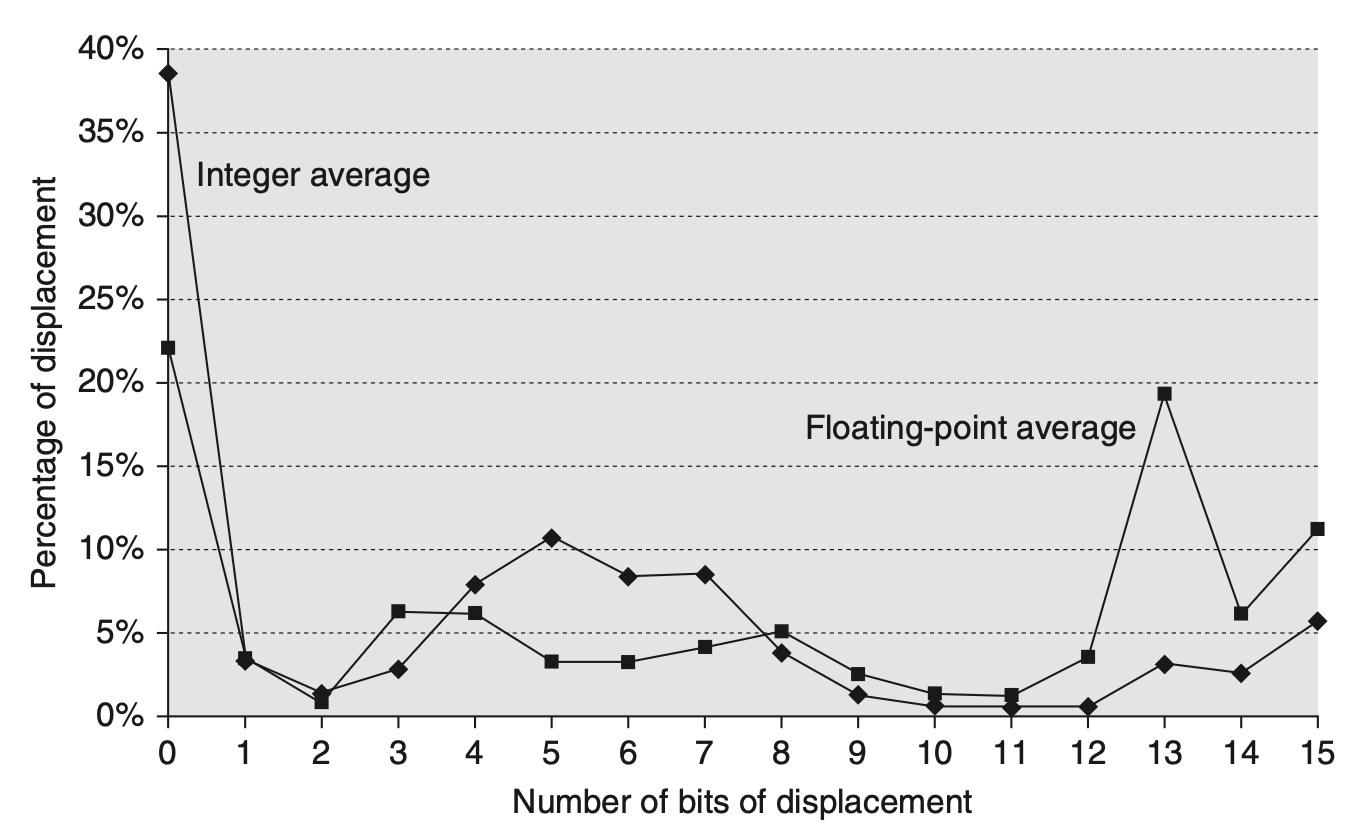
\includegraphics[width=0.8\linewidth]{assets/figures/diag-21.png}
\diagramsource{H\&P Fig.~A.8, \hppage{A}{12} (image supplied by the note-taker); the same chart as \nolinkurl{02-isa-lecture.pdf}, slide 26 (``Addressing mode'')}
\end{minipage}
\end{center}

\subsubsection{Design questions raised by addressing modes}

\begin{itemize}
  \item Is Memory-indirect addressing necessary?
  \item Is Scaled addressing necessary?
  \item Is Register addressing necessary?
  \item How long should a displacement value be?
  \item How long should an immediate value be?
\end{itemize}

\subsection{Operand Types and Sizes}
\label{sec:operands}

\begin{itemize}
  \item \textbf{Character}:
  \begin{itemize}
    \item ASCII (8-bit): almost always used.
    \item Unicode (16-bit): sometimes.
  \end{itemize}
  \item \textbf{Integer}: 2's complement.
  \begin{itemize}
    \item Short: 16 bit.
    \item Long: 32 bit.
  \end{itemize}
  \item \textbf{Floating point}:
  \begin{itemize}
    \item Single precision: 32 bit.
    \item Double precision: 64 bit.
  \end{itemize}
  \item \textbf{Business}: Binary Coded Decimal (BCD) -- accurately
  represents decimal fractions.
  \item \textbf{DSP}: Fixed point, block floating point.
  \item \textbf{Graphic}: RGBA or XYZW, using 8-bit, 16-bit, or single
  precision floating point components.
\end{itemize}

\begin{remark}
Design questions: Should the CPU support all these operand types? Should it
support very big-size operands? Is DSP data used frequently enough to add
dedicated support? Is BCD used in most operations? How about RGBA?
\end{remark}

\subsection{Instruction Format}
\label{sec:instruction-format}

\begin{itemize}
  \item Instructions must be encoded to binary values.\HPA[24]{A}{\S A.7, Figure~A.18}{21}
  \item This affects the size of the compiled program.
  \item Easy to decode $\Rightarrow$ simple to implement.
  \item Should support as many registers and addressing modes as possible.
\end{itemize}

\begin{center}\begin{minipage}{\linewidth}\centering
\begin{tikzpicture}[font=\scriptsize]
  % variable length
  \draw[fill=black!8] (0,1.6) rectangle ++(1.4,0.8) node[midway]{Opcode};
  \draw[fill=black!8] (1.4,1.6) rectangle ++(1.5,0.8) node[midway,align=center]{Addr\\Specifier};
  \draw[fill=black!8] (2.9,1.6) rectangle ++(1.3,0.8) node[midway,align=center]{Addr\\Field};
  \draw[fill=black!8] (4.2,1.6) rectangle ++(0.6,0.8) node[midway]{\dots};
  \draw[fill=black!8] (4.8,1.6) rectangle ++(1.5,0.8) node[midway,align=center]{Addr\\Specifier};
  \draw[fill=black!8] (6.3,1.6) rectangle ++(1.3,0.8) node[midway,align=center]{Addr\\Field};
  \node[right] at (7.8,2.0) {Variable instruction length (e.g.\ VAX, X86)};

  % fixed length
  \draw[fill=black!8] (0,0) rectangle ++(1.4,0.8) node[midway]{Opcode};
  \draw[fill=black!8] (1.4,0) rectangle ++(1.7,0.8) node[midway,align=center]{Addr\\Field 1};
  \draw[fill=black!8] (3.1,0) rectangle ++(1.7,0.8) node[midway,align=center]{Addr\\Field 2};
  \draw[fill=black!8] (4.8,0) rectangle ++(1.7,0.8) node[midway,align=center]{Addr\\Field 3};
  \node[right] at (6.6,0.4) {Fixed instruction length (e.g.\ ARM, MIPS, PowerPC)};
\end{tikzpicture}
\diagramsource{\nolinkurl{02-isa-lecture.pdf}, slide 33 (``Instruction format''); cf.\ H\&P Fig.~A.18, \hppage{A}{22}}
\end{minipage}
\end{center}

\begin{note}
\textbf{Hybrid}: to gain high code density while keeping decode simple, use
2 types of fixed-length instructions (e.g.\ MIPS16, Thumb).
\end{note}

\subsubsection{Register file}

\begin{itemize}
  \item Register is the fastest memory element.
  \item Registers cost much more (per bit) than main memory.
  \item Registers are flexible for the compiler to use.
  \item More registers need more bits to encode in each instruction.
  \item A register file with more locations can be slower to access.
  \item Open design question: how many locations in the register file is
  most effective?
\end{itemize}

\subsection{CISC vs.\ RISC}
\label{sec:cisc-risc}

\subsubsection{Complex Instruction Set Computer (CISC)}

\begin{definition}[CISC]
A \emph{Complex Instruction Set Computer} emphasizes doing more with each
instruction, so programs need fewer instructions (more compact code).
\end{definition}
\begin{itemize}
  \item Emphasizes doing more with each instruction $\Rightarrow$ fewer
  instructions per program (more compact code).
  \item Motivated by the \textbf{high cost of memory} and hard-disk capacity
  when original CISC architectures were proposed:
  \begin{itemize}
    \item M6800: 16K RAM = \$500, 40M hard disk = \$55{,}000.
    \item M68000: 64K RAM = \$200, 10M HD = \$5{,}000.
  \end{itemize}
  \item Original CISC architectures evolved with faster, more complex CPU
  designs, but backward instruction-set compatibility had to be maintained.
  \item Wide variety of addressing modes: 14 in MC68000, 25 in MC68020.
  \item A number of instruction modes for the location and number of
  operands: the VAX has 0- through 3-address instructions.
  \item Variable-length instruction encoding.
\end{itemize}

\begin{eg}[Motorola 680X0]
18 addressing modes (data/address
register direct, immediate, absolute short/long, address register indirect
with post-/pre-increment, displacement, indexed, memory indirect
pre-/post-indexed, PC-relative variants, \dots). GPR ISA (Register-Memory).
Operand size ranges from 1 to 32 bits (1, 2, 4, 8, 10, or 16 bytes).
Instructions are stored in 16-bit words; the smallest instruction is 2 bytes
(one word); the longest is 5 words (10 bytes).
\end{eg}

\begin{eg}[Intel IA-32, x86 (80386)]
12 addressing modes
(register, immediate, direct, base, base+displacement,
index+displacement, scaled-index+displacement, based index, based scaled
index, based index+displacement, based scaled index+displacement,
relative). GPR ISA (Register-Memory). Operand sizes 8, 16, 32, 48, 64, or 80
bits; also supports string operations. The smallest instruction is one
byte; the longest is 12 bytes. The first bytes generally contain the
opcode, mode specifiers, and register fields; the remainder are for address
displacement and immediate data.
\end{eg}

\subsubsection{Reduced Instruction Set Computer (RISC)}

\begin{definition}[RISC]
A \emph{Reduced Instruction Set Computer} focuses on reducing the number and
complexity of instructions, aiming for $\CPI \le 1$.\HPA[39]{A}{\S A.9}{32}
\end{definition}
\begin{itemize}
  \item Focuses on reducing the number and complexity of instructions.
  \item Reduced CPI: goal of at least one instruction per clock cycle
  (\textcolor{blue}{CPI $=1$ or less}).
  \item Designed with pipelining in mind.
  \item Fixed-length instruction encoding.
  \item Only load and store instructions access memory.
  \item \textcolor{blue}{(Thus more instructions are executed than CISC.)}
  \item Simplified addressing modes -- usually limited to immediate,
  register indirect, register displacement, indexed.
  \item Delayed loads and branches.
  \item Instruction pre-fetch and speculative execution.
  \item Examples: MIPS, SPARC, PowerPC, Alpha.
\end{itemize}

\begin{eg}[HP Precision Architecture (HP PA-RISC)]
7 addressing
modes: register, immediate, base with displacement, base with scaled index
and displacement, predecrement, postincrement, PC-relative. Five operand
sizes ranging in powers of two from 1 to 16 bytes. Instruction set has 12
different formats, all 32 bits in length.
\end{eg}

\begin{eg}[Alpha AXP]
4 addressing modes: register direct,
immediate, register indirect with displacement, PC-relative. Four operand
sizes: 1, 2, 4, or 8 bytes. Instruction set has 7 different formats, all 32
bits in length.
\end{eg}

\subsection{Case Study: MIPS}
\label{sec:mips}

\subsubsection{Overview}

\begin{itemize}
  \item Instruction categories: Load/Store, Computational, Jump and Branch,
  Floating Point (coprocessor), Memory Management, Special.
  \item 3 instruction formats: all \textbf{32 bits wide}.
\end{itemize}

\begin{center}\begin{minipage}{\linewidth}\centering
\begin{tikzpicture}[font=\small]
  \node[draw,minimum width=1.6cm,minimum height=2.4cm,align=center] (regs) at (0,0) {R0 -- R31};
  \node[above] at (0,1.35) {Registers};
  \draw[draw,minimum width=1.6cm] (2.4,0.9) rectangle ++(1.6,0.4) node[midway]{PC};
  \draw[draw,minimum width=1.6cm] (2.4,0.4) rectangle ++(1.6,0.4) node[midway]{HI};
  \draw[draw,minimum width=1.6cm] (2.4,-0.1) rectangle ++(1.6,0.4) node[midway]{LO};
\end{tikzpicture}
\diagramsource{\nolinkurl{02-isa-lecture.pdf}, slide 42 (``The MIPS ISA'')}
\end{minipage}
\end{center}

\begin{center}\begin{minipage}{\linewidth}\centering
\begin{tikzpicture}[font=\scriptsize]
  \draw[fill=black!8] (0,1.6) rectangle ++(1.2,0.8) node[midway]{OP};
  \draw[fill=black!8] (1.2,1.6) rectangle ++(1.2,0.8) node[midway]{rs};
  \draw[fill=black!8] (2.4,1.6) rectangle ++(1.2,0.8) node[midway]{rt};
  \draw[fill=black!8] (3.6,1.6) rectangle ++(1.2,0.8) node[midway]{rd};
  \draw[fill=black!8] (4.8,1.6) rectangle ++(1.2,0.8) node[midway]{shamt};
  \draw[fill=black!8] (6.0,1.6) rectangle ++(1.2,0.8) node[midway]{funct};
  \node[right] at (7.4,2.0) {R-format};

  \draw[fill=black!8] (0,0.4) rectangle ++(1.2,0.8) node[midway]{OP};
  \draw[fill=black!8] (1.2,0.4) rectangle ++(1.2,0.8) node[midway]{rs};
  \draw[fill=black!8] (2.4,0.4) rectangle ++(1.2,0.8) node[midway]{rt};
  \draw[fill=black!8] (3.6,0.4) rectangle ++(3.6,0.8) node[midway]{immediate};
  \node[right] at (7.4,0.8) {I-format};

  \draw[fill=black!8] (0,-0.8) rectangle ++(1.2,0.8) node[midway]{OP};
  \draw[fill=black!8] (1.2,-0.8) rectangle ++(6,0.8) node[midway]{jump target};
  \node[right] at (7.4,-0.4) {J-format};
\end{tikzpicture}
\diagramsource{\nolinkurl{02-isa-lecture.pdf}, slide 42 (``The MIPS ISA''); cf.\ H\&P Fig.~A.22, \hppage{A}{35}}
\end{minipage}
\end{center}

\subsubsection{MIPS (RISC) design principles}

\begin{noot}{MIPS (RISC) design principles}
\begin{itemize}
  \item \textbf{Simplicity favors regularity}\HPA[39]{A}{\S A.9 (MIPS)}{32}: fixed-size instructions,
  small number of instruction formats, opcode always in the first 6 bits.
  \item \textbf{Smaller is faster}: limited instruction set, limited number
  of registers in the register file, limited number of addressing modes.
  \item \textbf{Make the common case fast}: arithmetic operands from the
  register file (load-store machine), allow instructions to contain
  immediate operands.
  \item \textbf{Good design demands good compromises}: same instruction
  length, single instruction format $\Rightarrow$ compromise of exactly 3
  instruction formats.
\end{itemize}
\end{noot}

\subsubsection{MIPS instruction-class distribution (SPEC2006)}

\begin{center}
\begin{tabular}{@{}lcc@{}}
\toprule
Instruction Class & Integer & Floating Point \\
\midrule
Arithmetic    & 16\% & 48\% \\
Data transfer & 35\% & 36\% \\
Logical       & 12\% & 4\%  \\
Cond.\ Branch & 34\% & 8\%  \\
Jump          & 2\%  & 0\%  \\
\bottomrule
\end{tabular}
\end{center}

\subsubsection{MIPS register convention}

\begin{center}
\begin{tabular}{@{}llll@{}}
\toprule
Name & Register \# & Usage & Preserve on call? \\
\midrule
\$zero      & 0     & constant 0 (hardware)         & n.a. \\
\$at        & 1     & reserved for assembler        & n.a. \\
\$v0--\$v1  & 2--3  & returned values                & no \\
\$a0--\$a3  & 4--7  & arguments                      & yes \\
\$t0--\$t7  & 8--15 & temporaries                    & no \\
\$s0--\$s7  & 16--23& saved values                   & yes \\
\$t8--\$t9  & 24--25& temporaries                    & no \\
\$k0--\$k1  & 26--27& reserved for operating system  & n.a. \\
\$gp        & 28    & global pointer                 & yes \\
\$sp        & 29    & stack pointer                  & yes \\
\$fp        & 30    & frame pointer                  & yes \\
\$ra        & 31    & return address (hardware)      & yes \\
\bottomrule
\end{tabular}
\end{center}

\subsubsection{MIPS endianness}

\begin{center}\begin{minipage}{\linewidth}\centering
\begin{tikzpicture}[font=\scriptsize]
  \draw (1.00,0) rectangle ++(0.7,0.5) node[midway] {\texttt{0A}};
  \draw (1.70,0) rectangle ++(0.7,0.5) node[midway] {\texttt{0B}};
  \draw (2.40,0) rectangle ++(0.7,0.5) node[midway] {\texttt{0C}};
  \draw (3.10,0) rectangle ++(0.7,0.5) node[midway] {\texttt{0D}};
  \node at (2.4,0.75) {Register};
  \draw (-0.80,-1.050) rectangle (0.00,-0.550) node[midway] {\texttt{0A}};
  \node[anchor=east] at (-0.88,-0.800) {$a$};
  \draw[-{Latex[length=2mm]}] (1.35,0) |- (0.00,-0.800);
  \draw (-0.80,-1.600) rectangle (0.00,-1.100) node[midway] {\texttt{0B}};
  \node[anchor=east] at (-0.88,-1.350) {$a+1$};
  \draw[-{Latex[length=2mm]}] (2.05,0) |- (0.00,-1.350);
  \draw (-0.80,-2.150) rectangle (0.00,-1.650) node[midway] {\texttt{0C}};
  \node[anchor=east] at (-0.88,-1.900) {$a+2$};
  \draw[-{Latex[length=2mm]}] (2.75,0) |- (0.00,-1.900);
  \draw (-0.80,-2.700) rectangle (0.00,-2.200) node[midway] {\texttt{0D}};
  \node[anchor=east] at (-0.88,-2.450) {$a+3$};
  \draw[-{Latex[length=2mm]}] (3.45,0) |- (0.00,-2.450);
  \node at (-0.40,-2.95) {Memory};
  \node[font=\small\bfseries] at (2.4,-3.0) {Big-endian};
  \begin{scope}[xshift=7.2cm]
  \draw (1.00,0) rectangle ++(0.7,0.5) node[midway] {\texttt{0A}};
  \draw (1.70,0) rectangle ++(0.7,0.5) node[midway] {\texttt{0B}};
  \draw (2.40,0) rectangle ++(0.7,0.5) node[midway] {\texttt{0C}};
  \draw (3.10,0) rectangle ++(0.7,0.5) node[midway] {\texttt{0D}};
  \node at (2.4,0.75) {Register};
  \draw (4.60,-1.050) rectangle (5.40,-0.550) node[midway] {\texttt{0D}};
  \node[anchor=west] at (5.48,-0.800) {$a$};
  \draw[-{Latex[length=2mm]}] (3.45,0) |- (4.60,-0.800);
  \draw (4.60,-1.600) rectangle (5.40,-1.100) node[midway] {\texttt{0C}};
  \node[anchor=west] at (5.48,-1.350) {$a+1$};
  \draw[-{Latex[length=2mm]}] (2.75,0) |- (4.60,-1.350);
  \draw (4.60,-2.150) rectangle (5.40,-1.650) node[midway] {\texttt{0B}};
  \node[anchor=west] at (5.48,-1.900) {$a+2$};
  \draw[-{Latex[length=2mm]}] (2.05,0) |- (4.60,-1.900);
  \draw (4.60,-2.700) rectangle (5.40,-2.200) node[midway] {\texttt{0A}};
  \node[anchor=west] at (5.48,-2.450) {$a+3$};
  \draw[-{Latex[length=2mm]}] (1.35,0) |- (4.60,-2.450);
  \node at (5.00,-2.95) {Memory};
  \node[font=\small\bfseries] at (2.4,-3.0) {Little-endian};
  \end{scope}
\end{tikzpicture}
\diagramsource{\nolinkurl{02-isa-lecture.pdf}, slide 46 (``MIPS - Endianness''); cf.\ H\&P \S A.3, \hppage{A}{7}}
\end{minipage}
\end{center}

\begin{definition}[Endianness]
\leavevmode
\begin{itemize}
  \item \textbf{Big-endian}: most-significant byte at the lowest address of
  a word.
  \item \textbf{Little-endian}: least-significant byte at the lowest
  address of a word.
  \item \textbf{MIPS is big-endian} in this course. (H\&P's MIPS64 has a mode bit that
  selects big or little endian;\HPA{A}{\S A.9}{34} x86 is little-endian.)
\end{itemize}\HPA{A}{\S A.3}{7}
\end{definition}

\subsubsection{R-Format instructions}

\begin{center}\begin{minipage}{\linewidth}\centering
\begin{tikzpicture}[font=\scriptsize]
  \draw[fill=black!8] (0,0) rectangle ++(1.2,0.8) node[midway]{Op};
  \draw[fill=black!8] (1.2,0) rectangle ++(1.2,0.8) node[midway]{Rs};
  \draw[fill=black!8] (2.4,0) rectangle ++(1.2,0.8) node[midway]{Rt};
  \draw[fill=black!8] (3.6,0) rectangle ++(1.2,0.8) node[midway]{Rd};
  \draw[fill=black!8] (4.8,0) rectangle ++(1.2,0.8) node[midway]{Shamt};
  \draw[fill=black!8] (6.0,0) rectangle ++(1.2,0.8) node[midway]{Funct};
\end{tikzpicture}
\diagramsource{\nolinkurl{02-isa-lecture.pdf}, slide 47 (``MIPS R-Format instructions'')}
\end{minipage}
\end{center}

\begin{definition}[R-format fields]
\leavevmode
\begin{itemize}
  \item \textbf{Op}: opcode.
  \item \textbf{Rs}: first source register number.
  \item \textbf{Rt}: second source register number.
  \item \textbf{Rd}: destination register number.
  \item \textbf{Shamt}: shift amount (number of bit positions, left/right).
  \item \textbf{Funct}: extended opcode -- the ALU function that encodes the
  datapath operation. Execution: \texttt{Rd <- Rs func Rt}.
\end{itemize}
\end{definition}

For arithmetic and logical instructions the opcode is always
\texttt{SPECIAL} (\texttt{000000}), and \texttt{Funct} indicates the
specific operation.

\begin{eg}[Encoding \texttt{ADD \$t0, \$s1, \$s2}]
\leavevmode
\begin{lstlisting}
ADD $t0, $s1, $s2
\end{lstlisting}
\begin{center}\begin{minipage}{\linewidth}\centering
\begin{tikzpicture}[font=\scriptsize]
  \foreach \x/\w/\lab in {0/1.2/Special,1.2/1.2/{\$s1},2.4/1.2/{\$s2},3.6/1.2/{\$t0},4.8/1.2/0,6.0/1.2/add}
    \draw[fill=black!8] (\x,0.9) rectangle ++(\w,0.7) node[midway]{\lab};
  \foreach \x/\w/\lab in {0/1.2/0,1.2/1.2/17,2.4/1.2/18,3.6/1.2/8,4.8/1.2/0,6.0/1.2/32}
    \draw[fill=white] (\x,0) rectangle ++(\w,0.7) node[midway]{\lab};
\end{tikzpicture}
\diagramsource{\nolinkurl{02-isa-lecture.pdf}, slide 49 (``Arithmetic instruction'')}
\end{minipage}
\end{center}
Binary: \texttt{000000 10001 10010 01000 00000 100000} \quad =\quad
\texttt{0x02324020}.
\end{eg}

\subsubsection{Logical operations}

\texttt{AND, OR, XOR, NOR} (bit-wise).
\begin{lstlisting}
OR $t0, $t1, $t2    # $t0 = $t1 | $t2
\end{lstlisting}
Shift left / shift right: \texttt{Shamt} indicates the number of bits to
shift.
\begin{eg}[Shift left logical]
\leavevmode
\begin{lstlisting}
SLL $t2, $s0, 8
\end{lstlisting}
Encoding: \texttt{000000 00000 10000 01010 01000 000000}.
\end{eg}

\texttt{Shift Right Arithmetic (SRA)} uses the MSB as the shift-in bit
(sign-extending):
\begin{eg}[Shift right arithmetic]
\leavevmode
\begin{lstlisting}
SRA $t2, $s0, 8
\end{lstlisting}
Encoding: \texttt{000000 00000 10000 01010 01000 000011}.
\end{eg}

\begin{remark}
Design questions: why is there no \texttt{SLA} (shift-left-arithmetic)?
Why is there no \texttt{NOT}?
\end{remark}

\subsubsection{Jump register}

Uses \textbf{register indirect addressing}.
\begin{itemize}
  \item \texttt{JR rs}: jump register. \texttt{Rs} = target address;
  \texttt{Rd}, \texttt{Rt} $= 0$; \texttt{shamt} is a hint field (see the MIPS instruction set reference).
  \item \texttt{JALR rs} / \texttt{JALR rd, rs}: jump and link register.
  \texttt{Rs} = target address; \texttt{Rd} = return address; \texttt{Rt}
  $=0$; \texttt{shamt} is a hint field.
\end{itemize}

\subsubsection{I-Format instructions}

\begin{center}\begin{minipage}{\linewidth}\centering
\begin{tikzpicture}[font=\scriptsize]
  \draw[fill=black!8] (0,0) rectangle ++(1.5,0.8) node[midway]{Opcode};
  \draw[fill=black!8] (1.5,0) rectangle ++(1.5,0.8) node[midway]{Rs};
  \draw[fill=black!8] (3.0,0) rectangle ++(1.5,0.8) node[midway]{Rt};
  \draw[fill=black!8] (4.5,0) rectangle ++(3.5,0.8) node[midway]{16-bit immediate value};
\end{tikzpicture}
\diagramsource{\nolinkurl{02-isa-lecture.pdf}, slide 53 (``MIPS I-Format instructions'')}
\end{minipage}
\end{center}

This format is used for:
\begin{itemize}
  \item Operation with immediate addressing.
  \item Operation with displacement addressing.
  \item Operation with PC-relative addressing.
\end{itemize}

\begin{eg}[Immediate arithmetic and logical]
\texttt{Op}: opcode;
\texttt{Rs}: source register; \texttt{Rt}: destination register;
\texttt{Constant}: immediate value ($-32768$ to $32767$).
\begin{lstlisting}
ADDI $t0, $t1, 0x0005
ORI  $t0, $t1, 0xFF00
\end{lstlisting}
Encodings:
\begin{center}
\texttt{001000 01001 01000 0000000000000101}\\
\texttt{001101 01001 01000 1111111100000000}
\end{center}
(Design question: why is there no \texttt{SUBI}?)
\end{eg}

\begin{eg}[Load-Store (displacement)]
\texttt{Rs}: base register number;
16-bit immediate value: offset added to the base address in \texttt{Rs}.
Effective address $EA = Rs + \text{16-bit immediate value}$. For loads,
\texttt{Rt} is the destination register; for stores, \texttt{Rt} is the
value stored to the \texttt{EA} in memory.
\begin{lstlisting}
LW $t0, 16($t1)
SW $t0, 16($t1)
\end{lstlisting}
Encodings:
\begin{center}
\texttt{100011 01001 01000 0000000000010000}\\
\texttt{101011 01001 01000 0000000000010000}
\end{center}
\end{eg}

\begin{eg}[PC-relative (near branches)]
\texttt{Rs}, \texttt{Rt}: source
register numbers; target address $=$ \texttt{PC} $+$ offset $\times 4$ (PC
already incremented by 4 at this time).
\begin{lstlisting}
BEQ $s0, $s1, 256    # if ($s0 == $s1) goto PC + 256*4;
\end{lstlisting}
Encoding: \texttt{000100 10000 10001 0000000100000000}.
\end{eg}

\subsubsection{J-Format instructions}

\begin{center}\begin{minipage}{\linewidth}\centering
\begin{tikzpicture}[font=\scriptsize]
  \draw[fill=black!8] (0,0) rectangle ++(1.5,0.8) node[midway]{Opcode};
  \draw[fill=black!8] (1.5,0) rectangle ++(5.5,0.8) node[midway]{26-bit Offset};
\end{tikzpicture}
\diagramsource{\nolinkurl{02-isa-lecture.pdf}, slide 59 (``MIPS J-format Instructions'')}
\end{minipage}
\end{center}

Used for \texttt{J} and \texttt{JAL} -- \textbf{pseudo-direct addressing}.
Cannot fit a 32-bit value in the instruction, so target address $=
PC_{31\ldots28} \,\Vert\, (\text{26-bit offset} \times 4)$.
\begin{eg}[Jump]
\leavevmode
\begin{lstlisting}
J 0x01000000
\end{lstlisting}
Encoding: \texttt{000010 01000000000000000000000000}.
\end{eg}

\subsubsection{Moving data without a MOV instruction}

\begin{eg}[Move without MOV]
How to move data from \texttt{\$t0} to \texttt{\$t1} using one MIPS
instruction? MIPS has no dedicated \texttt{MOV}, so it is synthesized:
\[
  \texttt{MOV \$t1, \$t0} \;\equiv\; \texttt{add \$t1, \$t0, \$zero}
\]
\end{eg}

\subsubsection{Atomic operations}

\begin{definition}[Load linked / store conditional]
An atomic Read-Modify-Write operation is built from a pair of instructions:
\texttt{LL} (Load Linked Word) and \texttt{SC} (Store Conditional Word).
\begin{lstlisting}
LL $Rt, offset($Rs)
SC $Rt, offset($Rs)
\end{lstlisting}
If the memory word addressed by \texttt{LL} is modified before the matching
\texttt{SC} to the same address, \texttt{SC} \emph{fails} and returns 0 in
\texttt{\$Rt}. Otherwise, \texttt{SC} stores \texttt{\$Rt} to memory and
returns 1 in \texttt{\$Rt}.\HP{\S5.5}{388}
\end{definition}

\begin{eg}[Atomic swap]
\leavevmode
\begin{lstlisting}
try:  ADD $t0, $zero, $s4   # $t0 = $s4
      LL  $t1, 0($s1)       # $t1 = mem($s1)
      SC  $t0, 0($s1)       # mem($s1) = $t0 (if uncontended)
      BEQ $t0, $zero, try   # if mem($s1) changed meanwhile, retry
                             # else mem($s1) = old $t0
      ADD $s4, $zero, $t1   # $s4 = $t1
\end{lstlisting}
\end{eg}

\subsubsection{Constant (immediate) values}

Small constants are used quite frequently ($\approx 50\%$ of operands in
many common programs):
\begin{eg}[Small and large constants]
\leavevmode
\begin{lstlisting}
# $t0 = 0x1234
ADDI $t0, $zero, 0x1234
\end{lstlisting}
For a 32-bit constant that does not fit in the 16-bit immediate field, use
\texttt{LUI} (Load Upper Immediate) followed by \texttt{ORI}:
\begin{lstlisting}
# $t0 = 0x12345678
LUI $t0, 0x1234
ORI $t0, $t0, 0x5678
\end{lstlisting}
\end{eg}

\subsubsection{Procedure call convention}

\begin{definition}[Procedure call convention]
\leavevmode
\begin{enumerate}
  \item Save the return address.
  \item Save necessary registers.
  \item Callee executes the function.
  \item Restore previously saved registers.
  \item Restore the return address.
  \item Jump to the return address.
\end{enumerate}
\end{definition}
\begin{itemize}
  \item \texttt{JAL label}: jump to a label (procedure); the return address
  is stored in \texttt{\$ra} (register 31).
  \item \texttt{JR}: jump to the address stored in a register.
\end{itemize}

\begin{eg}[Array element swap]
\leavevmode
\begin{lstlisting}
swap(int v[], int k)
{
    int temp;
    temp   = v[k];
    v[k]   = v[k+1];
    v[k+1] = temp;
}
\end{lstlisting}
Assume \texttt{swap} is called as a procedure; \texttt{temp} is register
\texttt{\$15}; arguments in \texttt{\$a1}, \texttt{\$a2}; \texttt{\$16} is a
scratch register.

\begin{lstlisting}
swap:
    addi $sp,$sp,-4     ; create space on stack
    sw   $16, 0($sp)    ; callee-saved register put onto stack
    sll  $t2, $a2,2     ; multiply k by 4
    addu $t2, $a1,$t2   ; address of v[k]
    lw   $15, 0($t2)    ; load v[k]
    lw   $16, 4($t2)    ; load v[k+1]
    sw   $16, 0($t2)    ; store v[k+1] into v[k]
    sw   $15, 4($t2)    ; store old value of v[k] into v[k+1]
    lw   $16, 0($sp)    ; callee-saved register restored from stack
    addi $sp,$sp, 4     ; restore top of stack
    jr   $31            ; return to place that called swap
\end{lstlisting}
\end{eg}

\begin{eg}[Recursive factorial]
\leavevmode
\begin{lstlisting}
fact:
    addi $sp, $sp, -8   # adjust stack for 2 items
    sw   $ra, 4($sp)    # save return address
    sw   $a0, 0($sp)    # save argument

    slti $t0, $a0, 1    # test for n < 1
    beq  $t0, $zero, L1

    addi $v0, $zero, 1  # if so, result is 1
    addi $sp, $sp, 8     #   pop 2 items from stack
    jr   $ra             #   and return

L1: addi $a0, $a0, -1   # else decrement n
    jal  fact             # recursive call

    lw   $a0, 0($sp)    # restore original n
    lw   $ra, 4($sp)    #   and return address
    addi $sp, $sp, 8    # pop 2 items from stack

    mul  $v0, $a0, $v0  # multiply to get result n*fact(n-1)
    jr   $ra             # and return
\end{lstlisting}
\end{eg}

\subsubsection{Reference tables}

\begin{center}
\begin{tabular}{@{}p{2.6cm}p{2.6cm}p{3.3cm}p{4.6cm}@{}}
\toprule
Instruction & Example & Meaning & Comment \\
\midrule
add            & \texttt{add \$1,\$2,\$3}   & \$1 = \$2 + \$3 & 3 operands; exception possible \\
subtract       & \texttt{sub \$1,\$2,\$3}   & \$1 = \$2 -- \$3 & 3 operands; exception possible \\
add immediate  & \texttt{addi \$1,\$2,100}  & \$1 = \$2 + 100 & + constant; exception possible \\
add unsigned   & \texttt{addu \$1,\$2,\$3}  & \$1 = \$2 + \$3 & 3 operands; no exceptions \\
subtract unsigned & \texttt{subu \$1,\$2,\$3} & \$1 = \$2 -- \$3 & 3 operands; no exceptions \\
add imm.\ unsign. & \texttt{addiu \$1,\$2,100} & \$1 = \$2 + 100 & + constant; no exceptions \\
multiply       & \texttt{mult \$2,\$3}      & Hi,Lo = \$2 $\times$ \$3 & 64-bit signed product \\
multiply unsigned & \texttt{multu \$2,\$3}  & Hi,Lo = \$2 $\times$ \$3 & 64-bit unsigned product \\
divide         & \texttt{div \$2,\$3}       & Lo=\$2$\div$\$3, Hi=\$2 mod \$3 & Lo=quotient, Hi=remainder \\
divide unsigned & \texttt{divu \$2,\$3}     & Lo=\$2$\div$\$3, Hi=\$2 mod \$3 & unsigned quotient \& remainder \\
move from Hi   & \texttt{mfhi \$1}          & \$1 = Hi & used to get copy of Hi \\
move from Lo   & \texttt{mflo \$1}          & \$1 = Lo & used to get copy of Lo \\
\bottomrule
\end{tabular}
\end{center}

\begin{center}
\begin{tabular}{@{}p{2.9cm}p{2.5cm}p{3cm}p{4.3cm}@{}}
\toprule
Instruction & Example & Meaning & Comment \\
\midrule
and            & \texttt{and \$1,\$2,\$3}  & \$1=\$2\&\$3       & 3 reg.\ operands; logical AND \\
or             & \texttt{or \$1,\$2,\$3}   & \$1=\$2\textbar\$3 & 3 reg.\ operands; logical OR \\
xor            & \texttt{xor \$1,\$2,\$3}  & \$1=\$2$\oplus$\$3 & 3 reg.\ operands; logical XOR \\
nor            & \texttt{nor \$1,\$2,\$3}  & \$1=$\sim$(\$2\textbar\$3) & 3 reg.\ operands; logical NOR \\
and immediate  & \texttt{andi \$1,\$2,10}  & \$1=\$2\&10        & logical AND reg, constant \\
or immediate   & \texttt{ori \$1,\$2,10}   & \$1=\$2\textbar10  & logical OR reg, constant \\
xor immediate  & \texttt{xori \$1,\$2,10}  & \$1=$\sim$\$2\&$\sim$10 & logical XOR reg, constant \\
shift left logical & \texttt{sll \$1,\$2,10} & \$1=\$2\textless\textless10 & shift left by constant \\
shift right logical & \texttt{srl \$1,\$2,10} & \$1=\$2\textgreater\textgreater10 & shift right by constant \\
shift right arithm. & \texttt{sra \$1,\$2,10} & \$1=\$2\textgreater\textgreater10 & shift right (sign extend) \\
shift left logical (var) & \texttt{sllv \$1,\$2,\$3} & \$1=\$2\textless\textless\$3 & shift left by variable \\
shift right logical (var) & \texttt{srlv \$1,\$2,\$3} & \$1=\$2\textgreater\textgreater\$3 & shift right by variable \\
shift right arithm.\ (var) & \texttt{srav \$1,\$2,\$3} & \$1=\$2\textgreater\textgreater\$3 & shift right arith.\ by variable \\
\bottomrule
\end{tabular}
\end{center}

\begin{center}
\begin{tabular}{@{}ll@{}}
\toprule
Instruction & Comment \\
\midrule
\texttt{SW 500(R4), R3} & Store word \\
\texttt{SH 502(R2), R3} & Store half \\
\texttt{SB 41(R3), R2}  & Store byte \\
\texttt{LW R1, 30(R2)}  & Load word \\
\texttt{LH R1, 40(R3)}  & Load halfword \\
\texttt{LHU R1, 40(R3)} & Load halfword unsigned \\
\texttt{LB R1, 40(R3)}  & Load byte \\
\texttt{LBU R1, 40(R3)} & Load byte unsigned \\
\texttt{LUI R1, 40}     & Load upper immediate (16 bits shifted left by 16) \\
\bottomrule
\end{tabular}
\end{center}

\begin{center}
\begin{tabular}{@{}lll@{}}
\toprule
& & \\
\midrule
Compare and Branch & \texttt{BEQ rs,rt,offset} & if R[rs]==R[rt] then PC-relative branch \\
                    & \texttt{BNE rs,rt,offset} & \dots not-equal ($\neq$) \\
                    & \texttt{BLEZ rs,offset}   & if R[rs] $\le$ 0 then PC-relative branch \\
                    & \texttt{BGTZ rs,offset}   & \dots greater-than ($>$) \\
                    & \texttt{BLTZ rs,offset}   & \dots less-than ($<$) \\
                    & \texttt{BGEZ rs,offset}   & \dots greater-or-equal ($\ge$) \\
\bottomrule
\end{tabular}
\end{center}

\begin{center}
\begin{tabular}{@{}p{2.7cm}p{3cm}p{7.2cm}@{}}
\toprule
Instruction & Example & Meaning \\
\midrule
branch on equal & \texttt{beq \$1,\$2,100} & if (\$1==\$2) go to PC+4+100; equal test; PC-relative branch \\
branch on not eq.\ & \texttt{bne \$1,\$2,100} & if (\$1!=\$2) go to PC+4+100; not-equal test; PC-relative \\
set on less than & \texttt{slt \$1,\$2,\$3} & if (\$2<\$3) \$1=1; else \$1=0; compare less than; 2's comp. \\
set less than imm. & \texttt{slti \$1,\$2,100} & if (\$2<100) \$1=1; else \$1=0; compare~<~constant; 2's comp. \\
set less than uns. & \texttt{sltu \$1,\$2,\$3} & if (\$2<\$3) \$1=1; else \$1=0; compare less than; natural no.\ \\
set l.t.\ imm.\ uns. & \texttt{sltiu \$1,\$2,100} & if (\$2<100) \$1=1; else \$1=0; compare~<~constant; natural \\
jump            & \texttt{j 10000}   & go to 10000; jump to target address \\
jump register   & \texttt{jr \$31}   & go to \$31; for switch, procedure return \\
jump and link   & \texttt{jal 10000} & \$31 = PC+4; go to 10000; for procedure call \\
\bottomrule
\end{tabular}
\end{center}

\subsubsection{Assembler directives and example programs}

\begin{definition}[Assembler directives]
Common assembler (GAS/SPIM-style) directives: \texttt{.text} (code
section), \texttt{.data} (data section), \texttt{.globl} (export a label),
\texttt{.word} (a 32-bit word constant), \texttt{.space} (reserve $n$
bytes).
\end{definition}

\begin{eg}[Adding two constants]
\leavevmode
\begin{lstlisting}
.text
.globl main
main:
    li   $t0, 0x2         # $t0 <- 0x2
    li   $t1, 0x3         # $t1 <- 0x3
    addu $t2, $t0, $t1    # $t2 <- ADD($t0, $t1)
\end{lstlisting}
which is equivalent to (\texttt{li} pseudo-instruction expanded):
\begin{lstlisting}
.text
.globl main
main:
    ori  $t0, $0, 0x2     # $t0 <- OR(0, 0x2)
    ori  $t1, $0, 0x3     # $t1 <- OR(0, 0x3)
    addu $t2, $t0, $t1    # $t2 <- ADD($t0, $t1)
\end{lstlisting}
\end{eg}

\begin{eg}[Using labeled data]
\leavevmode
\begin{lstlisting}
.data
n:  .word 0x2
m:  .word 0x3
r:  .space 4

.text
.globl main
main:
    lw   $t0, n            # load n to $t0
    lw   $t1, m            # load m to $t1
    addu $t2, $t0, $t1     # $t2 <- ADD($t0, $t1)
    sw   $t2, r            # store $t2 to r
\end{lstlisting}
\end{eg}

\begin{eg}[Indexing into an array (\texttt{la} + displacement)]
\leavevmode
\begin{lstlisting}
.data
n:  .word 0x2, 0x3, 0x4

.text
.globl main
main:
    la   $t5, n             # load address of n to $t5
    lw   $t0, 0($t5)        # load n[0] to $t0
    lw   $t1, 4($t5)        # load n[1] to $t1
    addu $t2, $t0, $t1      # $t2 <- ADD($t0, $t1)
    sw   $t2, 8($t5)        # store $t2 to n[2]
\end{lstlisting}
\end{eg}

\subsubsection{Using the SPIM simulator}

A typical SPIM (QtSpim) workflow to assemble, run, and debug MIPS code:
\begin{enumerate}
  \item \textbf{Start SPIM}: the window shows the integer/FP register file,
  the program's text segment (disassembly), and a message log.
  \item \textbf{Load a program}: \emph{File $\to$ Reinitialize and Load
  File}, then select your assembly (\texttt{.s}) file.
  \item \textbf{Execute}: step or run; the current instruction is
  highlighted, and register changes from the previous instruction are shown.
  \item \textbf{Inspect data}: the \emph{Data} tab shows the user data
  segment and stack contents in memory.
  \item \textbf{Set a breakpoint}: right-click an instruction in the text
  segment and choose \emph{Set Breakpoint} (e.g.\ at a conditional branch).
  \item \textbf{Single-step}: use the step button (F10) to execute the
  program line by line and watch register/memory state evolve.
\end{enumerate}

\subsubsection{Reference}
\emph{MIPS instruction set reference}, course handout
(\texttt{references/mips-reference-data.pdf}); see also the reformatted
version, \texttt{references/mips-reference-readable.pdf}.

% =============================================================================
\subsection{Textbook Exercises}
\label{sec:isa-tbx}

\begin{tbexercise}[A]{A.7}{48}{\S A.2 and \S A.9, \hppages{A}{3}{6}, \hppages{A}{32}{39}}
For \texttt{for (i = 0; i <= 100; i++) \{ A[i] = B[i] + C; \}}, with \texttt{A},
\texttt{B} arrays of 64-bit integers and \texttt{C}, \texttt{i} 64-bit integers, all
kept in memory (at 1000, 3000, 5000, 7000) except while operated on, and registers
lost between iterations: (a) write the MIPS code; how many instructions are executed,
how many data memory references, what is the code size? (b) The same for x86.
\end{tbexercise}

\begin{tbexercise}[A]{A.8}{48}{\S A.2 and \S A.7, \hppages{A}{21}{24}}
Instructions are 12 bits long with 5-bit register (address) fields (32 registers).
(a) Can you encode 3 two-address, 30 one-address and 45 zero-address instructions?
(b) 3 two-address, 31 one-address and 35 zero-address? Explain. (c) With 3 two-address
and 24 zero-address instructions, what is the maximum number of one-address
instructions?
\end{tbexercise}

\begin{tbexercise}[A]{A.9}{49}{\S A.2, Figure~A.2, \hppages{A}{3}{6}}
$A$--$F$ are in memory; opcodes are 8 bits, memory addresses 64 bits, register
addresses 6 bits. (a) For each ISA style (stack, accumulator, register-memory,
load-store), how many addresses appear in each instruction of $C=A+B$, and what is the
code size? (b) For each style write $C=A+B$; $D=A-E$; $F=C+D$, marking destroyed
operands and overhead instructions; give the code size, bytes moved to and from
memory, and the overhead instructions and bytes.
\end{tbexercise}

\begin{tbexercise}[A]{A.10}{49}{\S A.2, \S A.7, \S A.9}
MIPS has 32 general-purpose and 32 floating-point registers. If registers are good,
are more registers better? List and discuss the trade-offs of increasing their number.
\end{tbexercise}

\begin{tbexercise}[A]{A.11}{50}{\S A.3 (alignment), \hppages{A}{7}{8}}
\texttt{struct foo \{ char a; bool b; int c; double d; short e; float f; double g;
char *cptr; float *fptr; int x; \};} What is its size on a 32-bit machine? What is
the minimum size if the members may be reordered? And on a 64-bit machine?
\end{tbexercise}

\begin{tbexercise}[A]{A.22}{54}{\S A.3 (byte order, alignment), \hppages{A}{7}{8}}
The value \texttt{434F 4D50 5554 4552} (hex) is stored in an aligned 64-bit
doubleword. (a) Write the bytes in big-endian order and the ASCII character of each.
(b) The same in little-endian order. (c) Give all misaligned 2-byte words readable in
big-endian order. (d) Give all misaligned 4-byte words readable in little-endian order.
\end{tbexercise}


\section{Pipelining}
\label{sec:pipelining}
\sources{Lecture ``Pipelining'' (\nolinkurl{03-pipelining-lecture.pdf}); H\&P 5th
ed.\ App.~C (Pipelining: Basic and Intermediate Concepts).}

\subsection{What Is Pipelining?}
\label{sec:pipelining-idea}

\begin{definition}[Pipelining]
\textbf{Pipelining} is an implementation technique in which multiple
instructions are overlapped in execution.\HPA{C}{\S C.1}{2}
\end{definition}

Real-life pipelining examples:
\begin{itemize}
  \item Doing laundry (washing, drying, folding multiple loads)
  \item Factory production lines
  \item Traffic (?)
\end{itemize}

\subsubsection{Instruction Pipelining}

\begin{definition}[Instruction pipeline, stage, machine cycle]
\leavevmode
\begin{itemize}
  \item Instruction pipelining is a CPU implementation technique where
  \textbf{multiple operations} on a number of instructions are \textbf{overlapped}.
  \item An instruction execution pipeline involves a number of steps, where each
  step completes a part of an instruction. Each step is called a \emph{pipeline
  stage} or \emph{pipeline segment}.
  \item The stages are connected in a \textbf{linear fashion}: one stage to the
  next, forming the pipeline -- instructions enter at one end, progress through
  the stages, and exit at the other end.
  \item The time to move an instruction one step down the pipeline is equal to
  \emph{the machine cycle} and is determined by the stage with the longest
  processing delay.
\end{itemize}\HPA[10]{C}{\S C.1, The Classic Five-Stage Pipeline}{6}
\end{definition}

\begin{itemize}
  \item Pipelining \textbf{increases} the CPU \textbf{instruction throughput}:
  the number of instructions completed per cycle.
  \begin{itemize}
    \item Under ideal conditions (no stall cycles), instruction throughput is
    one instruction per machine cycle, i.e.\ \textcolor{red}{ideal CPI = 1}.
  \end{itemize}
  \item Pipelining \textbf{does not reduce} the execution time of an
  individual instruction: the time needed to complete all processing steps of
  an instruction (also called \emph{instruction completion latency}).
  \begin{itemize}
    \item Minimum instruction latency $= n$ cycles, where $n$ is the number of
    pipeline stages.
  \end{itemize}
\end{itemize}

\begin{explanation}
\textbf{Why is the ideal CPI equal to 1?} CPI counts how many cycles pass, on
average, between \emph{completions} of instructions -- not how long each
instruction takes. In a $k$-stage pipeline each instruction still needs $k$
cycles from fetch to write-back, but once the pipeline is full a new
instruction enters and an old one leaves every cycle. For $n$ instructions the
pipeline needs $k + (n-1)$ cycles, so
\[
  \CPI = \frac{k + n - 1}{n} \;\longrightarrow\; 1 \quad (n\to\infty).
\]
The fill cost of $k-1$ cycles is paid only once. Stalls caused by hazards add
cycles without completing instructions, which is why real pipelines have
$\CPI = 1 + \text{stall cycles per instruction}$.
\end{explanation}

\subsection{Pipelining Example: Laundry}
\label{sec:laundry}

\begin{eg}[Doing laundry]
Ann, Brian, Cathy, and Dave (A, B, C, D) each have one load of clothes to
wash, dry, and fold.
\begin{itemize}
  \item Washer takes 30 minutes
  \item Dryer takes 40 minutes
  \item ``Folder'' takes 20 minutes
\end{itemize}
\end{eg}

\subsubsection{Sequential laundry}

\begin{center}\begin{minipage}{\linewidth}\centering
\begin{tikzpicture}[x=0.95cm,y=-0.9cm,font=\scriptsize]
  \draw[-{Stealth}] (0,-0.6) -- (12.4,-0.6) node[right] {time (hours)};
  \foreach \t/\lab in {0/6PM,1.5/7,3.5/8,5.5/9,7.5/10,9.5/11,11.5/Midnight}
    \node at (\t,-1.0) {\lab};
  \foreach \task/\row in {A/0,B/1,C/2,D/3}{
    \pgfmathsetmacro{\xoff}{\row*3}
    \node[left] at (-0.3,\row) {\task};
    \draw[fill=white]    (\xoff,\row-0.35) rectangle ++(1,0.7) node[midway]{Wash};
    \draw[fill=black!12] (\xoff+1,\row-0.35) rectangle ++(1.33,0.7) node[midway]{Dry};
    \draw[fill=black!28] (\xoff+2.33,\row-0.35) rectangle ++(0.67,0.7) node[midway]{Fold};
  }
\end{tikzpicture}
\diagramsource{\nolinkurl{03-pipelining-lecture.pdf}, slide 6 (``Sequential Laundry'')}
\end{minipage}
\end{center}

\begin{remark}
\textbf{Sequential laundry takes 6 hours for 4 loads} (each load: $30+40+20=90$
min, done strictly one after another).
\end{remark}

\subsubsection{Pipelined laundry (start work ASAP)}

\begin{center}\begin{minipage}{\linewidth}\centering
\begin{tikzpicture}[x=1.05cm,y=-0.9cm,font=\scriptsize]
  \draw[-{Stealth}] (0,-0.6) -- (7.2,-0.6) node[right]{time (hours)};
  \foreach \t/\lab in {0/6PM,1.5/7,3.5/8,5.5/9}
    \node at (\t,-1.0) {\lab};
  \foreach \task/\row in {A/0,B/1,C/2,D/3}{
    \pgfmathsetmacro{\xoff}{\row*1.33}
    \node[left] at (-0.3,\row) {\task};
    \draw[fill=white] (\xoff,\row-0.35) rectangle ++(1,0.7) node[midway]{Wash};
    \draw[fill=black!12]   (\xoff+1,\row-0.35) rectangle ++(1.33,0.7) node[midway]{Dry};
    \draw[fill=black!28]    (\xoff+2.33,\row-0.35) rectangle ++(0.67,0.7) node[midway]{Fold};
  }
\end{tikzpicture}
\diagramsource{\nolinkurl{03-pipelining-lecture.pdf}, slide 7 (``Pipelined Laundry Start work ASAP'')}
\end{minipage}
\end{center}

\begin{remark}
\textbf{Pipelined laundry takes 3.5 hours for 4 loads.}
\[
  \text{Speedup} = \frac{6}{3.5} = 1.7
\]
\end{remark}

\subsubsection{Pipelining lessons}

\begin{noot}{Pipelining lessons}
\begin{itemize}
  \item Pipelining does not help the \textbf{latency} of a single task; it
  helps the \textbf{throughput} of the entire workload.
  \item Pipeline rate is limited by the \textbf{slowest} pipeline stage.
  \item Multiple tasks operate \textbf{simultaneously}, using
  \textbf{different resources}.
  \item Potential speedup $=$ number of pipe stages.
  \item Unbalanced lengths of pipe stages reduce speedup (dryer is the
  bottleneck at 40 min $\Rightarrow$ every stage effectively takes 40 min).
  \item Time to ``fill'' the pipeline and time to ``drain'' it reduces
  speedup.
  \item As long as we have \textbf{separate resources}, we can pipeline the
  tasks.
  \item If one load depends on another, we have to wait (delay/stall for
  \emph{dependencies}).
\end{itemize}
\end{noot}

\subsection{CPU Pipelining}
\label{sec:cpu-pipelining}

\subsubsection{The 5 classic MIPS stages}

\begin{enumerate}
  \item \textbf{IF} -- Fetch instruction from instruction memory
  \item \textbf{ID} -- Read registers while decoding the instruction
  (Reg/Dec)
  \item \textbf{EX} -- Execute the operation or calculate an address,
  depending on instruction type
  \item \textbf{MEM} -- Access an operand from data memory
  \item \textbf{WB} -- Write the result into a register
\end{enumerate}

\begin{center}\begin{minipage}{\linewidth}\centering
\begin{tikzpicture}[font=\small]
  \draw[-{Stealth}] (0,0) -- (8.2,0);
  \foreach \x/\lab in {0.8/Cycle 1,2.4/Cycle 2,4.0/Cycle 3,5.6/Cycle 4,7.2/Cycle 5}
    \node[above] at (\x,0.15) {\lab};
  \node[left] at (-0.3,-0.6) {Load};
  \foreach \x/\lab in {0/Ifetch,1.6/Reg/Dec,3.2/Exec,4.8/Mem,6.4/Wr}
    \draw[fill=black!8] (\x,-1.0) rectangle ++(1.5,0.7) node[midway]{\scriptsize \lab};
\end{tikzpicture}
\diagramsource{\nolinkurl{03-pipelining-lecture.pdf}, slide 12 (``CPU Pipelining'') (resources for a load)}
\end{minipage}
\end{center}

Resources needed by a \texttt{lw} (load) instruction at each stage:

\begin{center}
\begin{tabular}{@{}ll@{}}
\toprule
Stage & Resource \\
\midrule
Ifetch (IF)  & Instruction memory (IM) \\
Reg/Dec (ID) & Register file \& decoder (Reg) \\
Exec (EX)    & ALU \\
Mem (MEM)    & Data memory (DM) \\
Wr (WB)      & Register file (Reg) \\
\bottomrule
\end{tabular}
\end{center}

\begin{note}
Accessing source and destination registers happens in \emph{two different
halves} of the clock cycle:
\begin{itemize}
  \item \textbf{Read} occurs in the 2\textsuperscript{nd} half of the ID
  cycle.
  \item \textbf{Write} occurs in the 1\textsuperscript{st} half of the WB
  cycle.
\end{itemize}
This lets an instruction read a register in the same cycle that an earlier
instruction writes it, and get the correctly updated value.
\end{note}

\subsubsection{Single-cycle vs.\ pipelined execution -- example}

Consider three loads: \texttt{lw \$1,100(\$0)}, \texttt{lw \$2,200(\$0)},
\texttt{lw \$3,300(\$0)}. Each of the 5 stages below is 2\,ns (limited by the
slowest resource); a non-pipelined machine needs one long 8\,ns cycle per
instruction.

\textbf{Single-cycle, non-pipelined:} total time for 3 instructions
$= 3 \times 8\text{ns} = 24$\,ns.

\begin{center}\begin{minipage}{\linewidth}\centering
\begin{tikzpicture}[x=0.51cm,y=1cm,font=\scriptsize]
  \draw[-{Stealth}] (0,0.6) -- (24.6,0.6) node[right] {ns};
  \draw (0,0.55) -- (0,0.65) node[above,font=\tiny] {0};
  \draw (2,0.55) -- (2,0.65) node[above,font=\tiny] {2};
  \draw (4,0.55) -- (4,0.65) node[above,font=\tiny] {4};
  \draw (6,0.55) -- (6,0.65) node[above,font=\tiny] {6};
  \draw (8,0.55) -- (8,0.65) node[above,font=\tiny] {8};
  \draw (10,0.55) -- (10,0.65) node[above,font=\tiny] {10};
  \draw (12,0.55) -- (12,0.65) node[above,font=\tiny] {12};
  \draw (14,0.55) -- (14,0.65) node[above,font=\tiny] {14};
  \draw (16,0.55) -- (16,0.65) node[above,font=\tiny] {16};
  \draw (18,0.55) -- (18,0.65) node[above,font=\tiny] {18};
  \draw (20,0.55) -- (20,0.65) node[above,font=\tiny] {20};
  \draw (22,0.55) -- (22,0.65) node[above,font=\tiny] {22};
  \draw (24,0.55) -- (24,0.65) node[above,font=\tiny] {24};
  \node[anchor=east] at (-0.3,-0.00) {\texttt{lw \$1,100(\$0)}};
  \draw (0,-0.270) rectangle (2,0.270) node[midway,font=\scriptsize] {Fetch};
  \draw (2,-0.270) rectangle (3,0.270) node[midway,font=\tiny] {Reg};
  \draw (3,-0.270) rectangle (5,0.270) node[midway,font=\scriptsize] {ALU};
  \draw (5,-0.270) rectangle (7,0.270) node[midway,font=\scriptsize] {Data};
  \draw (7,-0.270) rectangle (8,0.270) node[midway,font=\tiny] {Reg};
  \draw[{Latex[length=1.5mm]}-{Latex[length=1.5mm]}] (0,-0.38) -- (8,-0.38) node[midway,below,font=\tiny] {8 ns};
  \node[anchor=east] at (-0.3,-1.10) {\texttt{lw \$2,200(\$0)}};
  \draw (8,-1.370) rectangle (10,-0.830) node[midway,font=\scriptsize] {Fetch};
  \draw (10,-1.370) rectangle (11,-0.830) node[midway,font=\tiny] {Reg};
  \draw (11,-1.370) rectangle (13,-0.830) node[midway,font=\scriptsize] {ALU};
  \draw (13,-1.370) rectangle (15,-0.830) node[midway,font=\scriptsize] {Data};
  \draw (15,-1.370) rectangle (16,-0.830) node[midway,font=\tiny] {Reg};
  \draw[{Latex[length=1.5mm]}-{Latex[length=1.5mm]}] (8,-1.48) -- (16,-1.48) node[midway,below,font=\tiny] {8 ns};
  \node[anchor=east] at (-0.3,-2.20) {\texttt{lw \$3,300(\$0)}};
  \draw (16,-2.470) rectangle (18,-1.930) node[midway,font=\scriptsize] {Fetch};
  \draw (18,-2.470) rectangle (19,-1.930) node[midway,font=\tiny] {Reg};
  \draw (19,-2.470) rectangle (21,-1.930) node[midway,font=\scriptsize] {ALU};
  \draw (21,-2.470) rectangle (23,-1.930) node[midway,font=\scriptsize] {Data};
  \draw (23,-2.470) rectangle (24,-1.930) node[midway,font=\tiny] {Reg};
  \draw[{Latex[length=1.5mm]}-{Latex[length=1.5mm]}] (16,-2.58) -- (24,-2.58) node[midway,below,font=\tiny] {8 ns};
\end{tikzpicture}
\diagramsource{\nolinkurl{03-pipelining-lecture.pdf}, slide 14 (``CPU Pipelining: Example'') (single-cycle)}
\end{minipage}
\end{center}

\textbf{Single-cycle, pipelined} (each stage clocked at 2\,ns; write to
register in 1st half of clock, read in 2nd half): total time for 3
instructions $= 14$\,ns. Each additional instruction adds only 2\,ns.

\begin{center}\begin{minipage}{\linewidth}\centering
\begin{tikzpicture}[x=0.51cm,y=1cm,font=\scriptsize]
  \draw[-{Stealth}] (0,0.6) -- (14.6,0.6) node[right] {ns};
  \draw (0,0.55) -- (0,0.65) node[above,font=\tiny] {0};
  \draw (2,0.55) -- (2,0.65) node[above,font=\tiny] {2};
  \draw (4,0.55) -- (4,0.65) node[above,font=\tiny] {4};
  \draw (6,0.55) -- (6,0.65) node[above,font=\tiny] {6};
  \draw (8,0.55) -- (8,0.65) node[above,font=\tiny] {8};
  \draw (10,0.55) -- (10,0.65) node[above,font=\tiny] {10};
  \draw (12,0.55) -- (12,0.65) node[above,font=\tiny] {12};
  \draw (14,0.55) -- (14,0.65) node[above,font=\tiny] {14};
  \node[anchor=east] at (-0.3,-0.00) {\texttt{lw \$1,100(\$0)}};
  \draw (0,-0.270) rectangle (2,0.270) node[midway,font=\scriptsize] {Fetch};
  \draw (3,-0.270) rectangle (4,0.270) node[midway,font=\tiny] {Reg};
  \draw (4,-0.270) rectangle (6,0.270) node[midway,font=\scriptsize] {ALU};
  \draw (6,-0.270) rectangle (8,0.270) node[midway,font=\scriptsize] {Data};
  \draw (8,-0.270) rectangle (9,0.270) node[midway,font=\tiny] {Reg};
  \node[anchor=east] at (-0.3,-1.10) {\texttt{lw \$2,200(\$0)}};
  \draw (2,-1.370) rectangle (4,-0.830) node[midway,font=\scriptsize] {Fetch};
  \draw (5,-1.370) rectangle (6,-0.830) node[midway,font=\tiny] {Reg};
  \draw (6,-1.370) rectangle (8,-0.830) node[midway,font=\scriptsize] {ALU};
  \draw (8,-1.370) rectangle (10,-0.830) node[midway,font=\scriptsize] {Data};
  \draw (10,-1.370) rectangle (11,-0.830) node[midway,font=\tiny] {Reg};
  \node[anchor=east] at (-0.3,-2.20) {\texttt{lw \$3,300(\$0)}};
  \draw (4,-2.470) rectangle (6,-1.930) node[midway,font=\scriptsize] {Fetch};
  \draw (7,-2.470) rectangle (8,-1.930) node[midway,font=\tiny] {Reg};
  \draw (8,-2.470) rectangle (10,-1.930) node[midway,font=\scriptsize] {ALU};
  \draw (10,-2.470) rectangle (12,-1.930) node[midway,font=\scriptsize] {Data};
  \draw (12,-2.470) rectangle (13,-1.930) node[midway,font=\tiny] {Reg};
  \draw[{Latex[length=1.5mm]}-{Latex[length=1.5mm]}] (0,-0.38) -- (2,-0.38) node[midway,below,font=\tiny] {2 ns};
  \draw[{Latex[length=1.5mm]}-{Latex[length=1.5mm]}] (2,-1.48) -- (4,-1.48) node[midway,below,font=\tiny] {2 ns};
  \node[anchor=west,font=\scriptsize] at (0,-2.75) {registers are written in the first half and read in the second half of a 2 ns slot};
\end{tikzpicture}
\diagramsource{\nolinkurl{03-pipelining-lecture.pdf}, slide 15 (``CPU Pipelining: Example'') (pipelined)}
\end{minipage}
\end{center}

Operation times used throughout these notes:

\begin{center}
\begin{tabular}{@{}lcccccc@{}}
\toprule
Instr.\ class & Instr.\ fetch & Reg.\ read & ALU op & Data access & Reg.\ write & Total \\
\midrule
lw                     & 2ns & 1ns & 2ns & 2ns & 1ns & 8ns \\
sw                     & 2ns & 1ns & 2ns & 2ns &     & 7ns \\
add, sub, and, or, slt & 2ns & 1ns & 2ns &     & 1ns & 6ns \\
beq                    & 2ns & 1ns & 2ns &     &     & 5ns \\
\bottomrule
\end{tabular}
\end{center}
(Clock cycle must accommodate the slowest instruction $\Rightarrow$ 2ns.)

\subsubsection{Theoretical speedup}

\begin{theorem}[Ideal pipeline speedup]
For $n$ tasks through a $k$-stage pipeline with \emph{balanced} stages, let
$p$ be the time to complete one task \emph{without} pipelining (so each
individual pipeline stage takes $p/k$). Non-pipelined, $n$ tasks take
$n\cdot p$; pipelined, the first task takes $p$ to fill the pipeline and
each of the remaining $n-1$ tasks adds one stage-time $p/k$:
\[
  \text{Speedup} = \frac{n \cdot p}{\dfrac{p}{k}(n-1) + p}
  = \frac{nk}{n+k-1}
  \;\approx\; k
  \quad \text{(for large $n$)}
\]\HPA[12]{C}{\S C.1}{10}
\end{theorem}

\begin{proof}
Non-pipelined, each task takes $p$, so $n$ tasks take $np$. Pipelined, the
first task needs all $k$ stages ($k\cdot p/k = p$), and each later task
finishes one stage-time $p/k$ after the previous one. Divide, and note that
$\frac{p}{k}(n-1)+p = \frac{p}{k}(n+k-1)$.
\end{proof}

Practically, speedup is \emph{less than} the number of stages because:
\begin{itemize}
  \item Stages are imperfectly balanced.
  \item Pipelining needs overhead (extra latches, control logic).
\end{itemize}

\begin{eg}[Three vs.\ 1003 loads]
3 consecutive instructions: non-pipelined
$8\times3=24$ns, pipelined $14$ns $\Rightarrow$ speedup $=24/14=1.7$.
For 1003 consecutive instructions: non-pipelined $=1000\times8+24=8024$ns;
pipelined $=1000\times2+14=2014$ns $\Rightarrow$ speedup $\approx 3.98 \approx
8\text{ns}/2\text{ns}$ -- near-perfect speedup. Performance increases with the
number of instructions (throughput dominates).
\end{eg}

\subsubsection{Why MIPS is easy to pipeline}

MIPS was designed with pipelining in mind:
\begin{enumerate}
  \item \textbf{All instructions are the same length.} Fetch in stage 1,
  decode in stage 2. If instruction length varies (e.g.\ 80x86), pipelining
  is more challenging.
  \item \textbf{Limited instruction formats}, with source registers always in
  the same place $\Rightarrow$ can read the register file before decoding
  the instruction.
  \item \textbf{Memory operands appear only in \texttt{lw} \& \texttt{sw}.}
  We can use the Execute stage to calculate the memory address and access
  memory in the next stage. In a machine that could operate on memory
  operands directly (e.g.\ 80x86), the Execute/Memory stages would expand
  into: address calculation, memory access, execute.
  \item \textbf{Operands must be aligned in memory}, so a single data
  transfer needs only one memory access.
\end{enumerate}

\subsection{MIPS In-Order Single-Issue Integer Pipeline}
\label{sec:mips-pipeline}

\subsubsection{Ideal pipeline operation (no stalls)}

Fill cycles $=$ number of stages $-1$. With $n=5$ stages, ideal CPI $=1$.

\begin{center}\begin{minipage}{\linewidth}\centering
\begin{tikzpicture}[x=1.15cm,y=-0.9cm,font=\scriptsize]
  \foreach \x in {1,...,9} \node at (\x-0.5,-0.6) {\x};
  \node at (-1.1,-0.6) {\bfseries Clock};
  \foreach \i/\row/\name in {0/0/Instr $i$,1/1/Instr $i{+}1$,2/2/Instr $i{+}2$,3/3/Instr $i{+}3$,4/4/Instr $i{+}4$}{
    \node[left] at (-1.1,\row) {\name};
    \foreach \stage [count=\xi from 0] in {IF,ID,EX,MEM,WB}{
      \pgfmathsetmacro{\xoff}{\i+\xi}
      \draw[fill=black!8] (\xoff,\row-0.35) rectangle ++(1,0.7) node[midway]{\stage};
    }
  }
\end{tikzpicture}
\diagramsource{\nolinkurl{03-pipelining-lecture.pdf}, slide 25 (``MIPS In-Order Single-Issue Integer Pipeline Ideal Operation''); cf.\ H\&P Fig.~C.1, \hppage{C}{7}}
\end{minipage}
\end{center}

IF = Instruction Fetch, ID = Instruction Decode, EX = Execution,
MEM = Memory Access, WB = Write Back.
\emph{In-order} = instructions execute in original program order.
\emph{Ideal} = pipeline operation without any stall cycles.

\subsubsection{5 steps of the MIPS datapath (with pipeline registers)}

Data is carried from one stage to the next in \textbf{pipeline
registers/latches} (IF/ID, ID/EX, EX/MEM, MEM/WB), which hold temporary
values between clocks and the info needed for later stages.

\begin{center}\begin{minipage}{\linewidth}\centering
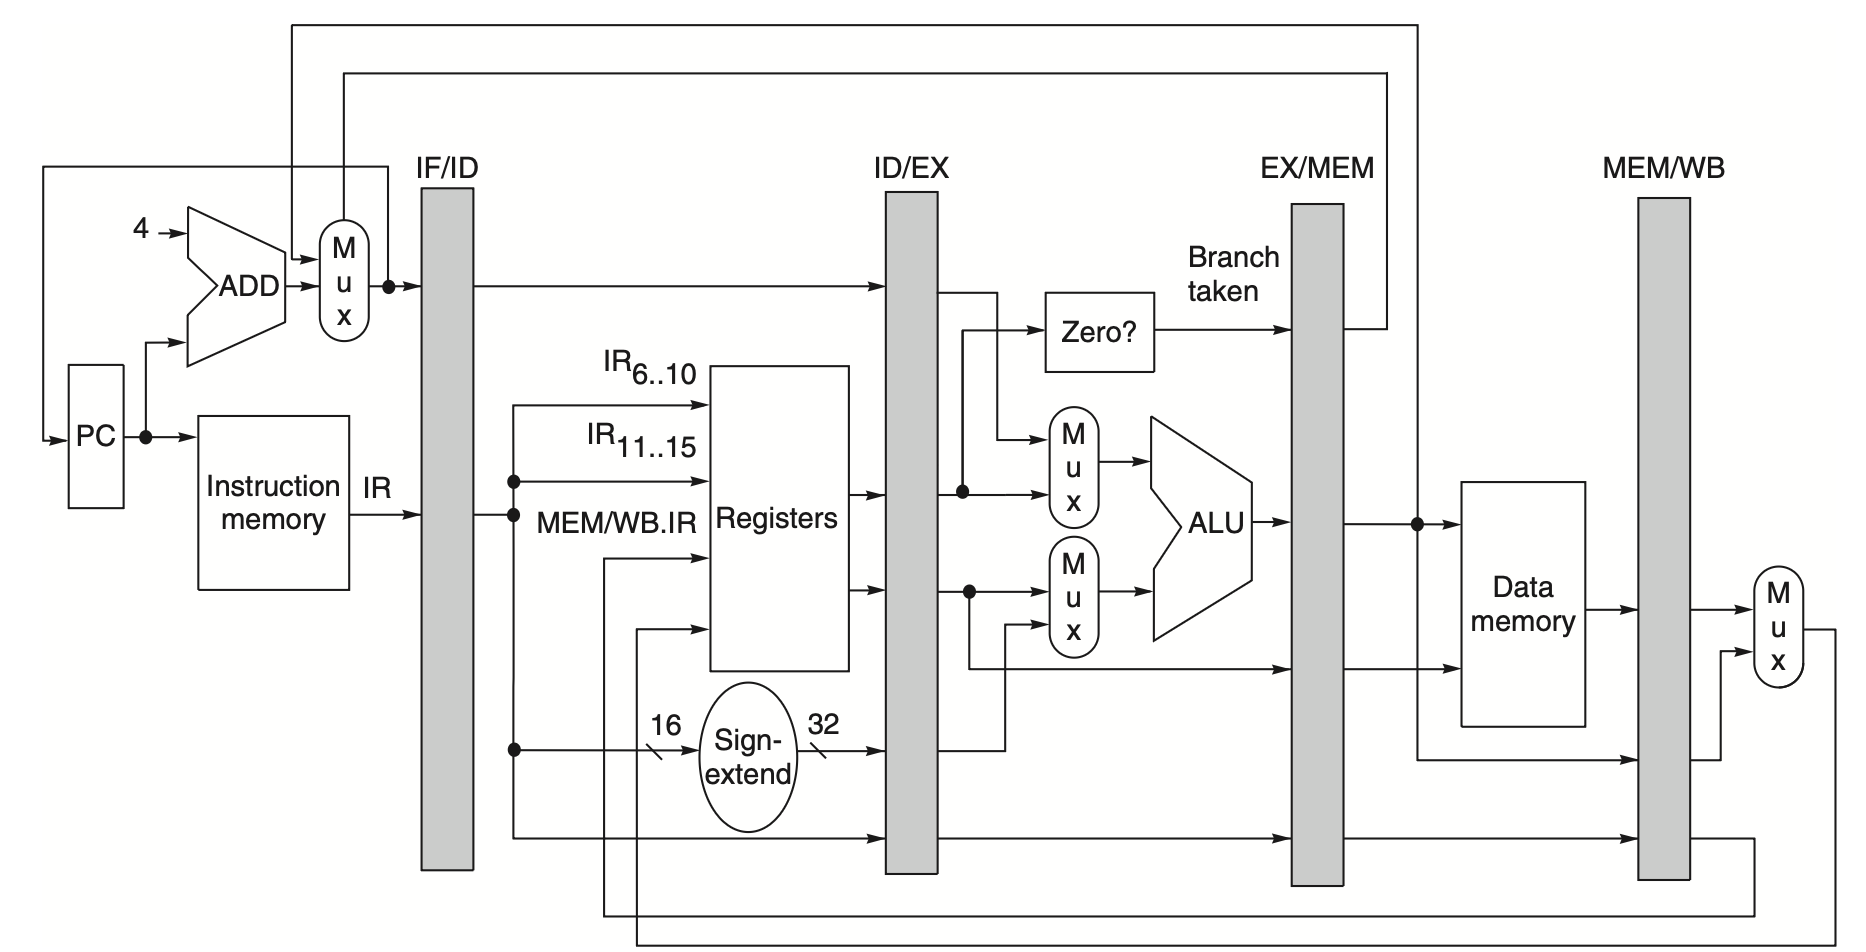
\includegraphics[width=\linewidth]{assets/figures/diag-36.png}
\diagramsource{H\&P Fig.~C.22, \hppage{C}{35} (image supplied by the note-taker); the same datapath as \nolinkurl{03-pipelining-lecture.pdf}, slide 26 (``5 Steps of MIPS Datapath'')}
\end{minipage}
\end{center}

Note: this is a \emph{data-stationary} control scheme -- each pipeline stage
locally decodes the control signals it needs from the instruction bits
carried along in the pipeline registers.

\subsubsection{Visualizing the pipeline (register read/write timing)}

\begin{center}\begin{minipage}{\linewidth}\centering
\begin{tikzpicture}[font=\scriptsize]
  \node[anchor=east,font=\scriptsize\itshape] at (-0.15,0.64) {cycle};
  \node at (0.525,0.64) {1};
  \node at (1.775,0.64) {2};
  \node at (3.025,0.64) {3};
  \node at (4.275,0.64) {4};
  \node at (5.525,0.64) {5};
  \node at (6.775,0.64) {6};
  \node at (8.025,0.64) {7};
  \node at (9.275,0.64) {8};
  \node[anchor=east] at (-0.15,0.000) {Instr 1};
  \draw (0.000,-0.275) rectangle (1.050,0.275);
  \node at (0.525,0.000) {Ifetch};
  \fill[black!25] (1.775,-0.275) rectangle (2.300,0.275);
  \draw (1.250,-0.275) rectangle (2.300,0.275);
  \node at (1.775,0.000) {Reg};
  \draw (2.500,-0.275) rectangle (3.550,0.275);
  \node at (3.025,0.000) {ALU};
  \draw (3.750,-0.275) rectangle (4.800,0.275);
  \node at (4.275,0.000) {DMem};
  \fill[black!25] (5.000,-0.275) rectangle (5.525,0.275);
  \draw (5.000,-0.275) rectangle (6.050,0.275);
  \node at (5.525,0.000) {Reg};
  \node[anchor=east] at (-0.15,-0.850) {Instr 2};
  \draw (1.250,-1.125) rectangle (2.300,-0.575);
  \node at (1.775,-0.850) {Ifetch};
  \fill[black!25] (3.025,-1.125) rectangle (3.550,-0.575);
  \draw (2.500,-1.125) rectangle (3.550,-0.575);
  \node at (3.025,-0.850) {Reg};
  \draw (3.750,-1.125) rectangle (4.800,-0.575);
  \node at (4.275,-0.850) {ALU};
  \draw (5.000,-1.125) rectangle (6.050,-0.575);
  \node at (5.525,-0.850) {DMem};
  \fill[black!25] (6.250,-1.125) rectangle (6.775,-0.575);
  \draw (6.250,-1.125) rectangle (7.300,-0.575);
  \node at (6.775,-0.850) {Reg};
  \node[anchor=east] at (-0.15,-1.700) {Instr 3};
  \draw (2.500,-1.975) rectangle (3.550,-1.425);
  \node at (3.025,-1.700) {Ifetch};
  \fill[black!25] (4.275,-1.975) rectangle (4.800,-1.425);
  \draw (3.750,-1.975) rectangle (4.800,-1.425);
  \node at (4.275,-1.700) {Reg};
  \draw (5.000,-1.975) rectangle (6.050,-1.425);
  \node at (5.525,-1.700) {ALU};
  \draw (6.250,-1.975) rectangle (7.300,-1.425);
  \node at (6.775,-1.700) {DMem};
  \fill[black!25] (7.500,-1.975) rectangle (8.025,-1.425);
  \draw (7.500,-1.975) rectangle (8.550,-1.425);
  \node at (8.025,-1.700) {Reg};
  \node[anchor=east] at (-0.15,-2.550) {Instr 4};
  \draw (3.750,-2.825) rectangle (4.800,-2.275);
  \node at (4.275,-2.550) {Ifetch};
  \fill[black!25] (5.525,-2.825) rectangle (6.050,-2.275);
  \draw (5.000,-2.825) rectangle (6.050,-2.275);
  \node at (5.525,-2.550) {Reg};
  \draw (6.250,-2.825) rectangle (7.300,-2.275);
  \node at (6.775,-2.550) {ALU};
  \draw (7.500,-2.825) rectangle (8.550,-2.275);
  \node at (8.025,-2.550) {DMem};
  \fill[black!25] (8.750,-2.825) rectangle (9.275,-2.275);
  \draw (8.750,-2.825) rectangle (9.800,-2.275);
  \node at (9.275,-2.550) {Reg};
  \fill[black!25] (0,-3.25) rectangle ++(0.25,0.25); \draw (0,-3.25) rectangle ++(0.5,0.25);
  \node[anchor=west] at (0.6,-3.125) {Reg in WB: written in the \emph{first} half of the cycle};
  \fill[black!25] (0.25,-3.65) rectangle ++(0.25,0.25); \draw (0,-3.65) rectangle ++(0.5,0.25);
  \node[anchor=west] at (0.6,-3.525) {Reg in ID: read in the \emph{second} half of the cycle};
\end{tikzpicture}
\diagramsource{\nolinkurl{03-pipelining-lecture.pdf}, slide 27 (``Visualizing Pipelining''); cf.\ H\&P Fig.~C.3, \hppage{C}{9}}
\end{minipage}
\end{center}

\begin{itemize}
  \item Read operand registers in the \textbf{second half} of the ID cycle.
  \item Write the destination register in the \textbf{first half} of the WB
  cycle.
\end{itemize}
This is an ideal integer in-order 5-stage pipeline.

\subsubsection{Pipelining performance example}

\begin{eg}[Pipelining a multi-cycle CPU]
For an unpipelined CPU: clock cycle $=1$ns; 4 cycles for ALU
operations/branches, 5 cycles for memory operations; instruction mix
$40\%/20\%/40\%$ (ALU/branch/memory). Pipelining adds 0.2ns to the clock
cycle.

\[
  \text{Non-pipelined avg.\ instr.\ time} = 1\text{ns}\times((40\%+20\%)\times4 + 40\%\times5) = 4.4\text{ns}
\]
\[
  \text{Pipelined avg.\ instr.\ time} = 1\text{ns} + 0.2\text{ns} = 1.2\text{ns}
\]
\[
  \text{Speedup} = \frac{4.4}{1.2} = 3.7 \times \text{ faster}
\]
\end{eg}

\subsection{Pipeline Hazards}
\label{sec:hazards}

\subsubsection{Three Kinds of Hazards}
\label{sec:hazard-types}

\begin{definition}[Pipeline hazards]
\textbf{Hazards} are situations in pipelining that prevent the next
instruction in the instruction stream from executing during its designated
clock cycle, possibly resulting in one or more \emph{stall} (wait) cycles.
Hazards increase CPI above 1 and are classified into three types:

\begin{itemize}
  \item \textbf{Structural hazards}: arise from hardware resource conflicts
  when available hardware cannot support all possible combinations of
  instructions.
  \item \textbf{Data hazards}: arise when an instruction depends on the
  result of a previous instruction in a way exposed by the overlapping of
  instructions in the pipeline.
  \item \textbf{Control hazards}: arise from the pipelining of conditional
  branches and other instructions that change the PC.
\end{itemize}\HPA{C}{\S C.2}{11}
\end{definition}

\begin{note}
An instruction ``issued later'' than instruction $x$
was issued after $x$ and is \emph{not as far along} in the pipeline. An
instruction ``issued earlier'' than $x$ was issued before $x$ and is
\emph{further along} in the pipeline.
\end{note}

\paragraph{Stalls and performance}

Stalls impede progress of a pipeline and cause deviation from 1
instruction/cycle.
\begin{prop}[CPI and speedup with stalls]
\[
  \mathrm{CPI}_{\text{pipelined}} = \text{Ideal CPI} + \text{Pipeline stall cycles per instruction} = 1 + \text{stall cycles/instr.}
\]
Ignoring overhead, assuming balanced stages:
\[
  \text{Speedup} = \frac{\mathrm{CPI}_{\text{unpipelined}}}{1 + \text{pipeline stall cycles per instruction}}
\]\HPA[13]{C}{\S C.2}{12}
\end{prop}

\subsubsection{Structural Hazards}
\label{sec:structural-hazards}

\begin{definition}[Structural hazard]
In pipelined machines, overlapped instruction execution requires pipelining
of functional units and duplication of resources so all possible
instruction combinations can be supported. If a \textbf{resource conflict}
arises because a hardware resource is required by more than one instruction
in a single cycle, and it cannot be accommodated, a \textbf{structural
hazard} occurs -- e.g.\ a pipelined machine with a single shared memory port
for instructions and data $\Rightarrow$ stall the pipeline for one cycle for
a memory data access.\HPA[15]{C}{\S C.2}{13}
\end{definition}

\paragraph{Example: single shared memory port}

\begin{center}\begin{minipage}{\linewidth}\centering
\begin{tikzpicture}[font=\scriptsize]
  \node[anchor=east,font=\scriptsize\itshape] at (-0.15,0.64) {cycle};
  \node at (0.525,0.64) {1};
  \node at (1.775,0.64) {2};
  \node at (3.025,0.64) {3};
  \node at (4.275,0.64) {4};
  \node at (5.525,0.64) {5};
  \node at (6.775,0.64) {6};
  \node at (8.025,0.64) {7};
  \node at (9.275,0.64) {8};
  \node at (10.525,0.64) {9};
  \node[anchor=east] at (-0.15,0.000) {Load};
  \draw (0.000,-0.275) rectangle (1.050,0.275);
  \node at (0.525,0.000) {Mem};
  \draw (1.250,-0.275) rectangle (2.300,0.275);
  \node at (1.775,0.000) {Reg};
  \draw (2.500,-0.275) rectangle (3.550,0.275);
  \node at (3.025,0.000) {ALU};
  \draw[very thick] (3.750,-0.275) rectangle (4.800,0.275);
  \node at (4.275,0.000) {DM};
  \draw (5.000,-0.275) rectangle (6.050,0.275);
  \node at (5.525,0.000) {Reg};
  \node[anchor=east] at (-0.15,-0.850) {Instr 1};
  \draw (1.250,-1.125) rectangle (2.300,-0.575);
  \node at (1.775,-0.850) {Mem};
  \draw (2.500,-1.125) rectangle (3.550,-0.575);
  \node at (3.025,-0.850) {Reg};
  \draw (3.750,-1.125) rectangle (4.800,-0.575);
  \node at (4.275,-0.850) {ALU};
  \draw (5.000,-1.125) rectangle (6.050,-0.575);
  \node at (5.525,-0.850) {DM};
  \draw (6.250,-1.125) rectangle (7.300,-0.575);
  \node at (6.775,-0.850) {Reg};
  \node[anchor=east] at (-0.15,-1.700) {Instr 2};
  \draw (2.500,-1.975) rectangle (3.550,-1.425);
  \node at (3.025,-1.700) {Mem};
  \draw (3.750,-1.975) rectangle (4.800,-1.425);
  \node at (4.275,-1.700) {Reg};
  \draw (5.000,-1.975) rectangle (6.050,-1.425);
  \node at (5.525,-1.700) {ALU};
  \draw (6.250,-1.975) rectangle (7.300,-1.425);
  \node at (6.775,-1.700) {DM};
  \draw (7.500,-1.975) rectangle (8.550,-1.425);
  \node at (8.025,-1.700) {Reg};
  \node[anchor=east] at (-0.15,-2.550) {Instr 3};
  \draw[very thick] (3.750,-2.825) rectangle (4.800,-2.275);
  \node at (4.275,-2.550) {Mem};
  \draw (5.000,-2.825) rectangle (6.050,-2.275);
  \node at (5.525,-2.550) {Reg};
  \draw (6.250,-2.825) rectangle (7.300,-2.275);
  \node at (6.775,-2.550) {ALU};
  \draw (7.500,-2.825) rectangle (8.550,-2.275);
  \node at (8.025,-2.550) {DM};
  \draw (8.750,-2.825) rectangle (9.800,-2.275);
  \node at (9.275,-2.550) {Reg};
  \node[anchor=east] at (-0.15,-3.400) {Instr 4};
  \draw (5.000,-3.675) rectangle (6.050,-3.125);
  \node at (5.525,-3.400) {Mem};
  \draw (6.250,-3.675) rectangle (7.300,-3.125);
  \node at (6.775,-3.400) {Reg};
  \draw (7.500,-3.675) rectangle (8.550,-3.125);
  \node at (8.025,-3.400) {ALU};
  \draw (8.750,-3.675) rectangle (9.800,-3.125);
  \node at (9.275,-3.400) {DM};
  \draw (10.000,-3.675) rectangle (11.050,-3.125);
  \node at (10.525,-3.400) {Reg};
  \draw[dashed,rounded corners=6pt] (3.70,0.45) rectangle (4.95,-2.95);
  \node[anchor=north west,font=\scriptsize] at (0,-3.85) {cycle 4: the Load's data access (DM) and Instr 3's instruction fetch (Mem) both need the one memory port};
\end{tikzpicture}
\diagramsource{\nolinkurl{03-pipelining-lecture.pdf}, slide 33 (``An example of a structural hazard''); cf.\ H\&P Fig.~C.4, \hppage{C}{14}}
\end{minipage}
\end{center}

\textbf{Resolution: stall (insert a bubble/NOP).}

\begin{center}\begin{minipage}{\linewidth}\centering
\begin{tikzpicture}[font=\scriptsize]
  \node[anchor=east,font=\scriptsize\itshape] at (-0.15,0.64) {cycle};
  \node at (0.500,0.64) {1};
  \node at (1.700,0.64) {2};
  \node at (2.900,0.64) {3};
  \node at (4.100,0.64) {4};
  \node at (5.300,0.64) {5};
  \node at (6.500,0.64) {6};
  \node at (7.700,0.64) {7};
  \node at (8.900,0.64) {8};
  \node at (10.100,0.64) {9};
  \node[anchor=east] at (-0.15,0.000) {Load};
  \draw (0.000,-0.275) rectangle (1.000,0.275);
  \node at (0.500,0.000) {Mem};
  \draw (1.200,-0.275) rectangle (2.200,0.275);
  \node at (1.700,0.000) {Reg};
  \draw (2.400,-0.275) rectangle (3.400,0.275);
  \node at (2.900,0.000) {ALU};
  \draw (3.600,-0.275) rectangle (4.600,0.275);
  \node at (4.100,0.000) {DM};
  \draw (4.800,-0.275) rectangle (5.800,0.275);
  \node at (5.300,0.000) {Reg};
  \node[anchor=east] at (-0.15,-0.850) {Instr 1};
  \draw (1.200,-1.125) rectangle (2.200,-0.575);
  \node at (1.700,-0.850) {Mem};
  \draw (2.400,-1.125) rectangle (3.400,-0.575);
  \node at (2.900,-0.850) {Reg};
  \draw (3.600,-1.125) rectangle (4.600,-0.575);
  \node at (4.100,-0.850) {ALU};
  \draw (4.800,-1.125) rectangle (5.800,-0.575);
  \node at (5.300,-0.850) {DM};
  \draw (6.000,-1.125) rectangle (7.000,-0.575);
  \node at (6.500,-0.850) {Reg};
  \node[anchor=east] at (-0.15,-1.700) {Instr 2};
  \draw (2.400,-1.975) rectangle (3.400,-1.425);
  \node at (2.900,-1.700) {Mem};
  \draw (3.600,-1.975) rectangle (4.600,-1.425);
  \node at (4.100,-1.700) {Reg};
  \draw (4.800,-1.975) rectangle (5.800,-1.425);
  \node at (5.300,-1.700) {ALU};
  \draw (6.000,-1.975) rectangle (7.000,-1.425);
  \node at (6.500,-1.700) {DM};
  \draw (7.200,-1.975) rectangle (8.200,-1.425);
  \node at (7.700,-1.700) {Reg};
  \node[anchor=east] at (-0.15,-2.550) {\emph{stall}};
  \draw[dashed,rounded corners=4pt] (3.650,-2.785) rectangle (4.550,-2.315);
  \node[font=\tiny\itshape] at (4.100,-2.550) {bubble};
  \draw[dashed,rounded corners=4pt] (4.850,-2.785) rectangle (5.750,-2.315);
  \node[font=\tiny\itshape] at (5.300,-2.550) {bubble};
  \draw[dashed,rounded corners=4pt] (6.050,-2.785) rectangle (6.950,-2.315);
  \node[font=\tiny\itshape] at (6.500,-2.550) {bubble};
  \draw[dashed,rounded corners=4pt] (7.250,-2.785) rectangle (8.150,-2.315);
  \node[font=\tiny\itshape] at (7.700,-2.550) {bubble};
  \draw[dashed,rounded corners=4pt] (8.450,-2.785) rectangle (9.350,-2.315);
  \node[font=\tiny\itshape] at (8.900,-2.550) {bubble};
  \node[anchor=east] at (-0.15,-3.400) {Instr 3};
  \draw (4.800,-3.675) rectangle (5.800,-3.125);
  \node at (5.300,-3.400) {Mem};
  \draw (6.000,-3.675) rectangle (7.000,-3.125);
  \node at (6.500,-3.400) {Reg};
  \draw (7.200,-3.675) rectangle (8.200,-3.125);
  \node at (7.700,-3.400) {ALU};
  \draw (8.400,-3.675) rectangle (9.400,-3.125);
  \node at (8.900,-3.400) {DM};
  \draw (9.600,-3.675) rectangle (10.600,-3.125);
  \node at (10.100,-3.400) {Reg};

\end{tikzpicture}
\diagramsource{\nolinkurl{03-pipelining-lecture.pdf}, slide 34 (``How is it resolved?''); cf.\ H\&P Fig.~C.5, \hppage{C}{15}}
\end{minipage}
\end{center}

\paragraph{Structural hazard: numeric example}

\begin{eg}[Is a structural hazard worth it?]
Given data references are $40\%$ of a program, ideal pipelined CPI $=1$. A
machine with a data-memory structural hazard needs 1 stall cycle per data
reference, but its clock rate is $1.05\times$ higher than the ideal
machine:
\[
  \text{Avg.\ instr.\ time} = (1+0.4\times1)\times\frac{\text{Clock}_{\text{ideal}}}{1.05} = 1.3\times \text{Clock}_{\text{ideal}}
\]
$\Rightarrow$ the machine \emph{without} the hazard is still better ($1.3 >
1$).
\end{eg}

\begin{remark}
\textbf{Remember the common case!} All else equal, a machine without
structural hazards always has lower CPI, but sometimes it is cheaper (in
hardware) to allow a hazard than to eliminate it -- weigh HW cost of
pipelining/duplicating a unit against how often the hazard actually occurs.
\end{remark}

\subsubsection{Data Hazards}
\label{sec:data-hazards}

\begin{definition}[Data hazard]
Data hazards occur when the pipeline changes the order of read/write
accesses to operands compared to the original sequential order, potentially
causing \textbf{incorrect execution}. One or more instructions may need to
stall to ensure correctness.\HPA{C}{\S C.2}{15}
\end{definition}

\begin{eg}[RAW on R1]
\leavevmode
\begin{lstlisting}
ADD R1, R2, R3
SUB R4, R1, R5
AND R6, R1, R7
OR  R8, R1, R9
XOR R10, R1, R11
\end{lstlisting}
All instructions after \texttt{ADD} use its result (\texttt{R1}); \texttt{SUB}
and \texttt{AND} would need to stall for correct execution without
forwarding.
\end{eg}

\paragraph{Data Hazard Classification}

\begin{definition}[RAW, WAW, WAR]
Given two instructions $I$, $J$, with $I$ occurring before $J$ in program
order:

\begin{itemize}
  \item \textbf{RAW} (read after write) -- \emph{true data dependence}: $J$
  tries to read a source before $I$ writes it, so $J$ incorrectly gets the
  old value.
  \item \textbf{WAW} (write after write) -- \emph{name dependence}: $J$
  tries to write an operand before it is written by $I$; the writes end up
  performed in the wrong order.
  \item \textbf{WAR} (write after read) -- \emph{name dependence}: $J$
  tries to write a destination before it is read by $I$, so $I$ incorrectly
  gets the new value.
  \item \textbf{RAR} (read after read): \emph{not} a hazard.
\end{itemize}\HP{\S3.1, Data Hazards}{153}
\end{definition}

\begin{center}\begin{minipage}{\linewidth}\centering
\begin{tikzpicture}[font=\small]
  \draw[-{Latex}] (-1.6,1.3) -- (-1.6,0) node[midway,left,font=\scriptsize,align=right] {program\\order};
  \begin{scope}[xshift=0.00cm]
  \node[draw,minimum width=1.9cm] (I) at (0,1.3) {$I$ (Write)};
  \node[draw,minimum width=1.9cm] (J) at (0,0) {$J$ (Read)};
  \node[draw,align=center] (S) at (2.7,0.65) {Shared\\operand};
  \draw[-{Latex}] (I.east) -- (S.north west);
  \draw[-{Latex}] (S.south west) -- (J.east);
  \node[font=\small\bfseries,align=center] at (1.35,-0.75) {RAW (true dependence)};
  \end{scope}
  \begin{scope}[xshift=6.20cm]
  \node[draw,minimum width=1.9cm] (I) at (0,1.3) {$I$ (Read)};
  \node[draw,minimum width=1.9cm] (J) at (0,0) {$J$ (Write)};
  \node[draw,align=center] (S) at (2.7,0.65) {Shared\\operand};
  \draw[-{Latex}] (S.north west) -- (I.east);
  \draw[-{Latex}] (J.east) -- (S.south west);
  \node[font=\small\bfseries,align=center] at (1.35,-0.75) {WAR (name dependence)};
  \end{scope}
\end{tikzpicture}
\diagramsource{\nolinkurl{03-pipelining-lecture.pdf}, slide 45 (``Data Hazard Classification'') (RAW, WAR)}
\end{minipage}
\end{center}

\begin{center}\begin{minipage}{\linewidth}\centering
\begin{tikzpicture}[font=\small]
  \draw[-{Latex}] (-1.6,1.3) -- (-1.6,0) node[midway,left,font=\scriptsize,align=right] {program\\order};
  \begin{scope}[xshift=0.00cm]
  \node[draw,minimum width=1.9cm] (I) at (0,1.3) {$I$ (Write)};
  \node[draw,minimum width=1.9cm] (J) at (0,0) {$J$ (Write)};
  \node[draw,align=center] (S) at (2.7,0.65) {Shared\\operand};
  \draw[-{Latex}] (I.east) -- (S.north west);
  \draw[-{Latex}] (J.east) -- (S.south west);
  \node[font=\small\bfseries,align=center] at (1.35,-0.75) {WAW (name dependence)};
  \end{scope}
  \begin{scope}[xshift=6.20cm]
  \node[draw,minimum width=1.9cm] (I) at (0,1.3) {$I$ (Read)};
  \node[draw,minimum width=1.9cm] (J) at (0,0) {$J$ (Read)};
  \node[draw,align=center] (S) at (2.7,0.65) {Shared\\operand};
  \draw[-{Latex}] (S.north west) -- (I.east);
  \draw[-{Latex}] (S.south west) -- (J.east);
  \node[font=\small\bfseries,align=center] at (1.35,-0.75) {RAR (\emph{not} a hazard)};
  \end{scope}
\end{tikzpicture}
\diagramsource{\nolinkurl{03-pipelining-lecture.pdf}, slide 45 (``Data Hazard Classification'') (WAW, RAR)}
\end{minipage}
\end{center}

\begin{itemize}
  \item \textbf{RAW example:} \texttt{i: ADD R1,R2,R3} \quad
        \texttt{j: SUB R4,R1,R6}
  \item \textbf{WAW example:} \texttt{i: SUB R1,R4,R3} \quad
        \texttt{j: ADD R1,R2,R3}
  \item \textbf{WAR example:} \texttt{i: SUB R4,R1,R3} \quad
        \texttt{j: ADD R1,R2,R3}
\end{itemize}
\begin{remark}
RAW and WAW can be resolved with stalling or forwarding; WAR does not occur
in the simple MIPS pipeline because reads happen early (ID) and writes late
(WB) in program order, so instructions never write before an earlier one has
read (only relevant for pipelines that reorder execution).
\end{remark}

\paragraph{Data hazard on R1 (visualized)}

\begin{center}\begin{minipage}{\linewidth}\centering
\begin{tikzpicture}[font=\scriptsize]
  \node[anchor=east,font=\scriptsize\itshape] at (-0.15,0.64) {cycle};
  \node at (0.525,0.64) {1};
  \node at (1.775,0.64) {2};
  \node at (3.025,0.64) {3};
  \node at (4.275,0.64) {4};
  \node at (5.525,0.64) {5};
  \node at (6.775,0.64) {6};
  \node at (8.025,0.64) {7};
  \node at (9.275,0.64) {8};
  \node at (10.525,0.64) {9};
  \node[anchor=east] at (-0.15,0.000) {\texttt{add r1,r2,r3}};
  \draw (0.000,-0.275) rectangle (1.050,0.275);
  \node at (0.525,0.000) {Ifetch};
  \draw (1.250,-0.275) rectangle (2.300,0.275);
  \node at (1.775,0.000) {Reg};
  \draw (2.500,-0.275) rectangle (3.550,0.275);
  \node at (3.025,0.000) {ALU};
  \draw (3.750,-0.275) rectangle (4.800,0.275);
  \node at (4.275,0.000) {DMem};
  \draw (5.000,-0.275) rectangle (6.050,0.275);
  \node at (5.525,0.000) {Reg};
  \node[anchor=east] at (-0.15,-0.850) {\texttt{sub r4,r1,r3}};
  \draw (1.250,-1.125) rectangle (2.300,-0.575);
  \node at (1.775,-0.850) {Ifetch};
  \draw (2.500,-1.125) rectangle (3.550,-0.575);
  \node at (3.025,-0.850) {Reg};
  \draw (3.750,-1.125) rectangle (4.800,-0.575);
  \node at (4.275,-0.850) {ALU};
  \draw (5.000,-1.125) rectangle (6.050,-0.575);
  \node at (5.525,-0.850) {DMem};
  \draw (6.250,-1.125) rectangle (7.300,-0.575);
  \node at (6.775,-0.850) {Reg};
  \node[anchor=east] at (-0.15,-1.700) {\texttt{and r6,r1,r7}};
  \draw (2.500,-1.975) rectangle (3.550,-1.425);
  \node at (3.025,-1.700) {Ifetch};
  \draw (3.750,-1.975) rectangle (4.800,-1.425);
  \node at (4.275,-1.700) {Reg};
  \draw (5.000,-1.975) rectangle (6.050,-1.425);
  \node at (5.525,-1.700) {ALU};
  \draw (6.250,-1.975) rectangle (7.300,-1.425);
  \node at (6.775,-1.700) {DMem};
  \draw (7.500,-1.975) rectangle (8.550,-1.425);
  \node at (8.025,-1.700) {Reg};
  \node[anchor=east] at (-0.15,-2.550) {\texttt{or\ \ r8,r1,r9}};
  \draw (3.750,-2.825) rectangle (4.800,-2.275);
  \node at (4.275,-2.550) {Ifetch};
  \draw (5.000,-2.825) rectangle (6.050,-2.275);
  \node at (5.525,-2.550) {Reg};
  \draw (6.250,-2.825) rectangle (7.300,-2.275);
  \node at (6.775,-2.550) {ALU};
  \draw (7.500,-2.825) rectangle (8.550,-2.275);
  \node at (8.025,-2.550) {DMem};
  \draw (8.750,-2.825) rectangle (9.800,-2.275);
  \node at (9.275,-2.550) {Reg};
  \node[anchor=east] at (-0.15,-3.400) {\texttt{xor r10,r1,r11}};
  \draw (5.000,-3.675) rectangle (6.050,-3.125);
  \node at (5.525,-3.400) {Ifetch};
  \draw (6.250,-3.675) rectangle (7.300,-3.125);
  \node at (6.775,-3.400) {Reg};
  \draw (7.500,-3.675) rectangle (8.550,-3.125);
  \node at (8.025,-3.400) {ALU};
  \draw (8.750,-3.675) rectangle (9.800,-3.125);
  \node at (9.275,-3.400) {DMem};
  \draw (10.000,-3.675) rectangle (11.050,-3.125);
  \node at (10.525,-3.400) {Reg};
  \draw[-{Latex[length=2mm]},thick,solid] (4.900,-0.275) -- (3.025,-0.575);
  \draw[-{Latex[length=2mm]},thick,solid] (4.900,-0.275) -- (4.900,-1.275) -- (4.275,-1.425);
  \draw[-{Latex[length=2mm]},thick,dashed] (6.150,-0.275) -- (6.150,-2.125) -- (5.525,-2.275);
  \draw[-{Latex[length=2mm]},thick,dashed] (6.150,-0.275) -- (6.150,-2.975) -- (6.775,-3.125);
  \draw[thick,-{Latex[length=2mm]}] (0,-4.1) -- (0.7,-4.1); \node[anchor=west] at (0.8,-4.1) {needed before \texttt{add} writes \texttt{r1}: hazard};
  \draw[thick,dashed,-{Latex[length=2mm]}] (0,-4.5) -- (0.7,-4.5); \node[anchor=west] at (0.8,-4.5) {read after the write (WB first half): no hazard};
\end{tikzpicture}
\diagramsource{\nolinkurl{03-pipelining-lecture.pdf}, slide 39 (``Data Hazard on R1''); cf.\ H\&P Fig.~C.6, \hppage{C}{17}}
\end{minipage}
\end{center}
Without forwarding, \texttt{add}'s result is only available (written back)
after its WB stage, but \texttt{sub} needs \texttt{r1} in its ID stage one
cycle earlier -- a RAW hazard.

\subsubsection{Minimizing Data Hazard Stalls by Forwarding}
\label{sec:forwarding}

\begin{definition}[Forwarding]
\textbf{Forwarding} (a.k.a.\ \emph{register bypassing} or
\emph{short-circuiting}) is a hardware-based technique used to eliminate or
minimize data-hazard stalls. The result of an instruction is copied directly
from where it is produced (ALU output, memory read port, etc.) to where a
subsequent instruction needs it (ALU input register, memory write port,
etc.), \emph{without} waiting for it to be written to and re-read from the
register file.\HPA[18]{C}{\S C.2}{16}
\end{definition}

In the MIPS integer pipeline with forwarding:
\begin{itemize}
  \item The \textbf{ALU result} from the EX/MEM register may be forwarded
  back to the ALU input latches instead of the register value read in ID.
  \item The \textbf{Data Memory result} from the MEM/WB register may also be
  forwarded to the ALU input latches.
  \item If the forwarding hardware detects that a previous ALU operation
  will write the register that is a source for the current ALU operation,
  control logic selects the forwarded result as the ALU input instead of the
  value read from the register file.
\end{itemize}

\paragraph{Datapath modified for forwarding}

\begin{center}\begin{minipage}{\linewidth}\centering
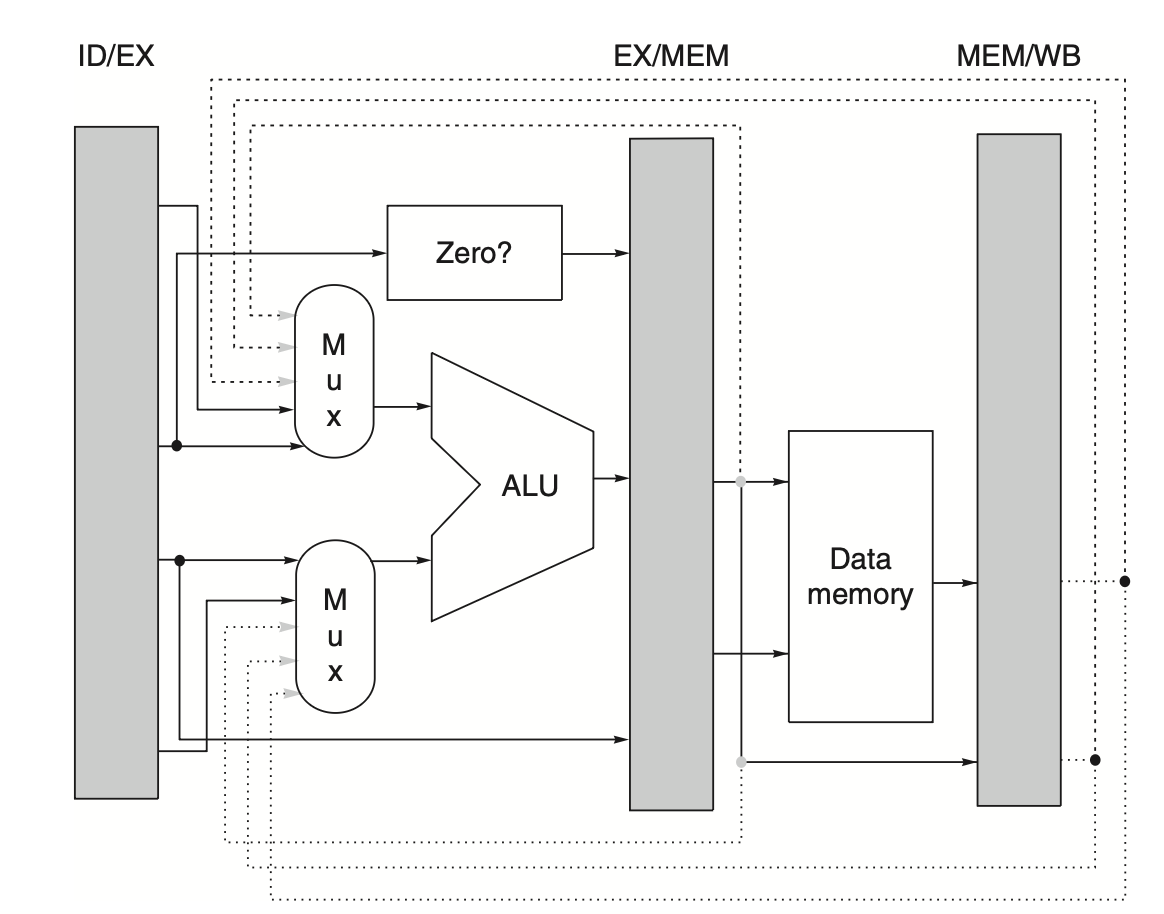
\includegraphics[width=0.7\linewidth]{assets/figures/diag-43.png}
\diagramsource{H\&P Fig.~C.27, \hppage{C}{41} (image supplied by the note-taker; dotted lines are the forwarding paths); cf.\ \nolinkurl{03-pipelining-lecture.pdf}, slide 41 (``HW Change for Forwarding'')}
\end{minipage}
\end{center}
Red paths show the EX/MEM $\to$ ALU-input and MEM/WB $\to$ ALU-input
forwarding routes, plus the normal write-back path to the register file.

\paragraph{Forwarding to avoid the RAW hazard}

\begin{center}\begin{minipage}{\linewidth}\centering
\begin{tikzpicture}[font=\scriptsize]
  \node[anchor=east,font=\scriptsize\itshape] at (-0.15,0.64) {cycle};
  \node at (0.525,0.64) {1};
  \node at (1.775,0.64) {2};
  \node at (3.025,0.64) {3};
  \node at (4.275,0.64) {4};
  \node at (5.525,0.64) {5};
  \node at (6.775,0.64) {6};
  \node at (8.025,0.64) {7};
  \node at (9.275,0.64) {8};
  \node at (10.525,0.64) {9};
  \node[anchor=east] at (-0.15,0.000) {\texttt{add r1,r2,r3}};
  \draw (0.000,-0.275) rectangle (1.050,0.275);
  \node at (0.525,0.000) {Ifetch};
  \draw (1.250,-0.275) rectangle (2.300,0.275);
  \node at (1.775,0.000) {Reg};
  \draw (2.500,-0.275) rectangle (3.550,0.275);
  \node at (3.025,0.000) {ALU};
  \draw (3.750,-0.275) rectangle (4.800,0.275);
  \node at (4.275,0.000) {DMem};
  \draw (5.000,-0.275) rectangle (6.050,0.275);
  \node at (5.525,0.000) {Reg};
  \node[anchor=east] at (-0.15,-0.850) {\texttt{sub r4,r1,r3}};
  \draw (1.250,-1.125) rectangle (2.300,-0.575);
  \node at (1.775,-0.850) {Ifetch};
  \draw (2.500,-1.125) rectangle (3.550,-0.575);
  \node at (3.025,-0.850) {Reg};
  \draw (3.750,-1.125) rectangle (4.800,-0.575);
  \node at (4.275,-0.850) {ALU};
  \draw (5.000,-1.125) rectangle (6.050,-0.575);
  \node at (5.525,-0.850) {DMem};
  \draw (6.250,-1.125) rectangle (7.300,-0.575);
  \node at (6.775,-0.850) {Reg};
  \node[anchor=east] at (-0.15,-1.700) {\texttt{and r6,r1,r7}};
  \draw (2.500,-1.975) rectangle (3.550,-1.425);
  \node at (3.025,-1.700) {Ifetch};
  \draw (3.750,-1.975) rectangle (4.800,-1.425);
  \node at (4.275,-1.700) {Reg};
  \draw (5.000,-1.975) rectangle (6.050,-1.425);
  \node at (5.525,-1.700) {ALU};
  \draw (6.250,-1.975) rectangle (7.300,-1.425);
  \node at (6.775,-1.700) {DMem};
  \draw (7.500,-1.975) rectangle (8.550,-1.425);
  \node at (8.025,-1.700) {Reg};
  \node[anchor=east] at (-0.15,-2.550) {\texttt{or\ \ r8,r1,r9}};
  \draw (3.750,-2.825) rectangle (4.800,-2.275);
  \node at (4.275,-2.550) {Ifetch};
  \draw (5.000,-2.825) rectangle (6.050,-2.275);
  \node at (5.525,-2.550) {Reg};
  \draw (6.250,-2.825) rectangle (7.300,-2.275);
  \node at (6.775,-2.550) {ALU};
  \draw (7.500,-2.825) rectangle (8.550,-2.275);
  \node at (8.025,-2.550) {DMem};
  \draw (8.750,-2.825) rectangle (9.800,-2.275);
  \node at (9.275,-2.550) {Reg};
  \node[anchor=east] at (-0.15,-3.400) {\texttt{xor r10,r1,r11}};
  \draw (5.000,-3.675) rectangle (6.050,-3.125);
  \node at (5.525,-3.400) {Ifetch};
  \draw (6.250,-3.675) rectangle (7.300,-3.125);
  \node at (6.775,-3.400) {Reg};
  \draw (7.500,-3.675) rectangle (8.550,-3.125);
  \node at (8.025,-3.400) {ALU};
  \draw (8.750,-3.675) rectangle (9.800,-3.125);
  \node at (9.275,-3.400) {DMem};
  \draw (10.000,-3.675) rectangle (11.050,-3.125);
  \node at (10.525,-3.400) {Reg};
  \draw[-{Latex[length=2mm]},thick,solid] (3.650,-0.275) -- (4.275,-0.575);
  \draw[-{Latex[length=2mm]},thick,solid] (4.900,-0.275) -- (4.900,-1.275) -- (5.525,-1.425);
  \draw[-{Latex[length=2mm]},thick,dashed] (6.150,-0.275) -- (6.150,-2.125) -- (5.525,-2.275);
  \draw[thick,-{Latex[length=2mm]}] (0,-4.1) -- (0.7,-4.1); \node[anchor=west] at (0.8,-4.1) {forwarded from EX/MEM or MEM/WB to the ALU};
  \draw[thick,dashed,-{Latex[length=2mm]}] (0,-4.5) -- (0.7,-4.5); \node[anchor=west] at (0.8,-4.5) {through the register file (write, then read)};
\end{tikzpicture}
\diagramsource{\nolinkurl{03-pipelining-lecture.pdf}, slide 42 (``Forwarding to Avoid Data Hazard''); cf.\ H\&P Fig.~C.7, \hppage{C}{18}}
\end{minipage}
\end{center}
The ALU result of \texttt{add} is forwarded directly into the ALU input of
\texttt{sub} in the very next cycle -- no stall needed.

\paragraph{Forwarding to avoid an LW--SW data hazard}

\begin{lstlisting}
add r1,r2,r3
lw  r4,0(r1)
sw  r4,12(r1)
or  r8,r6,r9
xor r10,r9,r11
\end{lstlisting}
\begin{note}
The value loaded by \texttt{lw} into \texttt{r4} is forwarded from the
MEM/WB register directly to the \texttt{sw}'s store-data input, avoiding a
stall.
\end{note}

\subsubsection{Data Hazards Even With Forwarding: The Load-Use Hazard}
\label{sec:load-use}

\begin{remark}
Some hazards \emph{cannot} be resolved by forwarding alone, because the
needed value is not produced early enough.
\end{remark}

\begin{lstlisting}
lw  r1, 0(r2)
sub r4, r1, r6
and r6, r1, r7
or  r8, r1, r9
\end{lstlisting}

\texttt{lw} produces \texttt{r1} at the \emph{end of its MEM stage} (cycle
4), but \texttt{sub} needs it as an ALU input at the \emph{start of its EX
stage} (cycle 3) -- one cycle too early even with forwarding. A single
stall cycle (bubble) must be inserted:

\begin{center}\begin{minipage}{\linewidth}\centering
\begin{tikzpicture}[font=\scriptsize]
  \node[anchor=east,font=\scriptsize\itshape] at (-0.15,0.64) {cycle};
  \node at (0.525,0.64) {1};
  \node at (1.775,0.64) {2};
  \node at (3.025,0.64) {3};
  \node at (4.275,0.64) {4};
  \node at (5.525,0.64) {5};
  \node at (6.775,0.64) {6};
  \node at (8.025,0.64) {7};
  \node at (9.275,0.64) {8};
  \node at (10.525,0.64) {9};
  \node[anchor=east] at (-0.15,0.000) {\texttt{lw\ \ r1,0(r2)}};
  \draw (0.000,-0.275) rectangle (1.050,0.275);
  \node at (0.525,0.000) {Ifetch};
  \draw (1.250,-0.275) rectangle (2.300,0.275);
  \node at (1.775,0.000) {Reg};
  \draw (2.500,-0.275) rectangle (3.550,0.275);
  \node at (3.025,0.000) {ALU};
  \draw (3.750,-0.275) rectangle (4.800,0.275);
  \node at (4.275,0.000) {DMem};
  \draw (5.000,-0.275) rectangle (6.050,0.275);
  \node at (5.525,0.000) {Reg};
  \node[anchor=east] at (-0.15,-0.850) {\texttt{sub r4,r1,r6}};
  \draw (1.250,-1.125) rectangle (2.300,-0.575);
  \node at (1.775,-0.850) {Ifetch};
  \draw (2.500,-1.125) rectangle (3.550,-0.575);
  \node at (3.025,-0.850) {Reg};
  \draw[dashed,rounded corners=4pt] (3.800,-1.085) rectangle (4.750,-0.615);
  \node[font=\tiny\itshape] at (4.275,-0.850) {bubble};
  \draw (5.000,-1.125) rectangle (6.050,-0.575);
  \node at (5.525,-0.850) {ALU};
  \draw (6.250,-1.125) rectangle (7.300,-0.575);
  \node at (6.775,-0.850) {DMem};
  \draw (7.500,-1.125) rectangle (8.550,-0.575);
  \node at (8.025,-0.850) {Reg};
  \node[anchor=east] at (-0.15,-1.700) {\texttt{and r6,r1,r7}};
  \draw (2.500,-1.975) rectangle (3.550,-1.425);
  \node at (3.025,-1.700) {Ifetch};
  \draw[dashed,rounded corners=4pt] (3.800,-1.935) rectangle (4.750,-1.465);
  \node[font=\tiny\itshape] at (4.275,-1.700) {bubble};
  \draw (5.000,-1.975) rectangle (6.050,-1.425);
  \node at (5.525,-1.700) {Reg};
  \draw (6.250,-1.975) rectangle (7.300,-1.425);
  \node at (6.775,-1.700) {ALU};
  \draw (7.500,-1.975) rectangle (8.550,-1.425);
  \node at (8.025,-1.700) {DMem};
  \draw (8.750,-1.975) rectangle (9.800,-1.425);
  \node at (9.275,-1.700) {Reg};
  \node[anchor=east] at (-0.15,-2.550) {\texttt{or\ \ r8,r1,r9}};
  \draw[dashed,rounded corners=4pt] (3.800,-2.785) rectangle (4.750,-2.315);
  \node[font=\tiny\itshape] at (4.275,-2.550) {bubble};
  \draw (5.000,-2.825) rectangle (6.050,-2.275);
  \node at (5.525,-2.550) {Ifetch};
  \draw (6.250,-2.825) rectangle (7.300,-2.275);
  \node at (6.775,-2.550) {Reg};
  \draw (7.500,-2.825) rectangle (8.550,-2.275);
  \node at (8.025,-2.550) {ALU};
  \draw (8.750,-2.825) rectangle (9.800,-2.275);
  \node at (9.275,-2.550) {DMem};
  \draw[-{Latex[length=2mm]},thick,solid] (4.900,-0.275) -- (5.525,-0.575);
  \draw[-{Latex[length=2mm]},thick,dashed] (6.150,-0.275) -- (6.150,-1.275) -- (5.525,-1.425);
  \draw[thick,-{Latex[length=2mm]}] (0,-3.3) -- (0.7,-3.3); \node[anchor=west] at (0.8,-3.3) {MEM/WB $\to$ ALU after a one-cycle stall};
  \draw[thick,dashed,-{Latex[length=2mm]}] (0,-3.7) -- (0.7,-3.7); \node[anchor=west] at (0.8,-3.7) {through the register file};
\end{tikzpicture}
\diagramsource{\nolinkurl{03-pipelining-lecture.pdf}, slide 51 (``Data Hazard Even with Forwarding'') (slide 50 without the bubble); cf.\ H\&P Fig.~C.9, \hppage{C}{20}}
\end{minipage}
\end{center}

\paragraph{Hardware pipeline interlocks}

\begin{definition}[Pipeline interlock]
A \textbf{hardware pipeline interlock} detects a data hazard and stalls the
pipeline until the hazard clears. The CPI for the stalled instruction
increases by the length of the stall.\HPA[21]{C}{\S C.2}{19}
\end{definition}

\begin{lstlisting}[caption={No hazard (ideal)}]
              c1    c2    c3    c4    c5    c6    c7    c8    c9
LW  R1,0(R1)  IF    ID    EX    MEM   WB
SUB R4,R1,R5        IF    ID    EX    MEM   WB
AND R6,R1,R7              IF    ID    EX    MEM   WB
OR  R8,R1,R9                    IF    ID    EX    MEM   WB
\end{lstlisting}
\begin{lstlisting}[caption={Load-use hazard: interlock inserts one stall, then forwards}]
              c1    c2    c3    c4    c5    c6    c7    c8    c9
LW  R1,0(R1)  IF    ID    EX    MEM   WB
SUB R4,R1,R5        IF    ID    stall EX    MEM   WB
AND R6,R1,R7              IF    stall ID    EX    MEM   WB
OR  R8,R1,R9                    stall IF    ID    EX    MEM   WB
\end{lstlisting}

\paragraph{Data hazards and the compiler}

\begin{definition}[Pipeline (instruction) scheduling]
The compiler can help eliminate some hazard-induced stalls: it should avoid
generating a \texttt{LOAD} instruction immediately followed by an
instruction that uses the load's destination register. This technique is
called \textbf{pipeline / instruction scheduling}.
\end{definition}

\begin{center}
\begin{tabular}{@{}p{3.4cm}p{4.3cm}p{5.6cm}@{}}
\toprule
Situation & Example & Action \\
\midrule
No dependence &
\texttt{LW R1,45(R2)}\newline\texttt{ADD R5,R6,R7}\newline\texttt{SUB R8,R6,R7}\newline\texttt{OR R9,R6,R7} &
No hazard possible: no dependence on R1 in the following three instructions.\\[4pt]
Dependence requiring stall &
\texttt{LW R1,45(R2)}\newline\texttt{ADD R5,R1,R7}\newline\texttt{SUB R8,R6,R7}\newline\texttt{OR R9,R6,R7} &
Comparators detect the use of R1 in ADD and stall ADD (and SUB, OR) before ADD begins EX.\\[4pt]
Dependence overcome by forwarding &
\texttt{LW R1,45(R2)}\newline\texttt{ADD R5,R6,R7}\newline\texttt{SUB R8,R1,R7}\newline\texttt{OR R9,R6,R7} &
Comparators detect the use of R1 in SUB and forward the LOAD result to the ALU in time for SUB's EX.\\[4pt]
Dependence with accesses in order &
\texttt{LW R1,45(R2)}\newline\texttt{ADD R5,R6,R7}\newline\texttt{SUB R8,R6,R7}\newline\texttt{OR R9,R1,R7} &
No action required: the read of R1 by OR occurs in the 2nd half of ID, after the write of the loaded data in the 1st half.\\
\bottomrule
\end{tabular}
\end{center}

\paragraph{Static compiler instruction scheduling example}

\begin{note}
\emph{Static} = at compilation time, by the compiler. \emph{Dynamic} = at
run time, by hardware in the CPU.
\end{note}

\begin{eg}[Scheduling \texttt{a = b + c; d = e - f;}]
For \texttt{a = b + c;\ d = e - f;} (a,b,c,d,e,f in memory), assuming loads
have a latency of 1 cycle:

\begin{center}
\begin{minipage}{0.46\linewidth}
\textbf{Original code (2 stalls):}
\begin{lstlisting}
LW  Rb, b
LW  Rc, c
ADD Ra,Rb,Rc  (*stall*)
SW  Ra, a
LW  Re, e
LW  Rf, f
SUB Rd,Re,Rf  (*stall*)
SW  Rd, d
\end{lstlisting}
\end{minipage}\hfill
\begin{minipage}{0.46\linewidth}
\textbf{Scheduled code (no stalls):}
\begin{lstlisting}
LW  Rb, b
LW  Rc, c
LW  Re, e
ADD Ra,Rb,Rc
LW  Rf, f
SW  Ra, a
SUB Rd,Re,Rf
SW  Rd, d
\end{lstlisting}
\end{minipage}
\end{center}

\end{eg}

\paragraph{Performance of pipelines with stalls}

\[
  \mathrm{CPI}_{\text{pipelined}} = \text{Ideal CPI} + \text{pipeline stall cycles/instr.} = 1 + \text{stall cycles/instr.}
\]
\[
  \text{Speedup} = \frac{\mathrm{CPI}_{\text{unpipelined}}}{1+\text{pipeline stall cycles/instr.}}
\]
When all instructions in the multi-cycle CPU take the same number of cycles
(equal to the number of pipeline stages):
\[
  \text{Speedup} = \frac{\text{Pipeline depth}}{1+\text{pipeline stall cycles/instr.}}
\]

\subsubsection{Control Hazards}
\label{sec:control-hazards}

\begin{definition}[Control hazard]
When a conditional branch executes, it may change the PC; without special
measures this stalls the pipeline for a number of cycles until the branch
condition is known (the \emph{branch is resolved}) -- otherwise the PC may
not be correct when needed in IF.\HPA{C}{\S C.2, Branch Hazards}{21}
\end{definition}

In the (unmodified) MIPS pipeline, the conditional branch is resolved in
stage 4 (MEM), giving \textbf{3 stall cycles}:

\begin{lstlisting}
             c1    c2    c3    c4    c5    c6    c7    c8    c9    c10
Branch       IF    ID    EX    MEM   WB
Successor          stall stall stall IF    ID    EX    MEM   WB
Successor+1                                IF    ID    EX    MEM   WB
\end{lstlisting}
\begin{prop}[Branch penalty]
\[
  \text{Branch Penalty} = (\text{stage where branch is resolved}) - 1 = 4-1 = 3 \text{ cycles}
\]
\end{prop}

\paragraph{Control hazard on branches -- three-stage stall (illustration)}

\begin{lstlisting}
12: beq r1,r3,36
16: and r2,r3,r5   -- squashed if branch taken
20: or  r6,r1,r7   -- squashed if branch taken
24: add r8,r1,r9   -- squashed if branch taken
36: xor r10,r1,r11 -- branch target
\end{lstlisting}
If the branch at PC 12 is taken, the three sequentially-fetched instructions
at 16, 20, 24 must be discarded (squashed) once the branch outcome is known
in MEM, and the target instruction at 36 is fetched instead.

\paragraph{Reducing branch stall cycles}

Two hardware measures reduce the branch penalty:
\begin{enumerate}
  \item Find out whether a branch is taken \emph{earlier} in the pipeline.
  \item Compute the taken-branch target PC \emph{earlier} in the pipeline.
\end{enumerate}

In MIPS, branch instructions (\texttt{BEQZ}, \texttt{BNE}, \dots) test a
register for equality to zero. This zero-test can be moved into the ID
cycle, and both PCs (taken and not-taken) computed early using an
\textbf{additional adder} (the ALU is not usable until EX). This reduces the
branch penalty to \textbf{just 1 stall cycle}.

\begin{center}\begin{minipage}{\linewidth}\centering
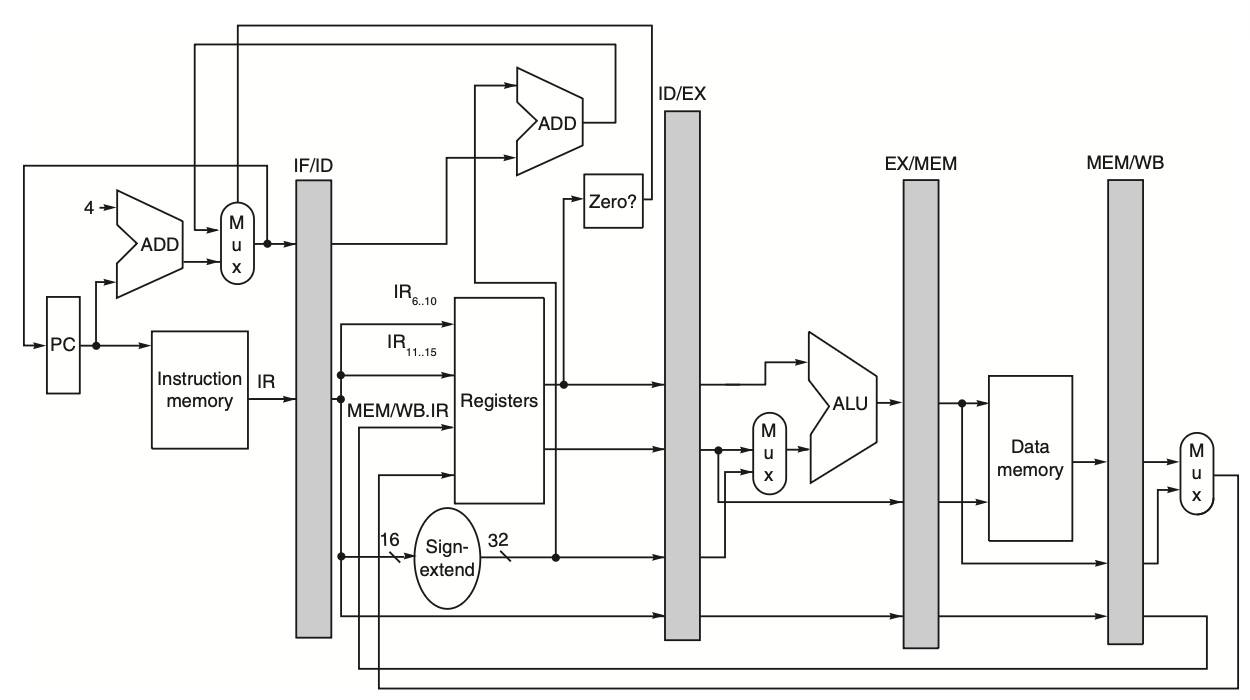
\includegraphics[width=\linewidth]{assets/figures/diag-46.png}
\diagramsource{H\&P Fig.~C.28, \hppage{C}{42} (image supplied by the note-taker; zero test and branch-target adder moved into ID); cf.\ \nolinkurl{03-pipelining-lecture.pdf}, slide 61 (``Pipelined MIPS Datapath'')}
\end{minipage}
\end{center}
{\small \emph{Modified MIPS pipeline: conditional branch completed in the ID
stage; branch penalty $=2-1=1$ cycle.}}

\paragraph{Branch stall impact}

\begin{eg}[Impact of a 3-cycle branch stall]
If CPI $=1$ and $30\%$ of instructions are branches with a 3-cycle stall:
new CPI $= 1 + 0.30\times3 = 1.9$ -- almost double! Reducing the penalty to
1 cycle (MIPS solution above) is therefore very valuable.
\end{eg}

\subsubsection{Four Branch Hazard Alternatives}
\label{sec:branch-alternatives}

\paragraph{\#1: Stall until branch direction is clear}
Simplest, but wastes cycles as shown above.

\paragraph{\#2: Predict Branch Not Taken (most common)}
\begin{itemize}
  \item Execute successor instructions in sequence.
  \item ``Squash'' instructions in the pipeline if the branch is actually
  taken.
  \item Advantage: late pipeline state update (nothing irrevocable has
  happened yet).
  \item About $47\%$ of MIPS branches are not taken on average.
  \item $PC+4$ is already calculated, so it is used to fetch the next
  instruction.
\end{itemize}

\textbf{Predict-not-taken timing (branch penalty $=1$ cycle, ID-stage resolution).}
\begin{lstlisting}[caption={Not taken (no stall)}]
                c1    c2    c3    c4    c5    c6    c7
Untaken branch  IF    ID    EX    MEM   WB
Instr i+1             IF    ID    EX    MEM   WB
Instr i+2                   IF    ID    EX    MEM   WB
\end{lstlisting}
\begin{lstlisting}[caption={Taken (1 idle cycle)}]
                c1    c2    c3    c4    c5    c6    c7
Taken branch    IF    ID    EX    MEM   WB
Instr i+1             IF    idle  idle  idle  idle
Branch target               IF    ID    EX    MEM   WB
\end{lstlisting}
\begin{prop}[Branch stall cycles]
\[
  \text{Pipeline stall cycles from branches} = \text{frequency of taken branches} \times \text{branch penalty}
\]
\end{prop}

\paragraph{\#3: Predict Branch Taken}
\begin{itemize}
  \item About $53\%$ of MIPS branches are taken on average.
  \item But (in the basic MIPS pipeline) the branch target address hasn't
  been calculated yet, so MIPS still incurs a 1-cycle branch penalty even
  with this scheme (other machines that know the branch target before the
  outcome can benefit more).
\end{itemize}

\paragraph{\#4: Delayed Branch}

\begin{definition}[Delayed branch]
Define the branch to take place \emph{after} a following instruction:
\begin{lstlisting}
branch instruction
  sequential successor 1  <- branch delay slot(s)
  ...
  sequential successor n
branch target if taken
\end{lstlisting}
A single delay slot suffices for proper branch-decision and branch-target
computation in a 5-stage pipeline. \textbf{MIPS uses this.}\HPA[25]{C}{\S C.2, Figure~C.14}{23}
\end{definition}

\textbf{Delayed branch timing (no stalls, whether or not taken).}
\begin{lstlisting}
                c1    c2    c3    c4    c5    c6    c7
Untaken branch  IF    ID    EX    MEM   WB
Delay slot i+1        IF    ID    EX    MEM   WB
Instr i+2                   IF    ID    EX    MEM   WB
\end{lstlisting}
\begin{lstlisting}
                c1    c2    c3    c4    c5    c6    c7
Taken branch    IF    ID    EX    MEM   WB
Delay slot i+1        IF    ID    EX    MEM   WB
Branch target               IF    ID    EX    MEM   WB
\end{lstlisting}
The behaviour of the delay-slot instruction is the same whether or not the
branch is taken.

\paragraph{Scheduling branch delay slots}

\begin{center}
\begin{tabular}{@{}p{4.6cm}p{4.6cm}p{4.6cm}@{}}
\toprule
\textbf{A. From before branch} & \textbf{B. From branch target} & \textbf{C. From fall-through} \\
\midrule
\begin{lstlisting}
add $1,$2,$3
if $2=0 then
  (delay slot)
\end{lstlisting}
becomes
\begin{lstlisting}
if $2=0 then
  add $1,$2,$3
\end{lstlisting}
&
\begin{lstlisting}
sub $4,$5,$6
add $1,$2,$3
if $1=0 then
  (delay slot)
\end{lstlisting}
becomes
\begin{lstlisting}
sub $4,$5,$6
add $1,$2,$3
if $1=0 then
  sub $4,$5,$6
\end{lstlisting}
&
\begin{lstlisting}
add $1,$2,$3
if $1=0 then
  (delay slot)
or  $7,$8,$9
sub $4,$5,$6
\end{lstlisting}
becomes
\begin{lstlisting}
add $1,$2,$3
if $1=0 then
  or $7,$8,$9
sub $4,$5,$6
\end{lstlisting}
\\
\bottomrule
\end{tabular}
\end{center}

\begin{itemize}
  \item \textbf{A} is the best choice: it always improves performance
  (fills the delay slot without duplicating any instruction, reducing
  instruction count). The branch must not depend on the rescheduled
  instruction.
  \item In \textbf{B}, the moved instruction may need to be \emph{copied},
  increasing instruction count; it must be safe to execute even if the
  branch is not taken.
  \item In \textbf{C}, the instruction must be safe to execute even if the
  branch \emph{is} taken.
\end{itemize}

\textbf{Three cases for choosing the delay-slot instruction.}
\begin{description}[leftmargin=2.2cm,style=nextline]
  \item[A -- independent instruction from before the branch (\emph{common})]
  Always improves performance when used; the branch must not depend on the
  rescheduled instruction.
  \item[B -- instruction from the branch target] Improves performance if
  the branch is taken; may require duplication; must be safe if the branch
  is \emph{not} taken.
  \item[C -- instruction from the fall-through stream] Improves performance
  if the branch is \emph{not} taken; must be safe if the branch \emph{is}
  taken.
\end{description}
\begin{remark}
The usability of cases B and C is improved by using a \textbf{canceling
(nullifying) branch}.
\end{remark}

\paragraph{Delayed branch: compiler effectiveness}

\begin{itemize}
  \item Fills about $60\%$ of branch delay slots.
  \item About $80\%$ of instructions placed in delay slots are useful.
  \item $\Rightarrow$ about $50\%$ ($60\%\times80\%$) of slots are
  \emph{usefully} filled.
\end{itemize}
\begin{remark}
\textbf{Downside:} as processors move to deeper pipelines and multiple
issue, the branch delay grows and more than one delay slot is needed.
Delayed branching has lost popularity relative to more flexible (but more
expensive) dynamic approaches, since growth in available transistors has
made dynamic branch prediction relatively cheaper.
\end{remark}

\paragraph{Evaluating branch alternatives}

\begin{prop}[Pipeline speedup with branches]
\[
  \text{Pipeline speedup} = \frac{\text{Pipeline depth}}{1+\text{Branch frequency} \times \text{Branch penalty}}
\]\HPA[27]{C}{\S C.2, Performance of Branch Schemes}{25}
\end{prop}

\begin{eg}[Comparing branch schemes]
Assume $4\%$ unconditional branches, $6\%$ untaken conditional branches and
$10\%$ taken conditional branches.

\begin{center}
\small
\begin{tabular}{@{}lcccc@{}}
\toprule
Scheme & Branch penalty & CPI & vs.\ unpipelined & vs.\ stall \\
\midrule
Stall pipeline    & 3                         & 1.60 & 3.1 & 1.00 \\
Predict not taken & $1{\times}0.04+3{\times}0.10$ & 1.34 & 3.7 & 1.19 \\
Predict taken     & $1{\times}0.14+2{\times}0.06$ & 1.26 & 4.0 & 1.29 \\
Delayed branch    & 0.5                       & 1.10 & 4.5 & 1.45 \\
\bottomrule
\end{tabular}
\end{center}

\end{eg}

\paragraph{Pipeline performance example}

\begin{eg}[CPI of a realistic mix]
MIPS instruction mix:

\begin{center}
\begin{tabular}{@{}lp{9.5cm}@{}}
\toprule
Type & Frequency \\
\midrule
Arith/Logic & 40\% \\
Load        & 30\% (of which 25\% are immediately followed by an instruction using the loaded value) \\
Store       & 10\% \\
Branch      & 20\% (of which 45\% are taken) \\
\bottomrule
\end{tabular}
\end{center}

With forwarding and branch-address calculation in the ID stage, using a
branch-not-taken scheme (branch penalty $=1$ cycle):
\[
  \mathrm{CPI} = 1 + \underbrace{0.3\times0.25\times1}_{\text{load-use stalls}} + \underbrace{0.2\times0.45\times1}_{\text{branch stalls}} = 1 + 0.075 + 0.09 = 1.165
\]
\end{eg}

% =============================================================================
\subsection{Textbook Exercises}
\label{sec:pipe-tbx}

\begin{tbexercise}[C]{C.1}{82}{\S C.2, \hppages{C}{11}{27}}
\begin{lstlisting}
Loop: LD    R1,0(R2)    ; load R1 from address 0+R2
      DADDI R1,R1,#1    ; R1 = R1+1
      SD    R1,0(R2)    ; store R1 at address 0+R2
      DADDI R2,R2,#4    ; R2 = R2+4
      DSUB  R4,R3,R2    ; R4 = R3-R2
      BNEZ  R4,Loop     ; branch to Loop if R4 != 0
\end{lstlisting}
Initially R3 $=$ R2 $+$ 396. (a) List all data dependences (register, source,
destination). (b) Draw the timing on the 5-stage pipeline without forwarding (a
register written and read in the same cycle is forwarded through the register file),
branches handled by flushing; how many cycles does the loop take? (c) With full
forwarding, predict not taken. (d) With full forwarding, predict taken. (e) A 10-stage
pipeline splits every stage in two; forwarding goes from the end of a pair of stages
to the start of the pair that needs it; predict taken. (f) The longest 5-stage stage
takes 0.8 ns and the pipeline register 0.1 ns: the cycle time of the 5- and 10-stage
machines? (g) The CPI of the loop on each, and the average instruction time.
\end{tbexercise}

\begin{tbexercise}[C]{C.2}{83}{\S C.2 (branch penalties), \hppages{C}{21}{27}}
Conditional branches are 15\% of instructions (60\% taken), jumps and calls 1\%.
(a) In a 4-deep pipeline, unconditional branches resolve at the end of cycle 2 and
conditional ones at the end of cycle 3; only the first stage is independent of the
branch outcome. How much faster would the machine be without branch hazards? (b) The
same for a 15-deep pipeline resolving at the end of cycles 5 and 10.
\end{tbexercise}

\begin{tbexercise}[C]{C.3}{83}{\S C.1--C.2, \hppages{C}{10}{13}}
A single-cycle machine has a 7 ns clock. Split into stages: IF 1, ID 1.5, EX 1, MEM 2,
WB 1.5 ns; pipeline register delay 0.1 ns. (a) Clock cycle of the 5-stage pipeline?
(b) CPI with a stall every 4 instructions? (c) Speedup over the single-cycle machine?
(d) Speedup with infinitely many stages?
\end{tbexercise}

\begin{tbexercise}[C]{C.4}{84}{\S C.2, \hppages{C}{21}{23}}
Resolving branches in ID instead of MEM reduces control stalls but can create a new
data hazard. Write a short code snippet where computing the branch in ID causes a
data hazard even with forwarding.
\end{tbexercise}


\section{Cache}
\label{sec:cache}
\sources{Lecture ``Memory Hierarchy Design'' (\nolinkurl{04-cache-lecture.pdf});
Group~1 ``Cache'' (\nolinkurl{04-cache-group1.pdf}); H\&P 5th ed.\ App.~B
(\S B.1--B.3) and Ch.~2 (\S2.1--2.2).}

% =============================================================================
\subsection{The Memory Hierarchy}
\label{sec:hierarchy}

\paragraph{The processor--memory gap.} Since 1980 processor performance has
grown about 60\% per year but DRAM latency only about 9\% per year, so the gap
grew about 50\% per year. A four-issue 2~GHz superscalar waiting on a 100~ns DRAM
access could have executed 800 instructions in that time. The goal of the
hierarchy is the \emph{illusion of a memory as large as the cheapest level and as
fast as the fastest}.\HP{\S2.1, Figure~2.2}{74}

\begin{center}
\small
\begin{tabular}{@{}lllll@{}}
\toprule
Level & Typical size & Technology & Access time & Managed by \\
\midrule
Registers & $<1$ KB & custom CMOS & 0.15--0.3 ns & compiler \\
Cache & 32 KB--8 MB & on-chip SRAM & 0.5--15 ns & hardware \\
Main memory & $<512$ GB & DRAM & 30--200 ns & operating system \\
Disk & $>1$ TB & magnetic disk / flash & $\approx5{,}000{,}000$ ns & OS / operator \\
\bottomrule
\end{tabular}
\end{center}
Moving down the hierarchy, each level is larger, slower and cheaper per byte; the
unit moved between levels grows: words (registers), \textbf{blocks} or lines of
8--128 bytes (cache), \textbf{pages} of 4--64 KB (memory).\HPA{B}{\S B.1, Figure~B.1}{3}

\begin{definition}[Locality]
\textbf{Temporal locality}: a location referenced now is likely to be referenced
again soon (loops, reused variables). \textbf{Spatial locality}: locations near
one just referenced are likely to be referenced soon (sequential code, array
traversal). Rule of thumb: a program spends 90\% of its time in 10\% of its
code. Caches exploit temporal locality by \emph{keeping} recently used data and
spatial locality by fetching whole \emph{blocks}.
\end{definition}

\begin{definition}[Basic terms]
A \textbf{block} (line) is the unit copied between two adjacent levels. A
\textbf{hit}: the data is found in the upper level; \textbf{hit time} is the time
to access it, including deciding hit or miss. A \textbf{miss}: the block must be
fetched from the lower level; the \textbf{miss penalty} is the time to replace a
block and deliver the data to the processor. Hit rate $=$ hits/accesses; miss rate
$=1-$ hit rate.\HPA{B}{\S B.1}{2}
\end{definition}

\begin{eg}[Locality in a loop]
\texttt{for (i = 0; i < 10; i++) S = S + A[i];} Without a cache this makes at
least 12 memory accesses (10 reads of \texttt{A[i]}, read and write \texttt{S}). If
\texttt{A[0..9]} and \texttt{S} fit in one 32-byte block, the cache needs one
access to load the block and one to write it back. \texttt{S} shows temporal
locality, \texttt{A[i]} spatial locality.
\end{eg}

% =============================================================================
\subsection{The Four Questions}
\label{sec:four-questions}

Every level of the hierarchy answers four questions:\HPA{B}{\S B.1}{6}
\begin{enumerate}
  \item \textbf{Block placement}: where can a block be placed? (direct mapped,
  set associative, fully associative)
  \item \textbf{Block identification}: how is a block found? (tag, index, valid bit)
  \item \textbf{Block replacement}: which block is replaced on a miss? (random,
  LRU, FIFO and LRU approximations)
  \item \textbf{Write strategy}: what happens on a write? (write-through or
  write-back; write allocate or not)
\end{enumerate}

\subsubsection{Q1: Block placement}
\begin{definition}[Cache organizations]
With $C$ = cache size, $B$ = block size and $a$ = associativity:
\begin{itemize}
  \item \textbf{Direct mapped}: each block has exactly one place,
  (block address) mod (number of blocks).
  \item \textbf{$n$-way set associative}: the cache has $S=C/(B\cdot n)$
  \emph{sets} of $n$ blocks (\emph{ways}); a block goes in set
  (block address) mod $S$, in any of its ways.
  \item \textbf{Fully associative}: a block can go anywhere (one set).
\end{itemize}
Direct mapped is 1-way set associative; fully associative with $m$ blocks is
$m$-way set associative.\HPA{B}{\S B.1, Figure~B.2}{7}
\end{definition}

\begin{center}\begin{minipage}{\linewidth}\centering
\begin{tikzpicture}[font=\scriptsize,x=0.42cm,y=0.42cm]
  \node[font=\small\bfseries] at (4,3.2) {Fully associative};
  \fill[black!15] (0,0) rectangle (8,1);
  \foreach \i in {0,...,7} {\draw (\i,0) rectangle ++(1,1); \node at (\i+0.5,-0.5) {\i};}
  \node at (4,2) {block 12: anywhere};
  \node[font=\small\bfseries] at (15,3.2) {2-way set associative};
  \fill[black!15] (11,0) rectangle (13,1);
  \foreach \i in {11,...,18} {\draw (\i,0) rectangle ++(1,1);}
  \foreach \x in {11,13,15,17,19} {\draw[very thick] (\x,-0.15) -- (\x,1.15);}
  \foreach \s/\x in {0/12,1/14,2/16,3/18} {\node at (\x,-0.5) {set \s};}
  \node at (15,2) {block 12: set $12 \bmod 4 = 0$};
  \node[font=\small\bfseries] at (26,3.2) {Direct mapped};
  \fill[black!15] (26,0) rectangle (27,1);
  \foreach \i/\n in {22/0,23/1,24/2,25/3,26/4,27/5,28/6,29/7} {\draw (\i,0) rectangle ++(1,1); \node at (\i+0.5,-0.5) {\n};}
  \node at (26,2) {block 12: $12 \bmod 8 = 4$};
\end{tikzpicture}
\diagramsource{\nolinkurl{04-cache-lecture.pdf}, handout p.~4, slide 14 (``Q1: Where can a block be placed?''); Group~1 slide 19 (``Q1: Where Can a Block Be Placed in a Cache?''); cf.\ H\&P Fig.~B.2, \hppage{B}{8}}
\end{minipage}
\end{center}
\noindent An 8-block cache and memory block 12: the shaded frames are where it may
go.

\begin{itemize}
  \item \textbf{Direct mapped}: simple and fast, but a high miss rate when two
  busy blocks share an index (the ``ping-pong'' effect): a block is replaced while
  other frames are empty.
  \item \textbf{Fully associative}: needs a comparator per block (content
  addressable memory, CAM); a block is replaced only when the cache is full; costly
  in area, power and delay, so used only for small structures (TLBs).
  \item \textbf{Set associative}: the compromise used in practice (Intel, AMD:
  2- to 16-way); $n$ comparators and an $n$-to-1 multiplexer.
\end{itemize}

\subsubsection{Q2: Block identification}
\begin{center}\begin{minipage}{\linewidth}\centering
\begin{tikzpicture}[font=\small]
  \node[draw,minimum width=4.6cm,minimum height=0.6cm] (t) {Tag};
  \node[draw,minimum width=3cm,minimum height=0.6cm,right=0pt of t] (i) {Index};
  \node[draw,minimum width=2.4cm,minimum height=0.6cm,right=0pt of i] (o) {Block offset};
  \node[font=\scriptsize,below=1pt of t] {$t=A-k-b$ bits};
  \node[font=\scriptsize,below=1pt of i] {$k=\log_2 S$ bits};
  \node[font=\scriptsize,below=1pt of o] {$b=\log_2 B$ bits};
  \draw[decorate,decoration={brace,amplitude=4pt}] (t.north west) -- node[above=4pt,font=\scriptsize]{block address $=\lfloor\text{addr}/B\rfloor$} (i.north east);
\end{tikzpicture}
\diagramsource{\nolinkurl{04-cache-lecture.pdf}, handout p.~7, slide 25 (``Q2: How is a block found?''); Group~1 slide 31; cf.\ H\&P Fig.~B.3, \hppage{B}{9}}
\end{minipage}
\end{center}
\begin{prop}[Address fields]
For an $A$-bit byte address: \textbf{offset} $b=\log_2 B$ bits selects the byte in
the block; \textbf{index} $k=\log_2 S$ bits selects the set; the remaining
$t=A-k-b$ bits are the \textbf{tag}, compared with the tags stored in every way of
the set. A \textbf{valid bit} per block says whether the entry holds data (it is 0
after reset).\HPA{B}{\S B.1, Figure~B.3}{8}
\[
  S=\frac{C}{B\times a},\qquad \text{set}=\text{block address}\bmod S,\qquad
  \text{tag}=\left\lfloor\frac{\text{block address}}{S}\right\rfloor .
\]
\end{prop}
\begin{itemize}
  \item With $C$ and $B$ fixed, doubling the associativity halves the sets: the
  index loses a bit and the tag gains one. Fully associative caches have no index.
  \item Storage per block $=8B$ data bits $+$ tag $+$ valid ($+$ dirty for
  write-back) ($+$ replacement state).
\end{itemize}

\begin{eg}[Three caches from the slides]
All with 32-bit byte addresses.
\begin{center}
\small
\begin{tabular}{@{}lllll@{}}
\toprule
Cache & Blocks & Offset & Index & Tag \\
\midrule
4 KB direct mapped, 1-word blocks & 1024 & 2 & 10 & 20 \\
64 KB direct mapped, 4-word blocks & 4096 & 4 & 12 & 16 \\
4 KB 4-way, 1-word blocks (256 sets) & 1024 & 2 & 8 & 22 \\
\bottomrule
\end{tabular}
\end{center}
The 64 KB cache uses the 2 offset bits above the byte offset to select one of the
4 words (a multiplexer). The 4-way cache compares 4 tags in parallel and selects
the hit way with a 4-to-1 multiplexer, which lengthens the hit time.
\end{eg}

\begin{eg}[Mapping a byte address]
A direct-mapped cache has 64 blocks of 16 bytes. Byte address 1200 is in memory
block $\lfloor1200/16\rfloor=75$ (bytes 1200--1215), which maps to cache block
$75\bmod64=11$. In bits: offset $=$ low 4 bits, index $=$ next 6 bits $=001011_2=11$.
\end{eg}

\subsubsection{Q3: Block replacement}
Direct mapped has no choice. For set-associative and fully associative caches:
\begin{itemize}
  \item \textbf{Random}: spread allocation uniformly; often pseudo-random so
  behaviour is reproducible for debugging. Simplest hardware.
  \item \textbf{Least recently used (LRU)}: replace the block unused for the
  longest time (a corollary of locality). The state must be updated on every
  access; exact LRU needs the full order of the $n$ ways ($\lceil\log_2 n!\rceil$
  bits per set), so it is only feasible for small sets (2- or 4-way).
  \item \textbf{First in, first out (FIFO)}, also round-robin: replace the oldest
  block; hits do not change the order. Used in highly associative caches.
\end{itemize}
Replacement has a \emph{second-order} effect: it acts only on misses. For large
caches LRU, random and FIFO differ by under 1\%; for a 16~KB 2-way cache the
data misses per 1000 instructions are 114.1 (LRU), 117.3 (random), 115.5
(FIFO).\HPA{B}{\S B.1, Figure~B.4}{10}

\paragraph{LRU approximations.}
\begin{itemize}
  \item \textbf{Tree pseudo-LRU} (the lecturer's slides; common for 4--8 ways):
  $n-1$ bits form a binary tree over the ways. For 4 ways, $b_0$ chooses the pair
  ($\{0,1\}$ or $\{2,3\}$), $b_1$ the way in $\{0,1\}$, $b_2$ the way in $\{2,3\}$.
  On every access the bits on the path are set to point \emph{away} from the
  accessed way; the victim is found by following the bits from the root.
  \item \textbf{One bit per way} (the pseudo-LRU of H\&P): an access sets the bit
  of its way; when all bits of a set are 1 they are cleared except the newest; the
  victim is a way whose bit is 0.\HPA[10]{B}{\S B.1}{9}
  \item \textbf{Clock} (second chance): the ways form a circle with one reference
  bit each and a pointer. An access sets the bit. To replace, look at the pointed
  way: if its bit is 1, clear it and advance; replace the first way whose bit is 0.
  The new block gets bit 1 and the pointer moves past it. The same algorithm
  approximates LRU for pages (Section~\ref{sec:vm-replacement}).
\end{itemize}

\begin{center}\begin{minipage}{\linewidth}\centering
\begin{tikzpicture}[font=\small,level distance=1.1cm,
  level 1/.style={sibling distance=3.6cm},level 2/.style={sibling distance=1.6cm}]
  \node[tnode] {$b_0$}
    child {node[tnode] {$b_1$}
      child {node[box] {way 0} edge from parent node[left,font=\scriptsize]{0}}
      child {node[box] {way 1} edge from parent node[right,font=\scriptsize]{1}}
      edge from parent node[left,font=\scriptsize]{0}}
    child {node[tnode] {$b_2$}
      child {node[box] {way 2} edge from parent node[left,font=\scriptsize]{0}}
      child {node[box] {way 3} edge from parent node[right,font=\scriptsize]{1}}
      edge from parent node[right,font=\scriptsize]{1}};
  \node[align=left,font=\scriptsize,anchor=west] at (4.2,-1.2)
    {Access way 0: $b_0\leftarrow1$, $b_1\leftarrow1$\\
     Access way 2: $b_0\leftarrow0$, $b_2\leftarrow1$\\
     Victim: follow $b_0$, then $b_1$ or $b_2$};
\end{tikzpicture}
\diagramsource{own diagram; the lecturer's slide 28 (\nolinkurl{04-cache-lecture.pdf}, handout p.~8) only names ``pseudo-LRU binary tree''; bit convention as defined in the text, traced in the example below}
\end{minipage}
\end{center}

\begin{eg}[Four policies on one 4-way set]
Block references \texttt{0 1 2 3 0 4 1 0 5 2 3 0}, set initially empty (fill ways
0--3 in order; tree bits $b_0b_1b_2$ start at 000; Clock gives new blocks bit 1).
M $=$ miss (victim), H $=$ hit.
\begin{center}
\scriptsize
\setlength{\tabcolsep}{2.4pt}
\begin{tabular}{@{}lcccccccccccc@{}}
\toprule
Ref & 0 & 1 & 2 & 3 & 0 & 4 & 1 & 0 & 5 & 2 & 3 & 0 \\
\midrule
LRU & M & M & M & M & H & M(1) & M(2) & H & M(3) & M(4) & M(1) & H \\
FIFO & M & M & M & M & H & M(0) & H & M(1) & M(2) & M(3) & M(4) & H \\
Tree & M & M & M & M & H & M(2) & H & H & M(3) & M(1) & M(4) & H \\
\quad $b_0b_1b_2$ & 110 & 100 & 001 & 000 & 110 & 011 & 101 & 111 & 010 & 100 & 001 & 111 \\
Clock & M & M & M & M & H & M(0) & H & M(2) & M(3) & M(1) & M(4) & H \\
\bottomrule
\end{tabular}
\end{center}
Misses: LRU 9, FIFO 9, Tree 8, Clock 9. At reference 4 the tree bits are 110
($b_0=1$: right pair; $b_2=0$: way 2), so the tree evicts block 2 while true LRU
evicts block 1: tree PLRU only approximates LRU (here, by luck, it does better).
Clock at reference 4 finds every bit set, clears all four and evicts block 0.
\end{eg}

\subsubsection{Q4: Write strategy}
Reads dominate: with 26\% loads and 10\% stores, writes are about 7\% of all
memory traffic and 28\% of data-cache traffic. A read can access the block while
the tag is checked; a write cannot modify the block until the tag matches, so
writes are slower.\HPA[11]{B}{\S B.1}{10}
\begin{definition}[Write policies]
On a write \textbf{hit}:
\begin{itemize}
  \item \textbf{Write-through}: write both the cache block and the lower level.
  Simple; the lower level always has the current data (simplifies coherence and
  I/O); a read miss never causes a write. Uses a \textbf{write buffer} so the
  processor need not wait (\emph{write stall} otherwise).
  \item \textbf{Write-back}: write only the cache; a modified block is written to
  the lower level when it is replaced. A \textbf{dirty bit} marks modified blocks so
  clean blocks are not written back. Writes run at cache speed, several writes to
  a block cost one write-back, less bandwidth and power.
\end{itemize}
On a write \textbf{miss}:
\begin{itemize}
  \item \textbf{Write allocate} (fetch on write): load the block, then write as on
  a hit.
  \item \textbf{No-write allocate}: write only the lower level; the cache is not
  changed.
\end{itemize}
Usual pairs: write-back $+$ write allocate; write-through $+$ no-write
allocate.\HPA[12]{B}{\S B.1}{11}
\end{definition}

\begin{eg}[Write allocate vs.\ no-write allocate]
A fully associative write-back cache, initially empty, sees
\texttt{Write M[100]; Write M[100]; Read M[200]; Write M[200]; Write M[100]}.
No-write allocate: 100 is never brought in, so both writes to 100 and the last
one miss; the read of 200 misses and loads it; the write to 200 hits: \textbf{4
misses, 1 hit}. Write allocate: only the first accesses to 100 and 200 miss:
\textbf{2 misses, 3 hits}.\HPA{B}{\S B.1, Example}{12}
\end{eg}

\begin{eg}[A real cache: AMD Opteron L1 data cache]
64 KB, 64-byte blocks, 2-way set associative, LRU, write-back, write allocate. So
$64\text{K}/(64\times2)=512$ sets: 9 index bits, 6 offset bits; the 40-bit
physical address leaves a $40-9-6=25$-bit tag. A victim buffer holds blocks being
written back.\HPA[14]{B}{\S B.1, Figure~B.5}{12}
\end{eg}

% =============================================================================
\subsection{Cache Performance}
\label{sec:cache-perf}

\begin{theorem}[CPU time with memory stalls]
\begin{align*}
  \text{CPU time} &= (\text{CPU clock cycles}+\text{Memory stall cycles})\times\text{Clock cycle time}\\
  \text{Memory stall cycles} &= \text{IC}\times\frac{\text{Misses}}{\text{Instruction}}\times\text{Miss penalty}\\
  &= \text{IC}\times\frac{\text{Memory accesses}}{\text{Instruction}}\times\text{Miss rate}\times\text{Miss penalty}
\end{align*}
Every instruction makes one instruction fetch, plus a data access if it is a
load or store. Hit cycles are counted in the CPU clock cycles.\HPA[5]{B}{\S B.1}{4}
\end{theorem}

\begin{eg}[Cost of misses]
$\CPI=1.0$ when all accesses hit; loads and stores are 50\% of instructions; miss
penalty 25 cycles; miss rate 2\%. Stall cycles per instruction
$=(1+0.5)\times0.02\times25=0.75$, so $\CPI=1.75$: the perfect cache would be
$1.75\times$ faster.\HPA{B}{\S B.1, Example}{5}
\end{eg}

\begin{definition}[Average memory access time]
\[
  \AMAT=\text{Hit time}+\text{Miss rate}\times\text{Miss penalty}.
\]
It is a better measure than miss rate, but still not a substitute for execution
time.\HPA{B}{\S B.2}{16} Misses per instruction and miss rate are related by
$\dfrac{\text{Misses}}{\text{Instruction}}=\text{Miss rate}\times\dfrac{\text{Memory accesses}}{\text{Instruction}}$;
data are often given as misses per 1000 instructions (MPKI).
\end{definition}

\begin{eg}[Split or unified cache?]
16 KB I-cache $+$ 16 KB D-cache vs.\ a 32 KB unified cache. Misses per 1000
instructions: 3.82 (16 KB I), 40.9 (16 KB D), 43.3 (32 KB unified); 36\% of
instructions are loads/stores, so 74\% of accesses are instruction fetches
($1/1.36$). Hit 1 cycle, miss penalty 200 cycles; the single-ported unified cache
adds 1 cycle to a data access (structural hazard).
Miss rates: $3.82/1000=0.004$; $40.9/1000/0.36=0.114$;
$43.3/1000/1.36=0.0318$. Split overall $0.74(0.004)+0.26(0.114)=0.0326$.
\begin{align*}
  \AMAT_{split}&=0.74(1+0.004\cdot200)+0.26(1+0.114\cdot200)=7.52\\
  \AMAT_{unified}&=0.74(1+0.0318\cdot200)+0.26(1+1+0.0318\cdot200)=7.62
\end{align*}
The unified cache has the lower miss rate, but the split caches win on AMAT
because they give two ports per cycle.\HPA[17]{B}{\S B.2, Example and Figure~B.6}{15}
\end{eg}
\begin{remark}
\textbf{Textbook typo.} The book states a miss penalty of 100 cycles in this
example but computes with 200; the numbers above follow the book's computation.
\end{remark}

\begin{eg}[In-order processor]
Miss penalty 200 cycles, $\CPI_{exec}=1.0$, miss rate 2\%, 1.5 memory references
per instruction (30 misses per 1000 instructions):
$\CPI=1.0+1.5\times0.02\times200=1.0+30/1000\times200=7.0$. With no cache at all:
$1.0+1.5\times200=301$. The lower the $\CPI_{exec}$ and the faster the clock, the
larger the relative impact of a miss.\HPA[19]{B}{\S B.2, Example}{18}
\end{eg}

% =============================================================================
\subsection{The Three Cs}
\label{sec:three-cs}

\begin{definition}[Miss categories]
\begin{itemize}
  \item \textbf{Compulsory} (cold-start, first-reference): the very first access
  to a block. They occur even in an infinite cache.
  \item \textbf{Capacity}: the cache cannot hold all blocks the program needs, so
  blocks are discarded and later retrieved. They occur in a fully associative
  cache of the same size.
  \item \textbf{Conflict} (collision): in a set-associative or direct-mapped
  cache, too many blocks map to one set. They are the misses of an $n$-way cache
  that would hit in the fully associative cache of the same size.
\end{itemize}
Multiprocessors add a fourth C, \textbf{coherence} misses
(Section~\ref{sec:mp}).\HPA{B}{\S B.3}{23}
\end{definition}

\begin{itemize}
  \item In SPEC2000 the compulsory miss rate is tiny (0.0001); for a 4 KB cache the
  total miss rate is 0.098 direct mapped, 0.076 2-way, 0.071 4- or 8-way, and the
  capacity part alone is 0.070.\HPA{B}{\S B.3, Figure~B.8}{24}
  \item \textbf{8-way is as good as fully associative} for these sizes, and the
  \textbf{2:1 cache rule of thumb}: a direct-mapped cache of size $N$ has about the
  miss rate of a 2-way cache of size $N/2$.\HPA{B}{\S B.3}{29}
  \item The model has limits: it ignores replacement, and a miss can change
  category when the cache size changes.\HPA{B}{\S B.3}{26}
\end{itemize}

\begin{eg}[Classifying misses]
A direct-mapped cache of 4 one-word blocks (index $=$ address mod 4), initially
empty; word addresses \texttt{0 4 0 1 2 3 5 0 4 1}:
\begin{center}
\small
\begin{tabular}{@{}lcccccccccc@{}}
\toprule
Address & 0 & 4 & 0 & 1 & 2 & 3 & 5 & 0 & 4 & 1 \\
Index & 0 & 0 & 0 & 1 & 2 & 3 & 1 & 0 & 0 & 1 \\
Result & comp. & comp. & confl. & comp. & comp. & comp. & comp. & hit & cap. & cap. \\
\bottomrule
\end{tabular}
\end{center}
The third access misses only because 4 took index 0 (a 4-block fully associative
LRU cache would still hold 0): conflict. The last two also miss in the fully
associative cache (too many distinct blocks since their last use): capacity.
\end{eg}

% =============================================================================
\subsection{Six Basic Cache Optimizations}
\label{sec:basic-opt}

$\AMAT=\text{Hit time}+\text{Miss rate}\times\text{Miss penalty}$ gives three
targets.\HPA{B}{\S B.3}{22}
\begin{center}
\small
\begin{tabular}{@{}P{4.3cm}P{3.6cm}P{6cm}@{}}
\toprule
Optimization & Improves & Drawback \\
\midrule
1. Larger block size & miss rate (compulsory) & larger miss penalty; fewer blocks, so more conflict (and capacity) misses in small caches \\
2. Larger cache & miss rate (capacity) & longer hit time, cost, power \\
3. Higher associativity & miss rate (conflict) & longer hit time \\
4. Multilevel caches & miss penalty & more hardware; harder analysis \\
5. Read misses before writes & miss penalty & write buffer must be checked \\
6. Avoid address translation when indexing & hit time & needs virtually indexed caches \\
\bottomrule
\end{tabular}
\end{center}

\paragraph{1. Larger blocks.} Exploit spatial locality. The best block size
minimizes AMAT, not the miss rate: in the book's data 32 bytes is best for a 4 KB
cache and 64 bytes for larger ones. High latency and high bandwidth below favour
large blocks.\HPA[28]{B}{\S B.3, Figure~B.12}{26}

\paragraph{2--3. Larger caches, higher associativity.} The obvious cure for capacity
misses; associativity removes conflict misses, but each step can stretch the clock.
\begin{eg}[Associativity vs.\ hit time]
The clock cycle grows by $1.36\times$ (2-way), $1.44\times$ (4-way) and
$1.52\times$ (8-way) over direct mapped; hit 1 cycle, miss penalty 25 cycles. AMAT for a 4 KB direct
mapped cache: $1.00+0.098\times25=3.44$; 512 KB 8-way: $1.52+0.006\times25=1.66$.
Higher associativity pays off only up to about 8 KB; from 16 KB on, the longer
hit time outweighs the saved misses.\HPA[30]{B}{\S B.3, Example}{29}
\end{eg}

\paragraph{4. Multilevel caches.} L1 is small and fast enough to match the
processor clock; L2 is large enough to catch many accesses that would go to
memory, so it reduces the L1 miss penalty.\HPA{B}{\S B.3}{30}
\begin{theorem}[Two-level AMAT]
\[
  \AMAT=\text{Hit time}_{L1}+\text{Miss rate}_{L1}\times
  \big(\text{Hit time}_{L2}+\text{Miss rate}_{L2}\times\text{Miss penalty}_{L2}\big)
\]
\begin{itemize}
  \item \textbf{Local miss rate}: misses in a cache $/$ accesses \emph{to that
  cache} (for L2, the L1 misses). Large for L2, since L1 ``skims the cream''.
  \item \textbf{Global miss rate}: misses in a cache $/$ all memory accesses of the
  processor; for L2 it is $\text{Miss rate}_{L1}\times\text{Miss rate}_{L2}$. The
  better measure for L2.
  \item Stalls per instruction $=\dfrac{\text{Misses}_{L1}}{\text{Instr}}\times\text{Hit time}_{L2}
  +\dfrac{\text{Misses}_{L2}}{\text{Instr}}\times\text{Miss penalty}_{L2}$.
\end{itemize}
\HPA[32]{B}{\S B.3}{31}
\end{theorem}

\begin{eg}[Local and global miss rates]
1000 memory references: 40 L1 misses, 20 L2 misses; L1 hit 1 cycle, L2 hit 10
cycles, memory 200 cycles; 1.5 references per instruction. L1 miss rate $=4\%$;
L2 local $=20/40=50\%$, global $=20/1000=2\%$.
$\AMAT=1+0.04\times(10+0.5\times200)=5.4$ cycles. Per 1000 instructions there are
60 L1 and 30 L2 misses, so stalls per instruction
$=0.060\times10+0.030\times200=6.6$ cycles $=(5.4-1)\times1.5$.\HPA[32]{B}{\S B.3, Example}{31}
\end{eg}

\begin{eg}[Adding an L2 (Group 1)]
L1: hit 1 ns, miss rate 10\%, memory 100 ns. Only L1: $\AMAT=1+0.1\times100=11$ ns.
Add L2: hit 8 ns, local miss rate 20\%, penalty 105 ns:
$\AMAT=1+0.1\times(8+0.2\times105)=3.9$ ns.
\end{eg}

\begin{itemize}
  \item \textbf{Multilevel inclusion}: L1 data are always in L2 (coherence can be
  checked in L2 only). \textbf{Exclusion}: L1 data are never in L2; a miss swaps
  blocks, so a small L2 is not wasted on copies (AMD Opteron).\HPA[35]{B}{\S B.3}{34}
  \item The L1 speed affects the clock; the L2 speed affects only the L1 miss
  penalty. So L2 can be larger, more associative, with larger blocks.
\end{itemize}

\paragraph{5. Read misses before writes.} A read miss is urgent (the processor
waits); a buffered write is not. Let the read go first, but a write buffer may hold
the newest value of the address being read (a read-after-write hazard through
memory): either wait until the buffer drains or, as almost all processors do,
\textbf{check the write buffer} on a read miss. For write-back, copy a dirty victim
to a buffer, read the new block first, then write the victim.\HPA[36]{B}{\S B.3}{35}
\begin{eg}[RAW through the write buffer]
The sequence \texttt{SW R3,512(R0)}; \texttt{LW R1,1024(R0)};
\texttt{LW R2,512(R0)}, where 512 and 1024 map to the same block of a direct-mapped write-through cache. If the
write of 512 is still in the buffer when the second load misses, memory returns
the old value: $R2\ne R3$ unless the buffer is checked.
\end{eg}

\paragraph{6. Avoiding address translation.} A \emph{virtual} cache uses virtual
addresses, removing translation from the hit time, but needs protection checks and
a flush (or a process-ID tag) on a process switch, and can have aliases. The common
solution is a \textbf{virtually indexed, physically tagged} cache: index with page
offset bits while the TLB translates in parallel, then compare physical tags. This
limits $C/a\le$ page size (Section~\ref{sec:vm-cache}).\HPA[40]{B}{\S B.3}{36}

% =============================================================================
\subsection{Advanced Optimizations}
\label{sec:advanced-opt}
\beyond{} Group~1 presented the first and fifth of the ten advanced optimizations
of H\&P Ch.~2; the others are listed for completeness.\HP[96]{\S2.2, Figure~2.11}{78}
\begin{center}
\small
\begin{tabular}{@{}P{5.2cm}P{8.6cm}@{}}
\toprule
Optimization & Idea \\
\midrule
Small and simple L1 & low associativity, small size: short hit time, low power \\
Way prediction & predict the way to read next, like a direct-mapped hit time \\
Pipelined cache access & more cycles per hit but higher bandwidth (and clock) \\
Nonblocking caches & hit under miss, miss under miss: overlap misses \\
Multibanked caches & independent banks serve accesses in parallel \\
Critical word first, early restart & send the requested word before the rest of the block \\
Merging write buffer & combine writes to the same block in one buffer entry \\
Compiler optimizations & loop interchange, blocking: better locality \\
Hardware prefetching & fetch the next block(s) before they are requested \\
Compiler-controlled prefetching & prefetch instructions inserted by the compiler \\
\bottomrule
\end{tabular}
\end{center}

\begin{eg}[Small and simple L1]
Is a 32 KB 4-way L1 faster than a 32 KB 2-way one? Miss rates 3.7\% and 3.8\%;
the 4-way access time is $1.4\times$ the 2-way time; miss penalty $=15\times$ the
2-way access time. In units of the 2-way access time:
$\AMAT_{2}=1+0.038\times15=1.57$, $\AMAT_{4}=1.4+0.037\times15=1.96$. The 2-way
cache wins.\HP{\S2.2, Example}{80}
\end{eg}
\begin{remark}
\textbf{Textbook error.} The book prints $\AMAT_2=1.38$ (an arithmetic slip) and
computes $\AMAT_4=1.4+0.037\times10=1.77$, mixing the 2-way time unit (hit) with
4-way clock cycles (penalty $15/1.4\approx10$). The conclusion is unchanged.
Group~1's slide gives the consistent values 1.57 and 1.96.
\end{remark}

\begin{eg}[Multibanked cache (Group 1)]
4 banks, sequential interleaving (bank $=$ block mod 4), 64-byte blocks; 4 loads per
cycle. Addresses 0, 64, 128, 192 are blocks 0--3 in banks 0--3: 1 cycle. Addresses
0, 256, 512, 192 are blocks 0, 4, 8, 3, three in bank 0: 3 cycles, a bandwidth of
$4/3$ accesses per cycle instead of 4.
\end{eg}

% =============================================================================
\subsection{Worked Problems}
\label{sec:cache-problems}

\begin{eg}[Reading a cache's shape from its address (Group 1)]
A direct-mapped cache uses tag bits 31--10, index 9--5, offset 4--0. Blocks are
$2^5=32$ bytes $=8$ words; there are $2^5=32$ entries. Per entry: 256 data $+$ 22
tag $+$ 1 valid $=279$ bits, a ratio of $279/256\approx1.09$. The byte addresses
0, 4, 16, 132, 232, 160, 1024, 30, 140, 3100, 180, 2180 give
\begin{center}
\small
\setlength{\tabcolsep}{3pt}
\begin{tabular}{@{}lcccccccccccc@{}}
\toprule
Address & 0 & 4 & 16 & 132 & 232 & 160 & 1024 & 30 & 140 & 3100 & 180 & 2180 \\
Index & 0 & 0 & 0 & 4 & 7 & 5 & 0 & 0 & 4 & 0 & 5 & 4 \\
Tag & 0 & 0 & 0 & 0 & 0 & 0 & 1 & 0 & 0 & 3 & 0 & 2 \\
Result & M & H & H & M & M & M & M & M & H & M & H & M \\
\bottomrule
\end{tabular}
\end{center}
4 hits of 12 (33\%), 4 replacements (at 1024, 30, 3100, 2180). Final valid
entries: index 0 tag 3, index 4 tag 2, index 5 tag 0, index 7 tag 0.
\end{eg}

\begin{eg}[Is locality really needed? (H\&P B.1, Group~1)]
Hit 1 cycle, miss 105 cycles (total latency), memory without cache 100 cycles.
(a) Miss rate 5\%: $\AMAT=0.95\times1+0.05\times105=6.2$ cycles ($6.25$ if 105 is
read as an extra penalty after the hit time). (b) Random accesses to a 256 MB
array with a 64 KB cache: a hit has probability $64\text{K}/256\text{M}=1/4096$, so
$\AMAT\approx105$ cycles. (c) That is worse than the 100 cycles without a cache:
\textbf{without locality a cache only hurts}.
\end{eg}

\begin{eg}[Which L1 should we choose? (Group 1)]
Two 32 KB L1 options: A 2-way, hit 0.6 ns, miss rate 5\%; B 8-way, hit 0.8 ns, miss
rate 4\%. L2: 2.8 ns, local miss rate 40\%; L3: 10 ns, 25\%; DRAM 100 ns.
With L3: L1 miss penalty $=2.8+0.4\times(10+0.25\times100)=16.8$ ns;
$\AMAT_A=0.6+0.05\times16.8=1.44$, $\AMAT_B=0.8+0.04\times16.8=1.47$: A wins.
Without L3: penalty $=2.8+0.4\times100=42.8$ ns; $\AMAT_A=2.74$, $\AMAT_B=2.51$: B
wins. B costs 0.2 ns per access and saves 1\% of misses, so it is better only when
the L1 miss penalty exceeds $0.2/0.01=20$ ns.
\end{eg}

% =============================================================================
\subsection{Textbook Exercises}
\label{sec:cache-tbx}

\begin{tbexercise}[B]{B.1}{60}{\S B.1--B.2, \hppages{B}{2}{16}; worked in
Section~\ref{sec:cache-problems}}
Latencies: cache hit 1 cycle, cache miss 105 cycles, main memory with the cache
disabled 100 cycles. (a) Find the AMAT for a 5\% miss rate. (b) A program makes
uniformly random accesses to a 256 MB array; the data cache is 64 KB. Find the AMAT.
(c) Compare with the cache disabled: what does this say about locality? (d) With
gain $G$ per hit and loss $L$ per miss, find the highest miss rate at which the
cache still helps.
\end{tbexercise}

\begin{tbexercise}[B]{B.2}{60}{\S B.1 Q1, \hppage{B}{7}}
A 512-byte cache with 64-byte blocks; main memory of 2 KB $=$ blocks
$M_0,\dots,M_{31}$. For each cache block, list the memory blocks that can reside
in it if the cache is (a) direct mapped; (b) four-way set associative. (Fully
associative: every block can go in each of the 8 cache blocks.)
\end{tbexercise}

\begin{tbexercise}[B]{B.4}{62}{\S B.1 Q4, \hppages{B}{10}{12}}
A 64 KB write-allocate cache with 32-byte lines is connected to memory by an
8-byte bus; a $B$-byte write takes $10+5(\lceil B/8\rceil-1)$ cycles. The loop
writes \texttt{data[j] = j} for \texttt{PORTION} consecutive words starting at
\texttt{8*i}. (a) Write-through: cycles spent on writes for all the \texttt{j}
iterations (\texttt{PORTION} $=1$). (b) Write-back: cycles to write back one line.
(c) Repeat (a) with \texttt{PORTION} $=8$. (d) Minimum number of updates to the same
line before replacement that makes write-back better. (e) Give a case where all
words of a line are written and write-through still needs fewer cycles.
\end{tbexercise}

\begin{tbexercise}[B]{B.5}{62}{\S B.2--B.3, \hppages{B}{16}{35}}
An in-order 1.1 GHz processor has $\CPI=0.7$ without memory stalls; loads are 20\%
and stores 5\% of instructions. Split L1 (no hit penalty): 32 KB direct-mapped
I-cache, 2\% miss rate, 32-byte blocks; 32 KB direct-mapped write-through D-cache,
5\% miss rate, 16-byte blocks, with a write buffer that removes stalls for 95\% of
writes. Unified 512 KB write-back L2, 64-byte blocks, 15 ns access, 128-bit bus at
266 MHz; 80\% of L2 references hit; 50\% of replaced blocks are dirty. Memory:
128 bits wide, 60 ns latency, then one 128-bit word per cycle at 133 MHz. Find the
AMAT of (a) instruction accesses, (b) data reads, (c) data writes, and (d) the
overall CPI.
\end{tbexercise}

\begin{tbexercise}[B]{B.8}{63}{\S B.1 Q3, \hppages{B}{9}{10}; \S B.3}
A fully associative 128-byte instruction cache with 4-byte blocks uses LRU. (a) Find
the asymptotic miss rate of a 64-byte loop executed many times. (b) Repeat for
192- and 320-byte loops. (c) With most-recently-used (MRU) replacement, which of
the three loops benefits? (d) Suggest policies that might beat LRU.
\end{tbexercise}

\begin{tbexercise}[B]{B.9}{64}{\S B.3, \hppages{B}{23}{29}}
Construct a trace of word accesses (one-word blocks) that produces \emph{more}
misses in a 2-way set-associative LRU cache than in a direct-mapped cache of the
same size. (Hint: use addresses that all fall in one set of the 2-way cache but
in two different blocks of the direct-mapped cache.)
\end{tbexercise}

\begin{tbexercise}[B]{B.10}{64}{\S B.3, \hppages{B}{34}{35}}
L1 and L2 data caches are both write-back with the same block size. List the
actions on an L1 miss when the hierarchy is (a) inclusive; (b) exclusive. (c) In
both cases, consider an evicted line that is clean or dirty.
\end{tbexercise}

\begin{tbexercise}{2.11}{138}{\S2.2 (critical word first), \hppages{}{86}{87}}
A 1 MB L2 cache has 64-byte blocks and a 16-byte refill path. The L2 can be
written with 16 bytes every 4 processor cycles; the first 16 bytes arrive from the
memory controller after 120 cycles, each further 16 bytes after 16 more cycles, and
data can be bypassed into the L2 read port. (a) How many cycles does an L2 miss
take with and without critical word first and early restart? (b) Do these
techniques matter more for L1 or for L2 caches, and why?
\end{tbexercise}

\begin{tbexercise}{2.12}{138}{\S2.2 (merging write buffer), \hppages{}{87}{88}}
A write buffer sits between a write-through L1 and a write-back L2. The L2 write
data bus is 16 bytes wide and can write an independent address every 4 processor
cycles. (a) How many bytes wide should each buffer entry be? (b) What steady-state
speedup does a merging buffer give over a nonmerging one when memory is zeroed with
64-bit stores (other instructions issue in parallel, blocks present in L2)? (c) How
do L1 misses affect the number of entries needed with blocking and nonblocking
caches?
\end{tbexercise}

\section{Virtual Memory}
\label{sec:vm}
\sources{Lecture ``Virtual Memory'' (\nolinkurl{05-virtual-memory-lecture.pdf});
Group~2 ``Virtual Memory'' (\nolinkurl{05-virtual-memory-group2.pdf}); H\&P 5th
ed.\ App.~B (\S B.4--B.5) and \S2.4.}

% =============================================================================
\subsection{Why Virtual Memory}
\label{sec:vm-why}

Computers run many processes at once, each wanting a full address space, but
they must share a smaller physical memory. Without virtual memory, programmers
split large programs into \emph{overlays} by hand, programs could overwrite each
other or the OS, free memory became scattered (fragmentation), and whole programs
were loaded up front.\HPA[42]{B}{\S B.4}{40}

\begin{definition}[Virtual memory]
\textbf{Virtual memory} (VM) lets main memory act as a cache for secondary
storage. The processor issues \textbf{virtual} (logical) addresses; hardware (the
MMU) and the OS translate them to \textbf{physical} addresses in main memory or
on disk (\emph{memory mapping}, \emph{address translation}). Each process sees a
large, private address space.
\end{definition}

\paragraph{Benefits.}
\begin{itemize}
  \item \textbf{Larger space}: a program may be larger than physical memory; cold
  pages live on disk (demand paging loads a page on its first access).
  \item \textbf{Isolation and protection}: one page table per process, so the same
  virtual address in two programs maps to different physical frames.
  \item \textbf{Relocation}: a program runs anywhere in physical memory by changing
  the mapping only.
  \item \textbf{Sharing}: several page tables can map the same frame (shared code,
  libraries).
  \item \textbf{Non-contiguous placement}: consecutive virtual pages (e.g.\
  \texttt{A[n]} and \texttt{A[n+1]} across a page boundary) need not be adjacent in
  physical memory.
\end{itemize}
\textbf{Costs}: page tables use memory, translation adds latency (hidden by the
TLB), page faults stall for millions of cycles, and the MMU and TLB cost hardware.

\begin{remark}
\slidefix{} Group~2 lists page-fault stalls as ``disk reads are 1000$\times$
slower''. With a 100~ns memory and a 5--10~ms disk the ratio is about $10^5$, as
their own AMAT example (10~ms vs.\ 100~ns) shows.
\end{remark}

\begin{center}\begin{minipage}{\linewidth}\centering
\begin{tikzpicture}[font=\small,x=1cm,y=0.55cm]
  \node[font=\small\bfseries] at (0.6,4.6) {Virtual};
  \foreach \l/\y/\a in {A/3/0,B/2/4K,C/1/8K,D/0/12K} {
    \draw (0,\y) rectangle ++(1.2,1) node[midway] {\l};
    \node[anchor=east,font=\scriptsize] at (-0.1,\y+0.5) {\a};}
  \node[font=\small\bfseries] at (4.6,4.6) {Physical};
  \foreach \y/\a/\l in {3/0/,2/4K/C,1/8K/,0/12K/,-1/16K/A,-2/20K/,-3/24K/B,-4/28K/} {
    \draw (4,\y) rectangle ++(1.2,1) node[midway] {\l};
    \node[anchor=west,font=\scriptsize] at (5.3,\y+0.5) {\a};}
  \draw[fill=black!10] (7,0) rectangle ++(1.4,1) node[midway] {D};
  \node[font=\small\bfseries] at (7.7,4.6) {Disk};
  \draw[-{Latex}] (1.2,3.5) -- (4,-0.5);
  \draw[-{Latex}] (1.2,2.5) -- (4,-2.5);
  \draw[-{Latex}] (1.2,1.5) -- (4,2.5);
  \draw[-{Latex},dashed] (0.6,0) -- (0.6,-5) -- (7.7,-5) -- (7.7,0);
  \node[font=\scriptsize\itshape,fill=white,inner sep=1pt] at (2.6,-5) {page on disk};
\end{tikzpicture}
\diagramsource{\nolinkurl{05-virtual-memory-lecture.pdf}, handout p.~3 (``Example of virtual memory''); cf.\ H\&P Fig.~B.19, \hppage{B}{41}}
\end{minipage}
\end{center}
\noindent A program of four 4 KB pages: A, B, C are in memory (anywhere), D is on
disk.\HPA{B}{\S B.4, Figure~B.19}{41}


% =============================================================================
\subsection{Paging Vocabulary}
\label{sec:vm-terms}

\begin{definition}[Pages and frames]
A \textbf{(virtual) page} is a fixed-size block of virtual memory; a
\textbf{(physical) frame} is a block of physical memory of the same size (typically
4 KiB; 512 bytes to 16 MB). Any page fits in any frame. The \textbf{page table}
(one per process, indexed by the virtual page number) maps pages to frames; each
\textbf{page table entry} (PTE) holds the frame number and control bits.
\end{definition}

\begin{center}
\small
\begin{tabular}{@{}lP{10.6cm}@{}}
\toprule
Term & Meaning \\
\midrule
VPN & virtual page number: the upper bits of the virtual address \\
PFN / PPN & physical frame (page) number \\
PTE & page table entry: PFN, valid (present), protection (R/W/X, user/supervisor), dirty, reference bits \\
MMU & memory management unit: hardware that translates every access and checks permissions \\
TLB & translation lookaside buffer: a cache of recent translations \\
ASID & address space identifier: tags TLB entries per process, avoiding flushes on a context switch \\
\bottomrule
\end{tabular}
\end{center}

\begin{center}
\small
\begin{tabular}{@{}lll@{}}
\toprule
Cache term & VM term & \\
\midrule
block (line) & page or segment & unit of transfer \\
cache miss & page fault (address fault) & data not in the upper level \\
hit time 1--2 cycles & 40--100 cycles & \\
miss penalty 8--100 cycles & 700{,}000--6{,}000{,}000 cycles & \\
miss rate 0.5--10\% & 0.00001--0.001\% & \\
block 12--128 bytes & page 4096--65{,}536 bytes & \\
size 0.016--1 MB & 4 MB--4 GB & \\
\bottomrule
\end{tabular}
\end{center}
Everything except the miss rate is much worse for VM. Further differences:
cache replacement is done by hardware, page replacement by the OS (so it can
afford to be smart); the processor address size sets the VM size, while the cache
size is independent of it; disk also holds the file system.\HPA[43]{B}{\S B.4, Figure~B.20}{42}

\begin{definition}[Fragmentation]
\textbf{Internal}: fixed-size allocation wastes the unused end of the last page
(on average half a page per region; about 1.5 pages per process with text, heap
and stack). \textbf{External}: variable-size allocation leaves free memory split
into holes too small to use, although their total is large enough. Paging has
only internal fragmentation; segmentation has external
fragmentation.\HPA{B}{\S B.4}{47}
\end{definition}

% =============================================================================
\subsection{Address Translation and Page Tables}
\label{sec:vm-translation}

\begin{center}\begin{minipage}{\linewidth}\centering
\begin{tikzpicture}[font=\small]
  \node[draw,minimum width=4.4cm,minimum height=0.6cm] (vpn) {Virtual page number};
  \node[draw,minimum width=3cm,minimum height=0.6cm,right=0pt of vpn] (off) {Page offset};
  \node[draw,minimum width=2.6cm,minimum height=1.6cm,below=0.9cm of vpn,align=center] (pt) {Page table\\(V, prot., D, R,\\PFN)};
  \node[draw,minimum width=4.4cm,minimum height=0.6cm,below=0.9cm of pt] (pfn) {Physical page number};
  \node[draw,minimum width=3cm,minimum height=0.6cm,right=0pt of pfn] (off2) {Page offset};
  \node[left=0.6cm of pt,align=center,font=\scriptsize] (ptbr) {page-table\\base register};
  \draw[-{Latex}] (vpn) -- node[right,font=\scriptsize]{index} (pt);
  \draw[-{Latex}] (ptbr) -- (pt);
  \draw[-{Latex}] (pt) -- (pfn);
  \draw[-{Latex}] (off.south) -- (off2.north);
  \node[right=2pt of off,font=\scriptsize] {$\log_2$ page size bits};
\end{tikzpicture}
\diagramsource{\nolinkurl{05-virtual-memory-lecture.pdf}, handout p.~2 (``VM: Address Translation''); Group~2 slide 13 (``Page Mapping Translation Flow''); cf.\ H\&P Fig.~B.23, \hppage{B}{45}}
\end{minipage}
\end{center}

\begin{prop}[Translation]
With page size $P$:
\[
  \text{VPN}=\left\lfloor\frac{\text{VA}}{P}\right\rfloor,\qquad
  \text{offset}=\text{VA}\bmod P,\qquad
  \text{PA}=\text{PFN}\times P+\text{offset}.
\]
The offset is not translated; only the page number changes. For paging the offset
is \emph{concatenated} to the frame number; for segmentation it is
\emph{added} to the segment base.\HPA{B}{\S B.4, Figure~B.23}{44}
\end{prop}

\begin{eg}[Hex and decimal translation (Group 2)]
32-bit VA, 4 KiB pages (12-bit offset $=$ the last 3 hex digits). VA
\texttt{0x00403A7C}: VPN \texttt{0x00403}, offset \texttt{0xA7C}; the PTE gives PFN
\texttt{0x1F2}, so PA $=$ \texttt{0x1F2A7C}.

Page size 1024: VA 3500 has VPN $\lfloor3500/1024\rfloor=3$ and offset
$3500-3072=428$; page 3 maps to frame 7, so PA $=7\times1024+428=7596$.
\end{eg}

\begin{prop}[Page table size]
A flat table has one PTE per virtual page:
size $=2^{\text{VA bits}-\log_2P}\times$ PTE size, per process. For a 32-bit VA,
4 KB pages and 4-byte PTEs: $2^{20}\times4=4$ MB per process (400 MB for 100
processes), mostly mapping nothing.\HPA{B}{\S B.4}{44}
\end{prop}
\begin{itemize}
  \item \textbf{Multilevel page tables}: split the VPN; allocate second-level
  tables only for used regions. 32-bit: $10+10+12$ (each level fits in a 4 KB page
  of 1024 four-byte PTEs); x86-64: $9+9+9+9+12$ (48-bit VA, 256 TiB); a TLB miss
  costs one memory access per level.
  \item \textbf{Inverted page table}: one entry per physical frame, found by hashing
  the VPN; its size follows physical memory. A 512 MB memory with 4 KB pages needs
  only 1 MB (8 bytes per entry, including the virtual address) instead of 4 MB per
  process.\HPA[45]{B}{\S B.4}{44}
  \item On x86 the register CR3 holds the root of the active page table and is
  switched on every context switch.
\end{itemize}

% =============================================================================
\subsection{Page Faults}
\label{sec:vm-faults}

\begin{definition}[Page fault]
A \textbf{page fault} is the exception raised when the PTE of an accessed page is
not valid (the page is not in memory). It is the VM analogue of a cache miss, but
handled in \emph{software}: the processor switches to another task during the
disk access.\HPA{B}{\S B.1}{3}
\end{definition}
\begin{enumerate}
  \item The MMU finds a missing or invalid mapping and traps to the OS.
  \item The OS checks the access is legal; an illegal one is rejected (``segmentation
  fault'').
  \item It takes a free frame or chooses a victim; a \textbf{dirty} victim is written
  back first.
  \item It reads the page from disk (or zero-fills a new page).
  \item It updates the PTE and restarts the faulting instruction.
\end{enumerate}
Pinned pages (the fault handler, DMA buffers) never page out. \textbf{Thrashing}:
the working sets of the running processes exceed memory, so the system spends
more time paging than executing; add memory or run fewer processes.

\begin{prop}[Memory access time with page faults]
With hit rate $h$, memory time $T_{mem}$ and disk (fault) time $T_{disk}$, the
lecturer's slide writes $\AMAT=T_{mem}+(1-h)\,T_{disk}$; Group~2 writes
$h\,T_{mem}+(1-h)\,T_{disk}$. They differ by $(1-h)\,T_{mem}$, negligible because
$1-h$ is tiny.
\end{prop}
\begin{eg}[How bad is 99.9\%?]
$T_{mem}=100$ ns, $T_{disk}=10$ ms $=10^7$ ns, $h=99.9\%$:
$0.999\times100+0.001\times10^7\approx10{,}100$ ns, about $101\times$ slower than
memory. With the lecturer's numbers ($T_{disk}=25$ ms) it is $25{,}100$ ns. The
hit rate must be almost perfect.
\end{eg}

% =============================================================================
\subsection{The Four Questions for Virtual Memory}
\label{sec:vm-questions}

\begin{itemize}
  \item \textbf{Q1 Placement}: anywhere in main memory (\textbf{fully associative}):
  the huge miss penalty makes a lower miss rate worth a complex placement.
  \item \textbf{Q2 Identification}: the page table indexed by the VPN (or an inverted
  table), sped up by the TLB.
  \item \textbf{Q3 Replacement}: approximately \textbf{LRU}, by the OS. Hardware
  provides a \emph{use} (reference) bit, set on access; the OS clears the bits
  periodically to see which pages were used recently.
  \item \textbf{Q4 Writes}: always \textbf{write-back} with a dirty bit; nobody
  writes through to disk on every store.
\end{itemize}
\HPA[46]{B}{\S B.4}{44}

\subsubsection{Page replacement algorithms}
\label{sec:vm-replacement}
\begin{center}
\small
\begin{tabular}{@{}lP{5.4cm}P{6.2cm}@{}}
\toprule
Policy & Evicts & Notes \\
\midrule
OPT (optimal) & the page next used furthest in the future & needs the future: a benchmark only \\
FIFO & the page loaded earliest & simple; may evict a busy page; Belady's anomaly \\
LRU & the page unused for the longest time & uses temporal locality; exact tracking is costly \\
LFU & the least frequently used page & keeps once-popular stale pages \\
Clock & first page with reference bit 0 (clearing 1s on the way) & cheap LRU approximation \\
\bottomrule
\end{tabular}
\end{center}

\begin{eg}[FIFO vs.\ LRU (Group 2)]
References \texttt{7 0 1 2 0 3 0 4}, 3 frames. FIFO: 7, 0, 1 fault; 2 evicts 7; 0
hits; 3 evicts 0 (though just used); 0 evicts 1; 4 evicts 2: \textbf{7 faults}. LRU:
2 evicts 7; 0 hits; 3 evicts 1; 0 hits; 4 evicts 2: \textbf{6 faults}.
\end{eg}

\begin{eg}[A string where FIFO beats LRU (lecturer's review)]
3 frames, \texttt{1 2 1 1 3 2 1 4 3 1 1 2 4 1 5 6 2 1}; F $=$ fault (victim).
\begin{center}
\scriptsize
\setlength{\tabcolsep}{2.2pt}
\begin{tabular}{@{}l*{18}{c}@{}}
\toprule
Ref & 1 & 2 & 1 & 1 & 3 & 2 & 1 & 4 & 3 & 1 & 1 & 2 & 4 & 1 & 5 & 6 & 2 & 1 \\
\midrule
FIFO & F & F & & & F & & & F(1) & & F(2) & & F(3) & & & F(4) & F(1) & & F(2) \\
LRU & F & F & & & F & & & F(3) & F(2) & & & F(4) & F(3) & & F(2) & F(4) & F(1) & F(5) \\
OPT & F & F & & & F & & & F(2) & & & & F(3) & & & F(4) & F(5) & & \\
\bottomrule
\end{tabular}
\end{center}
FIFO 9, LRU 11, OPT 7 faults. At reference 4 LRU evicts 3 (used longest ago) and
needs it next; FIFO evicts 1 (loaded first). LRU is usually better, but not on every
string.
\end{eg}

\begin{remark}
\textbf{Belady's anomaly}: with FIFO, more frames can give \emph{more} faults:
\texttt{1 2 3 4 1 2 5 1 2 3 4 5} gives 9 faults with 3 frames and 10 with 4. LRU
and OPT are \emph{stack algorithms} (the pages kept with $n$ frames are always
kept with $n+1$) and never show it.
\end{remark}

% =============================================================================
\subsection{The TLB}
\label{sec:tlb}

\begin{definition}[Translation lookaside buffer]
Page tables live in memory, so every access would need two memory accesses
(PTE, then data). The \textbf{TLB} (translation buffer) caches recent
translations: the tag holds part of the VPN, the data holds the PFN, protection,
valid, use and dirty bits. Locality makes a small TLB effective.\HPA{B}{\S B.4}{46}
\end{definition}
\begin{itemize}
  \item \textbf{TLB hit}: PA $=$ PFN $\Vert$ offset at once, no page-table access.
  \item \textbf{TLB miss}: walk the page table (hardware or OS); if the page is
  present, load the PTE into the TLB; if not, \textbf{page fault}. A TLB miss is
  not a page fault.
  \item \textbf{Opteron data TLB}: 40 entries, fully associative; the VA is sent to
  all tags while the access type is checked against the protection bits; a 40:1
  multiplexer selects the 28-bit PFN, joined to the 12-bit offset (40-bit PA).
  \item On a context switch: flush the TLB, or tag entries with an ASID/PCID.
  \item \textbf{TLB reach} $=$ entries $\times$ page size; large pages map more
  memory with the same entries.\HPA{B}{\S B.4, Figure~B.24}{47}
\end{itemize}

\begin{prop}[Effective access time with a TLB]
TLB time $t$, memory time $m$, TLB hit rate $h$, one-level page table:
\[
  \text{EAT}=h\,(t+m)+(1-h)\,(t+2m).
\]
A $k$-level table costs $t+(k+1)m$ on a miss.
\end{prop}
\begin{eg}[EAT (Group 2)]
$t=20$, $m=100$ ns, $h=98\%$: $0.98\times120+0.02\times220=122$ ns, a 22\%
overhead over 100 ns. With $t=10$, $m=80$, $h=95\%$:
$0.95\times90+0.05\times170=94$ ns.
\end{eg}

\begin{center}
\small
\begin{tabular}{@{}lllp{6.2cm}@{}}
\toprule
TLB & Page table & Cache & Possible? \\
\midrule
hit & -- & hit or miss & yes (the page table is not accessed) \\
miss & hit & hit or miss & yes \\
miss & miss (fault) & miss & yes \\
hit & miss & any & no: a page in the TLB is in memory \\
miss & miss & hit & no: data cannot be cached if its page is not in memory \\
\bottomrule
\end{tabular}
\end{center}

\paragraph{Selecting a page size.} Larger pages: smaller page tables, larger
VIPT caches, more efficient disk transfers, more memory mapped per TLB entry (fewer
TLB misses), hence multiple page sizes in modern processors. Smaller pages: less
internal fragmentation and faster process start-up.\HPA[47]{B}{\S B.4}{46}

\subsubsection{From virtual address to cache}
\label{sec:vm-cache}
A \textbf{virtually indexed, physically tagged} (VIPT) L1 cache uses page-offset
bits as its index, so the cache is read while the TLB translates; the physical tag
is then compared. This needs index $+$ block offset $\le$ page offset, i.e.\
$C/a\le$ page size; to grow the L1, raise the associativity.\HPA{B}{\S B.4, Figure~B.25}{48}
\begin{eg}[A whole hierarchy]
64-bit VA, 41-bit PA, 8 KB pages, direct-mapped 256-entry TLB, direct-mapped 8 KB
L1 and 4 MB L2, 64-byte blocks.
\begin{center}
\small
\begin{tabular}{@{}lr@{}}
\toprule
VA $=$ VPN $+$ page offset & $51+13$ \\
VPN $=$ TLB tag $+$ TLB index & $43+8$ \\
L1: index $+$ block offset $=$ page offset & $7+6=13$ \\
L1 tag $=$ physical page number & $41-13=28$ \\
L2: tag $+$ index $+$ block offset & $19+16+6=41$ \\
\bottomrule
\end{tabular}
\end{center}
\end{eg}

% =============================================================================
\subsection{Segmentation}
\label{sec:segmentation}

\begin{definition}[Segmentation]
Memory is divided into \textbf{variable-size segments} that follow the program's
logical structure (code, data, heap, stack) and may be visible to the programmer.
An address is (segment number, offset); the segment table holds each segment's
\textbf{base}, \textbf{limit} and protection:
\[
  \text{if offset}<\text{limit}:\ \text{PA}=\text{base}+\text{offset};\qquad
  \text{else trap.}
\]
\HPA[44]{B}{\S B.4, Figures~B.21--B.22}{43}
\end{definition}

\begin{eg}[Segment translation (Group 2)]
Segment 2 (stack): base 4300, limit 400. (2, 53): $53<400$, PA $=4353$. (2, 500):
$500\ge400$, trap, no address formed. Segment 1: base 6300, limit 400: (1, 399)
$\to6699$; (1, 400) traps: valid offsets are $0,\dots,\text{limit}-1$.
\end{eg}

\begin{center}
\small
\begin{tabular}{@{}lP{5.8cm}P{5.8cm}@{}}
\toprule
& Paging & Segmentation \\
\midrule
Unit & fixed-size page & variable-size segment \\
Words per address & one & two (segment, offset) \\
Visible to programmer & no & may be \\
Replacing a block & trivial (all the same size) & hard (find a contiguous free region) \\
Fragmentation & internal & external (holes; needs compaction; first/best/worst fit) \\
Disk traffic & efficient (tune the page size) & small segments may move few bytes \\
Protection, sharing & fine-grained, per page & natural, per logical region \\
\bottomrule
\end{tabular}
\end{center}
\begin{itemize}
  \item \textbf{Paged segments} (segmented paging): each segment is a whole number
  of pages with its own page table. Replacement is easy, yet a segment is a logical
  unit. Up to three memory reads uncached (segment table, page table, data);
  Multics, IBM System/38.
  \item Because of the replacement problem few computers use pure segmentation.
  \item \textbf{x86}: real mode PA $=$ segment $\times16+$ offset (20 bits, 1 MiB,
  no protection; \texttt{06EF:9234} $\to$ \texttt{0x10124}); protected mode
  (80286) uses selectors into descriptor tables with base, limit and privilege
  rings 0--3; from the 80386, paging under segmentation, and today's OSes use a
  flat model.
\end{itemize}

% =============================================================================
\subsection{Protection}
\label{sec:protection}

\begin{itemize}
  \item \textbf{Isolation}: each process has its own address space and page table;
  a process cannot reach memory it has no mapping for.
  \item \textbf{Permissions}: R/W/X per page (code RX, data RW, constants R) or per
  segment; writing read-only memory or executing data traps.
  \item \textbf{Privilege}: user vs.\ kernel (supervisor) mode; U/S bit per page.
\end{itemize}
At a minimum the architecture must (1) provide at least \textbf{two modes},
user and supervisor (kernel); (2) provide processor state a user process can use
but not write (the mode bit, the exception enable bit, memory protection
information); (3) provide ways to switch modes: a \emph{system call} to supervisor
mode and a return that restores user mode; (4) limit memory accesses so a process
need not be swapped to disk on a context switch.\HP{\S2.4}{106} Processes are
protected by having their own page tables, which user programs cannot modify;
protection can be extended with rings (80x86) or capabilities. The check happens
during translation, in the TLB, on every access.\HPA{B}{\S B.5}{50}

% =============================================================================
\subsection{Worked Problems}
\label{sec:vm-problems}

\begin{eg}[Address split (Group 2)]
16-bit addresses, 256-byte pages: offset $\log_2256=8$ bits, VPN $16-8=8$ bits, so
$2^8=256$ virtual pages. 2 KiB pages, VA 5000, page 2 $\to$ frame 9: VPN
$\lfloor5000/2048\rfloor=2$, offset $5000-4096=904$, PA $=9\times2048+904=19{,}336$.
\end{eg}

% =============================================================================
\subsection{Textbook Exercises}
\label{sec:vm-tbx}

\begin{tbexercise}[B]{B.12}{64}{\S B.4 (TLB, page tables), \hppages{B}{44}{47}}
A program runs on a computer with a four-entry fully associative TLB:
\begin{center}
\small
\begin{tabular}{@{}ccc@{\qquad}ccc@{\qquad}ccc@{}}
\toprule
VP\# & PP\# & Valid & VP\# & PP\# & Valid & VP\# & PP\# & Valid \\
\midrule
5 & 30 & 1 & 7 & 1 & 0 & 10 & 10 & 1 \\
15 & 25 & 1 & & & & & & \\
\bottomrule
\end{tabular}
\end{center}
Page table (virtual page: physical page, present): 0: 3 Y; 1: 7 N; 2: 6 N; 3: 5 Y;
4: 14 Y; 5: 30 Y; 6: 26 Y; 7: 11 Y; 8: 13 N; 9: 18 N; 10: 10 Y; 11: 56 Y; 12: 110 Y;
13: 33 Y; 14: 12 N; 15: 25 Y. For the virtual page trace 1, 5, 9, 14, 10, 6, 15,
12, 7, 2, say for each access whether the TLB hits or misses and, if the page
table is accessed, whether it is a page hit or a page fault.
\end{tbexercise}

\begin{tbexercise}[B]{B.13}{66}{\S B.4, \hppages{B}{46}{47}}
Some systems handle TLB misses in software (as an exception), others in
hardware. (a) What are the trade-offs? (b) Is software handling always slower?
(c) Are there page-table structures easy in software but hard in hardware, or the
reverse? (d) Why are TLB miss rates of floating-point programs generally higher
than those of integer programs?
\end{tbexercise}

\begin{tbexercise}[B]{B.15}{66}{\S B.5, \hppages{B}{49}{56}}
A scheme like HP/PA's stores a protection ID (key) in each PTE; on every access the
CPU compares it with four protection-ID registers (writable only in supervisor
mode) and checks the access rights. (a) How could a process hold more than four
valid protection IDs at a time (say ten)? Propose a mechanism, perhaps with
software help. (The book has further parts on the same scheme.)
\end{tbexercise}

\section{Multiprocessors}
\label{sec:mp}
\sources{Group presentation ``Multi-Processor 1''
(\nolinkurl{06-multiprocessor-part1-group.pdf}: systems, Flynn, synchronization,
consistency, superpipelining, superscalar, multithreading); Group~4
``Multiprocessor Part 2'' (\nolinkurl{06-multiprocessor-part2-group4.pdf}:
dependences, issue policies, VLIW, cache coherence); H\&P 5th ed.\ \S1.2, Ch.~3
(\S3.1--3.2, 3.4, 3.6--3.7, 3.12), Ch.~5 (\S5.1--5.6), App.~I (\S I.3).}

% =============================================================================
\subsection{Multiprocessor Systems}
\label{sec:mp-systems}

\begin{definition}[Multiprocessor]
A \textbf{multiprocessor} is a computer with two or more processors that
cooperate on tasks and share memory or have their own local memories. Related
terms: \textbf{multithreading} (several threads of execution in one program or
core), \textbf{multicore} (several processors, \emph{cores}, on one chip). The
course focuses on shared-memory, tightly coupled MIMD
multiprocessors.\HP{\S5.1}{344}
\end{definition}

\paragraph{Why.} Single processors hit three walls: the \textbf{power wall} (higher
clock rates waste energy as heat), the \textbf{ILP wall} (extracting more
instruction-level parallelism costs too much hardware for small gains) and the
\textbf{memory wall} (DRAM did not keep up with cores). Multiprocessors give higher
throughput within power limits and some availability (one processor can fail);
their limits are Amdahl's law, contention for shared resources and tasks that cannot
be parallelized.

\begin{eg}[Amdahl's law limits parallel speedup]
To reach a speedup of 80 with 100 processors: $80=\dfrac{1}{f/100+(1-f)}$ gives
$f=0.9975$: only 0.25\% of the original computation may be
sequential.\HP{\S5.1, Example}{349} Group~4: $f=0.90$ on 64 processors gives
$1/(0.1+0.9/64)\approx8.8$; $f=0.99$ gives $\approx39.3$. Removing dependences
raises $f$.
\end{eg}

\begin{eg}[The cost of communication]
32 processors, remote memory access 200 ns, clock 3.3 GHz (0.3 ns), base $\CPI=0.5$
with all references local; 0.2\% of instructions make a remote reference costing
$200/0.3\approx666$ cycles. $\CPI=0.5+0.2\%\times666\approx1.7$: the all-local
machine is $1.7/0.5=3.4\times$ faster.\HP{\S5.1, Example}{350}
\end{eg}

\subsubsection{Memory organization}
\begin{center}
\small
\begin{tabular}{@{}P{3.6cm}P{5.2cm}P{5.2cm}@{}}
\toprule
Organization & Structure & Implication \\
\midrule
Centralized shared memory: \textbf{SMP}, \textbf{UMA} & all processors share one
memory (and I/O) with the same latency & simple sharing; memory bandwidth limits
scaling (about 8--32 cores) \\
Distributed shared memory: \textbf{DSM}, \textbf{NUMA} & memory distributed among
nodes, one shared address space; local accesses faster than remote & scales; remote
latency, directory coherence \\
Message passing (clusters) & private memories per node & explicit messages \\
\bottomrule
\end{tabular}
\end{center}
In an SMP (symmetric multiprocessor) all processors are equals and can run OS and
application code; multicore chips are SMPs. UMA examples: a multicore SoC (Apple
Silicon); NUMA: multi-socket database servers.\HP[348]{\S5.1, Figures~5.1--5.2}{346}

\subsubsection{Flynn's classification}
Classify by the number of \emph{instruction streams} and \emph{data streams}:
\begin{center}
\small
\begin{tabular}{@{}lP{11cm}@{}}
\toprule
SISD & single instruction, single data: a uniprocessor (it may still be pipelined or
superscalar) \\
SIMD & single instruction, multiple data: one instruction on many data items; data-level
parallelism (vector units, multimedia extensions, GPUs) \\
MISD & multiple instruction, single data: \textbf{no commercial multiprocessor of
this type has been built} \\
MIMD & multiple instruction, multiple data: each processor fetches its own
instructions and data; task-level parallelism; the most general and common \\
\bottomrule
\end{tabular}
\end{center}
\HP{\S1.2}{10}
\begin{remark}
\slidefix{} The Part~1 slides give pipelining as an application of MISD. A
pipeline processes one instruction stream; H\&P states that no commercial MISD
machine exists. The number of cores alone does not determine the Flynn class.
\end{remark}

% =============================================================================
\subsection{Synchronization}
\label{sec:sync}

\begin{definition}[Race condition, critical section]
A \textbf{race condition}: the result depends on the uncontrolled order in which
threads access shared data, with at least one write and no synchronization
(\texttt{count = count + 1} is a read, an add and a write; two threads can lose an
update). The \textbf{critical section} is the code that accesses shared data; a
correct protocol guarantees \textbf{mutual exclusion} (at most one thread inside),
\textbf{progress} (if it is free and threads want in, one enters) and
\textbf{bounded waiting} (no starvation).
\end{definition}

\paragraph{Atomic primitives.} A lock built from ordinary loads and stores has its
own race (two threads both see the flag free). Hardware provides an atomic
read-modify-write:\HP[388]{\S5.5}{387}
\begin{itemize}
  \item \textbf{Atomic exchange} (swap): swap a register and a memory word;
  \textbf{test-and-set}: return the old value and set it to 1;
  \textbf{fetch-and-increment}; \textbf{compare-and-swap}.
  \item \textbf{Load linked / store conditional} (\texttt{LL}/\texttt{SC}): the
  store succeeds (returns 1) only if the location was not written since the
  \texttt{LL}; the pair builds any of the above (Section~\ref{sec:mips}).
\end{itemize}

\begin{definition}[Spin lock]
A lock that a processor tries to acquire in a loop until it succeeds. Used when the
lock is held very briefly. Simple version (\texttt{R1} $=$ lock address, 0 $=$ free):
\begin{lstlisting}
        DADDUI R2,R0,#1
lockit: EXCH   R2,0(R1)    ; atomic exchange
        BNEZ   R2,lockit   ; already locked?
\end{lstlisting}
Release: store 0. Each exchange is a write, so with coherent caches every attempt
invalidates the others' copies and floods the bus. The \textbf{test-and-test-and-set}
version spins on a cached \emph{read} and tries the exchange only when the lock
looks free:\HP[390]{\S5.5}{389}
\begin{lstlisting}
lockit: LD     R2,0(R1)    ; load of lock
        BNEZ   R2,lockit   ; not available: spin
        DADDUI R2,R0,#1    ; load locked value
        EXCH   R2,0(R1)    ; swap
        BNEZ   R2,lockit   ; branch if lock wasn't 0
\end{lstlisting}
\end{definition}

\begin{center}
\small
\begin{tabular}{@{}lP{5.6cm}P{5.6cm}@{}}
\toprule
& Spin lock & Mutex (sleeping lock) \\
\midrule
While waiting & loops, CPU busy & sleeps; the OS runs other work \\
Acquire cost & immediate & context switch \\
Best for & very short waits (microseconds) & long waits (disk, network) \\
One core & useless (the owner cannot run) & works \\
\bottomrule
\end{tabular}
\end{center}
\begin{itemize}
  \item \textbf{Deadlock}: threads wait for each other in a circle (needs mutual
  exclusion, hold and wait, no preemption, circular wait); avoid it e.g.\ by taking
  locks in one global order.
  \item \textbf{At large scale}: test-and-test-and-set, \textbf{exponential backoff}
  (wait 1, 2, 4, \dots{} before retrying), \textbf{queue locks} (MCS: each waiter
  spins on its own flag; fair; Linux qspinlock).
\end{itemize}

\begin{definition}[Barrier]
A \textbf{barrier} forces all threads to wait until every thread has arrived (e.g.\
between program phases). Simple version: a lock-protected counter; the last arrival
resets the counter and sets \texttt{release}; the others spin on \texttt{release}.
Used in a loop it can deadlock: a fast thread reaches the barrier again and clears
\texttt{release} before a slow thread has left. A \textbf{sense-reversing barrier}
fixes this: each thread flips a private \texttt{local\_sense} and waits for
\texttt{release == local\_sense}.\HPA[15]{I}{\S I.3, Figures~I.2--I.3}{14} Large
machines use \textbf{tree barriers} to avoid one hot counter.
\end{definition}

% =============================================================================
\subsection{Memory Consistency}
\label{sec:consistency}

\begin{definition}[Coherence vs.\ consistency]
\textbf{Coherence} defines what values a read of \emph{one} location can return.
\textbf{Consistency} defines \emph{when} a written value must be seen by reads,
i.e.\ the allowed order of accesses to \emph{different} locations. Coherent caches
alone do not fix that order.\HP{\S5.2}{353}
\end{definition}

\begin{definition}[Sequential consistency (SC)]
The result of any execution is the same as if the operations of all processors were
executed in some sequential order, and the operations of each processor appear in
program order (Lamport). All four orderings W$\to$R, R$\to$R, R$\to$W, W$\to$W are
kept.\HP[395]{\S5.6}{392}
\end{definition}

\begin{eg}[Store buffering]
Initially $x=y=0$. Thread 0: \texttt{x = 1; r0 = y}. Thread 1: \texttt{y = 1; r1 = x}.
Under SC, $r0=r1=0$ is impossible (whichever store is first in the global order is
seen by the other thread's load). With a store buffer (relaxing W$\to$R), each store
can wait in its buffer while the following load reads the old value, so $r0=r1=0$
can happen. Coherence does not prevent it: it is about two different locations.
\end{eg}

\paragraph{Relaxed models.} Relaxing orderings lets hardware hide write latency;
programs then use synchronization (fences, acquire/release) to restore order.
\begin{center}
\small
\begin{tabular}{@{}lP{5.8cm}P{4.4cm}@{}}
\toprule
Model & Relaxes & Used in \\
\midrule
TSO / processor consistency & W$\to$R: a load may pass an earlier store (write buffer); stores stay in order & x86 \\
PSO (partial store order) & W$\to$R and W$\to$W (stores to different addresses) & SPARC (PSO mode) \\
Weak ordering & all orders between synchronization operations; syncs act as fences & ARM, PowerPC style \\
Release consistency & as weak ordering, but distinguishes \emph{acquire} (later ops wait for it) and \emph{release} (earlier ops finish before it) & lock-based programs \\
\bottomrule
\end{tabular}
\end{center}

% =============================================================================
\subsection{Dependences and Instruction-Level Parallelism}
\label{sec:ilp}

\subsubsection{Dependences}
\begin{definition}[Kinds of dependence]
\begin{itemize}
  \item \textbf{Data (true) dependence}: $j$ uses a result of $i$ (directly or through
  a chain). The only real dependence; hazard \textbf{RAW}. Cannot be removed.
  \item \textbf{Name dependence}: two instructions use the same register or memory
  location without data flowing: \textbf{antidependence} ($j$ writes what $i$
  reads, hazard \textbf{WAR}) and \textbf{output dependence} (both write, hazard
  \textbf{WAW}). Removed by \textbf{renaming}.
  \item \textbf{Control dependence}: whether $j$ executes depends on a branch;
  handled by prediction and speculation.
  \item \textbf{Resource dependence}: two operations need the same unit (structural).
\end{itemize}
A dependence is a property of the program; whether it becomes a hazard (a stall)
depends on the pipeline.\HP[155]{\S3.1}{150}
\end{definition}

\begin{eg}[Renaming (Group 4)]
\texttt{I1: R1 = R2 + R3}; \texttt{I2: R4 = R1 * 2}; \texttt{I3: R2 = R5 - 1};
\texttt{I4: R4 = R6 + R7}. I1$\to$I2 is true (RAW on R1); I1$\to$I3 is anti (WAR on
R2); I2$\to$I4 is output (WAW on R4). Renaming I3's R2 to P2 and I4's R4 to P4
removes the last two; I1$\to$I2 remains.
\end{eg}

\paragraph{Finding parallelism (program level).}
\begin{itemize}
  \item \textbf{Bernstein's conditions} (Hwang; \beyond{} H\&P): with input set $I_i$
  and output set $O_i$, $P_1\parallel P_2$ iff $I_1\cap O_2=\emptyset$ (no anti),
  $I_2\cap O_1=\emptyset$ (no flow) and $O_1\cap O_2=\emptyset$ (no output).
  $\parallel$ is not transitive.
  \item A \textbf{dependence graph} has statements as nodes; its longest path (the
  \emph{critical path}) is the minimum time with unlimited processors.
  \item A \textbf{loop-carried dependence}: iteration $i$ uses a value from iteration
  $i-d$. No carried dependence $\Rightarrow$ the loop is parallel (DOALL); carried but
  no cycle $\Rightarrow$ restructure; a cycle $\Rightarrow$ DOACROSS
  (post/wait synchronization) or serial.
  \item \textbf{GCD test}: for a store to $X[a\,i+b]$ and a load from $X[c\,i+d]$, a
  loop-carried dependence requires $\gcd(c,a)$ to divide $d-b$. Example:
  \texttt{X[2*i+3] = X[2*i] * 5.0}: $\gcd(2,2)=2$ does not divide $-3$, so no
  dependence.\HP{\S4.5}{319}
  \item \textbf{Reductions} (a sum) can be regrouped as a tree: $N-1$ dependent adds
  become $\log_2N$ steps.
\end{itemize}

\begin{eg}[Bernstein's conditions (Group 4, after Hwang)]
P1: $C=D\times E$; P2: $M=G+C$; P3: $A=B+C$; P4: $C=L+M$; P5: $F=G\div E$. Only
P1$\parallel$P5, P2$\parallel$P3, P2$\parallel$P5, P3$\parallel$P5 and P4$\parallel$P5
hold. P1$\parallel$P5 and P5$\parallel$P2, but P1 and P2 are not parallel (flow on $C$).
\end{eg}

\subsubsection{Compiler scheduling and loop unrolling}
To avoid a stall, a dependent instruction must be separated from its producer by
the producer's latency. With latencies load$\to$FP ALU 1, FP ALU$\to$FP ALU 3, FP
ALU$\to$store 2 and one stall between an integer ALU op and a branch, the loop
\texttt{x[i] = x[i] + s} takes 9 cycles per element unscheduled and 7 scheduled.
\textbf{Loop unrolling} replicates the body (with different registers), removes
repeated loop overhead and gives the scheduler independent instructions: unrolled 4
times and scheduled, it takes 14 cycles for 4 elements (3.5 per element), at the
cost of more registers and code.\HP[161]{\S3.2, Figure~3.2}{157}

\subsubsection{Superpipelining and superscalar processors}
\begin{itemize}
  \item \textbf{Superpipelining}: more, shorter stages, so a faster clock; still at
  most one instruction issued per cycle; larger branch and load penalties (e.g.\ the
  8-stage MIPS R4000).\HPA{C}{\S C.6}{61}
  \item \textbf{Superscalar}: issue several instructions per cycle (IPC $>1$); the
  hardware checks dependences; \emph{statically} scheduled (in order) or
  \emph{dynamically} scheduled (out of order). Dependences, branches, resources and
  issue width limit the gain.
  \item Both can be combined.
\end{itemize}

\begin{eg}[Superpipeline (Part 1 exercise)]
A 12-stage pipeline issues at most one instruction per cycle; an instruction takes
2 ns unpipelined. It is scalar but superpipelined. For 100 instructions (balanced
stages, no stalls): unpipelined $100\times2=200$ ns; 5 stages
$(5+99)\times0.4=41.6$ ns; 12 stages $(12+99)\times2/12=18.5$ ns.
\end{eg}

\subsubsection{Issue and completion policies}
\begin{center}
\small
\begin{tabular}{@{}P{3.8cm}P{4.8cm}P{5.4cm}@{}}
\toprule
Policy & Behaviour & Hazards to check, cost \\
\midrule
In-order issue, in-order completion & a stalled instruction blocks all later ones & RAW only; simple, slow with long operations \\
In-order issue, out-of-order completion & short operations may finish before long ones & RAW and WAW; a reorder buffer (ROB) restores order for precise exceptions \\
Out-of-order issue, out-of-order completion & any ready instruction in a window may start & RAW, WAR, WAW; needs renaming, an instruction window, a ROB; fastest, most expensive \\
\bottomrule
\end{tabular}
\end{center}
\textbf{Dynamic scheduling} (Tomasulo's algorithm) issues in order but executes out
of order, renaming registers through reservation stations to remove WAR and WAW.
\textbf{Hardware speculation} adds a reorder buffer: results \emph{commit} in
order, so exceptions are precise and mispredicted work can be
discarded.\HP[175]{\S3.4}{167}\HP{\S3.6}{184}

\subsubsection{VLIW}
\begin{definition}[Very long instruction word]
A VLIW processor issues a fixed number of operations packed by the
\textbf{compiler} into one long instruction (one slot per functional unit). It has no
hardware hazard detection or dynamic scheduling, so the hardware is simpler and uses
less power. The compiler must find the parallelism: \textbf{loop unrolling},
\textbf{software pipelining} (each new iteration takes instructions from different
original iterations), \textbf{trace scheduling} and \textbf{superblocks} (scheduling
across branches along the likely path).\HP[196]{\S3.7}{193}
\end{definition}
Drawbacks: unused slots hold \texttt{nop}s, so code grows; latencies are fixed in the
code, so binaries are not compatible across implementations; a stall in one unit
stalls the whole bundle; poor fit for unpredictable branches and pointer-heavy code.

\begin{center}
\small
\begin{tabular}{@{}P{3.3cm}P{2cm}P{2.4cm}P{3.2cm}P{2.6cm}@{}}
\toprule
Approach & Issue & Hazard detection & Scheduling & Examples \\
\midrule
Superscalar (static) & dynamic & hardware & static & embedded MIPS, ARM \\
Superscalar (dynamic) & dynamic & hardware & dynamic & few today \\
Superscalar (speculative) & dynamic & hardware & dynamic, speculation & Intel Core i7, AMD \\
VLIW/LIW & static & mainly software & static & TI C6x \\
EPIC & mainly static & mainly software & mostly static & Itanium \\
\bottomrule
\end{tabular}
\end{center}
\HP{\S3.7, Figure~3.15}{194}

% =============================================================================
\subsection{Multithreading}
\label{sec:multithreading}

\begin{definition}[Hardware multithreading]
Several threads share one core's functional units; the core keeps a separate PC,
register set and page table per thread, so it can switch threads without an OS
context switch. It raises \emph{throughput} and utilization by hiding stalls; a single
thread is not faster.\HP[226]{\S3.12}{223}
\end{definition}
\begin{itemize}
  \item \textbf{Coarse-grained}: switch only on costly stalls (L2/L3 misses). Little
  slowdown of each thread, but the pipeline must refill on a switch, so short stalls
  are not hidden.
  \item \textbf{Fine-grained}: switch threads every cycle (round robin), skipping
  stalled threads. Hides short and long stalls, but slows each individual thread.
  \item \textbf{Simultaneous multithreading (SMT)}: on a multiple-issue, dynamically
  scheduled core, issue instructions from \emph{several threads in the same cycle}.
  It exploits \textbf{thread-level and instruction-level parallelism} together and
  fills the issue slots one thread leaves empty (horizontal waste); Intel
  Hyper-Threading.
\end{itemize}

\begin{eg}[Hiding a miss (Part 1)]
A single-issue core runs thread T1, which misses in the cache for 3 cycles. Alone: T1,
T1 (miss), idle, idle, idle, T1: 3 instructions in 6 cycles. With a second thread the
idle cycles run T2: 6 instructions in 6 cycles. T1 still finishes at cycle 6.
\end{eg}

% =============================================================================
\subsection{Cache Coherence}
\label{sec:coherence}

\begin{eg}[The coherence problem]
$X=1$ in memory; write-through caches. A reads $X$ (1); B reads $X$ (1); A stores 0
into $X$: A's cache and memory hold 0, but B's cache still holds 1, and B will read
the stale value.\HP{\S5.2, Figure~5.3}{352}
\end{eg}

\begin{definition}[Coherence]
A memory system is \textbf{coherent} if (1) a read by P of $X$ after P wrote $X$, with
no other writes in between, returns P's value (\emph{program order}); (2) a read of
$X$ sufficiently after another processor wrote it returns the written value (a
\emph{coherent view}); (3) writes to the same location are \textbf{serialized}: all
processors see them in the same order.\HP[353]{\S5.2}{352}
\end{definition}
Coherent caches allow \textbf{migration} (move data to the local cache: less latency
and traffic) and \textbf{replication} (copies in several caches for simultaneous
reads), done in hardware because software is too slow.

\begin{center}
\small
\begin{tabular}{@{}lP{6cm}P{6cm}@{}}
\toprule
& Snooping & Directory-based \\
\midrule
Sharing state & kept by every cache holding a copy & kept in one place per block (a directory, distributed with memory) \\
Communication & broadcast on a bus; all controllers snoop & point-to-point messages to the home node \\
Write serialization & the bus orders writes & the directory orders them \\
Scales to & small SMPs (a few dozen cores) & hundreds of processors (DSM/NUMA) \\
Cost & bus bandwidth, broadcast energy & directory storage, 3-hop misses \\
\bottomrule
\end{tabular}
\end{center}
\HP[355]{\S5.2}{354}

\paragraph{Write invalidate vs.\ write update.} \textbf{Write invalidate} (used in
practice): a writer first gets exclusive access by invalidating all other copies;
later writes are local. \textbf{Write update} (broadcast): every write sends the new
value to all copies, which uses much more bandwidth.\HP[356]{\S5.2}{355}

\subsubsection{MSI and MESI}
\begin{definition}[MSI protocol]
A write-invalidate protocol with three states per cache block:
\textbf{M}odified (only copy, dirty; may read and write), \textbf{S}hared (clean,
read-only, possibly in other caches), \textbf{I}nvalid.\HP[361]{\S5.2, Figures~5.5--5.7}{358}
\end{definition}
\begin{center}
\small
\begin{tabular}{@{}lll@{}}
\toprule
Event & Transition & Bus action \\
\midrule
Local read miss & I $\to$ S & read miss (BusRd) \\
Local write (miss or hit in S) & I/S $\to$ M & write miss / invalidate \\
Remote read of a block in M & M $\to$ S & write back (flush), supply data \\
Remote write (or invalidate) & S, M $\to$ I & M writes back first \\
Replacement of an M block & M $\to$ I & write back \\
\bottomrule
\end{tabular}
\end{center}

\begin{definition}[MESI protocol]
MESI adds \textbf{E}xclusive: the block is in only this cache and is clean. A read
miss with no other copy loads the block in E. A later write changes E $\to$ M
\textbf{without any bus transaction}, which optimizes a block read and then written
by the same core (e.g.\ single-threaded code). A remote read changes E $\to$ S. Intel
i7 uses MESIF (adds Forward); MOESI adds Owned.\HP{\S5.2}{362}
\end{definition}

\begin{eg}[MSI trace (Group 4)]
Two processors, memory $X=0$, write-back caches.
\begin{center}
\small
\begin{tabular}{@{}llccc@{}}
\toprule
Step & Bus & Cache A & Cache B & Memory \\
\midrule
A reads $X$ & read miss & S 0 & I & 0 \\
B reads $X$ & read miss & S 0 & S 0 & 0 \\
A writes 1 & invalidate & M 1 & I & 0 \\
B reads $X$ & miss; A writes back & S 1 & S 1 & 1 \\
A writes 2 & invalidate & M 2 & I & 1 \\
B writes 0 & write miss; A writes back, invalidates & I & M 0 & 2 \\
\bottomrule
\end{tabular}
\end{center}
\end{eg}
\begin{remark}
\slidefix{} Group~4's table leaves memory at 1 after ``B writes 0''. In H\&P's
protocol a block in M that sees a write miss on the bus is written back before it
is invalidated, so memory holds 2; B's new value 0 stays in B's cache until it is
written back.\HP{\S5.2, Figure~5.6}{360}
\end{remark}

\begin{eg}[MESI trace (Group 4)]
Three processors, $X=0$. A reads: miss, no other copy, A in \textbf{E}. A writes 1:
\textbf{silent} E $\to$ M. B reads: A writes back, A and B in S (memory 1). C reads:
A, B, C in S. C writes 2: invalidate, A and B in I, C in M. Under MSI, A's first
write would have needed an invalidate on the bus.
\end{eg}

\subsubsection{Directory protocols}
Each memory block has a directory entry with a state and a \textbf{sharing bit
vector} (one bit per node): \textbf{Uncached} (no copy), \textbf{Shared} (one or more
clean copies; memory up to date), \textbf{Modified} (exactly one node, the owner, has
written it; memory stale). Messages go point to point: local node (requester), home
node (memory and directory), remote node (has a copy). A write to a shared block
makes the directory send invalidates only to the nodes in the bit
vector.\HP[383]{\S5.4, Figure~5.20}{379}

\paragraph{The fourth C: coherence misses.} \textbf{True sharing}: a word written by
one processor is read by another. \textbf{False sharing}: processors use
\emph{different} words in the same block, so invalidations move the block with no
real data flow; fix with padding or a different data layout.\HP{\S5.3}{366}

% =============================================================================
\subsection{Worked Problems}
\label{sec:mp-problems}

\begin{eg}[Flynn (Part 1)]
One core, one instruction at a time: SISD. A vector unit applying one operation to
8 elements: SIMD. Four processors running different branches of a simulation on
different data: MIMD. ``Four cores'' alone: not enough information.
\end{eg}

\begin{eg}[Which primitive? (Part 1)]
Workers updating one shared counter: a lock (spinning wastes CPU while waiting).
No worker may start phase 2 before all finish phase 1: a barrier (the slowest worker
delays all). A lock held 50~\textmu s with 16 runnable threads on 4 cores: spinning
burns about $12\times50=600$ thread-\textmu s; sleeping is better. 1024 workers with
a barrier after every tiny step: barrier contention dominates; use a tree barrier or
coarser phases. 8 threads add to a total, then one prints it: a lock around
\texttt{total += x} and a barrier before printing.
\end{eg}

\begin{eg}[2-way superscalar issue (Part 1)]
\texttt{I1: R1 = R2 + R3}; \texttt{I2: R4 = R5 + R6}; \texttt{I3: R7 = R1 + R8};
\texttt{I4: R9 = R10 + R11}. I3 needs I1's result. In-order 2-way issue:
(I1, I2), then (I3, I4): 2 issue cycles. A width of 2 does not guarantee 2 per cycle:
if I2 depended on I1, 3 cycles would be needed.
\end{eg}

% =============================================================================
\subsection{Textbook Exercises}
\label{sec:mp-tbx}

\begin{remark}
Group~4 worked H\&P Exercises 3.14 and 5.4 in their slides. Check two points before
reusing those answers: (1) H\&P counts a latency of $n$ as $n$ stall cycles between
producer and consumer (\S3.2, p.~158), while the slides insert $n-1$; (2) Exercise
5.4 starts from the cache state of Figure~5.35 (P0 already holds block 110 in M,
P3 holds 120 in S), while the slides assume empty caches.
\end{remark}

\begin{tbexercise}{5.1}{412}{\S5.2 (snooping MSI), \hppages{}{356}{361}}
Each of the four-block, direct-mapped, two-word-block private caches is kept
coherent with the MSI snooping protocol. Initial state (state, tag, data):
\begin{center}
\scriptsize
\begin{tabular}{@{}lccc@{}}
\toprule
& P0 & P1 & P3 \\
\midrule
B0 & I 100 (00 10) & I 100 (00 10) & S 120 (00 20) \\
B1 & S 108 (00 08) & M 128 (00 68) & S 108 (00 08) \\
B2 & M 110 (00 30) & I 110 (00 10) & I 110 (00 10) \\
B3 & I 118 (00 10) & S 118 (00 18) & I 118 (00 10) \\
\bottomrule
\end{tabular}
\end{center}
Memory: 100: 00 10, 108: 00 08, 110: 00 10, 118: 00 18, 120: 00 20, 128: 00 28,
130: 00 30. Applying each action independently to this state, give the blocks that
change and the value returned by each read: (a) P0: read 120; (b) P0: write 120
$\leftarrow$ 80; (c) P3: write 120 $\leftarrow$ 80; (d) P1: read 110; (e) P0: write
108 $\leftarrow$ 48; (f) P0: write 130 $\leftarrow$ 78; (g) P3: write 130 $\leftarrow$ 78.
\end{tbexercise}

\begin{tbexercise}{5.4}{415}{\S5.2--5.3, \hppages{}{356}{367}}
Same initial state as Exercise 5.1. A miss costs $N_{memory}=100$ cycles if served by
memory and $N_{cache}$ if served by another cache (40 in implementation 1, 130 in
implementation 2); a write hit that invalidates costs $N_{invalidate}=15$; a
write-back adds $N_{writeback}=10$. Compute the total stall cycles for the MSI
protocol (the book also asks for MOSI): (a) P0: read 110, P3: read 110, P0: read
110; (b) P1: read 120, P3: read 120, P0: read 120; (c) P0: write 120 $\leftarrow$ 80,
P3: read 120, P0: read 120; (d) P0: write 108 $\leftarrow$ 88, P3: read 108, P0: write
108 $\leftarrow$ 98.
\end{tbexercise}

\begin{tbexercise}{5.7}{416}{\S5.5 (spin locks), \hppages{}{389}{391}}
P0, P1 and P3 try to acquire a lock at address 0x100, with the cache state of
Exercise 5.1, implementation-1 timing and 1000-cycle critical sections. (a) With the
simple exchange spin lock, about how many memory stall cycles does each processor
incur before acquiring the lock? (b) Repeat with the test-and-test-and-set lock.
(c), (d) About how many interconnect transactions occur with each lock?
\end{tbexercise}

\begin{tbexercise}{5.8}{417}{\S5.6 (consistency), \hppages{}{392}{395}}
Under SC a processor must stall a read until an earlier write is ordered; TSO lets
reads pass the processor's own buffered writes. One memory operation per cycle; hits
and write-buffer hits cost nothing; misses cost as in Exercise 5.4 (implementation 1).
With the cache state of Exercise 5.1, how many stall cycles occur before each
operation under SC and under TSO? (a) P0: write 110 $\leftarrow$ 80, P0: read 108;
(b) P0: write 100 $\leftarrow$ 80, P0: read 108; (c) P0: write 110 $\leftarrow$ 80, P0:
write 100 $\leftarrow$ 90; (d) P0: write 100 $\leftarrow$ 80, P0: write 110
$\leftarrow$ 90.
\end{tbexercise}

\begin{tbexercise}{5.19}{426}{\S5.1 and \S1.9 (Amdahl), \hppages{}{348}{350}}
$F(i,p)$ is the fraction of time that exactly $i$ of $p$ processors are usable
($\sum_{i=1}^{p}F(i,p)=1$), and with $i$ processors the application runs $i$ times
faster. Rewrite Amdahl's law to give the speedup as a function of $p$.
\end{tbexercise}

\begin{tbexercise}{5.29}{428}{\S5.5, \hppages{}{387}{388}}
Implement the classical test-and-set instruction using the load-linked/store-conditional
pair.
\end{tbexercise}

\begin{tbexercise}{3.14}{255}{\S3.2 and \S3.7, \hppages{}{157}{162},
\hppages{}{193}{197}}
The DAXPY loop $Y=aX+Y$ (100 elements; \texttt{R1}, \texttt{R2} point to $X$, $Y$):
\begin{lstlisting}
      DADDIU R4,R1,#800
foo:  L.D    F2,0(R1)
      MUL.D  F4,F2,F0
      L.D    F6,0(R2)
      ADD.D  F6,F4,F6
      S.D    F6,0(R2)
      DADDIU R1,R1,#8
      DADDIU R2,R2,#8
      DSLTU  R3,R1,R4
      BNEZ   R3,foo
\end{lstlisting}
Latencies: FP multiply $\to$ FP ALU 6; FP add $\to$ FP ALU 4; FP multiply $\to$
store 5; FP add $\to$ store 4; integer operations and loads $\to$ any 2. One-cycle
delayed branch resolved in ID; full bypassing. (a) Single issue: show the loop
unscheduled and scheduled, the cycles per element of $Y$, and how much faster the
clock would have to be to match the scheduling gain. (b) Unroll the loop as many
times as needed to remove all stalls; show the schedule and the cycles per element.
(The book's part (c) schedules it on a 5-slot VLIW.)
\end{tbexercise}

\section{Practice Problems}
\label{sec:practice}

The exercises of the slides and further exam-style problems, with complete
solutions; the ones the slides left to the students are solved too. Every number
was recomputed by a small program. The final exam review
(\texttt{reviews/final\_exam\_review/}) holds the lecturer's review questions and
more exam-style questions on every topic.

\providecommand{\enc}[2]{\par{\centering\texttt{#1} $=$ \texttt{#2}\par}}

\subsection{Performance, Cost and Amdahl's Law}

\begin{exercise}[Unix \texttt{time}]
The command prints \texttt{90.7u 12.9s 2:39 65\%}. Interpret it.
\end{exercise}
\begin{solution}
User CPU $=90.7$~s, system CPU $=12.9$~s, elapsed $=2{:}39=159$~s. CPU
time $=103.6$~s, and $103.6/159 = 65\%$ of the elapsed time. The other
35\% is I/O or time spent running other programs.
\end{solution}

\begin{exercise}[Two notions of performance]
Boeing 747: 6.5~h DC--Paris, 610~mph, 470 passengers. Concorde: 3~h,
1350~mph, 132 passengers. Compare latency and throughput.
\end{exercise}
\begin{solution}
Latency: Concorde is $6.5/3 = 1350/610 = 2.2\times$ faster.
Throughput (passenger-miles per hour): Boeing $470\times610=286{,}700$,
Concorde $132\times1350=178{,}200$. Boeing is $286{,}700/178{,}200 =
1.6\times$ higher throughput. Which is ``faster'' depends on the metric.
\end{solution}

\begin{exercise}[Price-performance: train vs.\ plane]
Move 2400 people. Train: 4~h trip, 2400 seats, 300~Rs/person. Plane: 45~min
trip, 300 seats, 3000~Rs/person. Compare time per person and cost-performance.
\end{exercise}
\begin{solution}
Plane needs $2400/300=8$ trips $=6$~h; train needs 4~h. Time per person:
train $4\text{ h}/2400 = 6$~s, plane $6\text{ h}/2400=9$~s, so the train
has 50\% better throughput even though each plane trip is $5\times$
faster. Cost $\times$ time: train $300\times6=1800$, plane
$3000\times9=27{,}000$ Rs$\cdot$s/person: the train is $15\times$ better.
\end{solution}

\begin{exercise}[Speedup]
A program takes 1~s on machine A and 10~s on machine B. Speedup of A over B?
\end{exercise}
\begin{solution}
$\text{Speedup} = \text{ExTime}_B/\text{ExTime}_A = 10/1 = 10$: A is
10 times faster.
\end{solution}

\begin{exercise}[CPU time]
$I = 10{,}000{,}000$ instructions, $\CPI=2.5$, clock 200~MHz. CPU time?
\end{exercise}
\begin{solution}
$C = 1/200\text{ MHz} = 5\times10^{-9}$~s, so
$T = 10^7\times2.5\times5\times10^{-9} = 0.125$~s.
\end{solution}

\begin{exercise}[New compiler and faster CPU]
Same program. A new compiler gives $I'=9{,}500{,}000$ and $\CPI'=3.0$; the
new CPU runs at 300~MHz. Speedup?
\end{exercise}
\begin{solution}
$T' = 9.5\times10^6\times3.0/(300\times10^6) = 0.095$~s.
Speedup $=0.125/0.095 = 1.32$, i.e.\ 32\% faster.
\end{solution}

\begin{exercise}[Instruction classes]
$\CPI_A=1$, $\CPI_B=2$, $\CPI_C=3$. Sequence 1 has counts $(2,1,2)$,
sequence 2 has $(4,1,1)$. Find each CPI. Which is faster?
\end{exercise}
\begin{solution}
Seq.~1: cycles $=2+2+6=10$, $I=5$, $\CPI=2.0$.
Seq.~2: cycles $=4+2+3=9$, $I=6$, $\CPI=1.5$.
Sequence 2 is faster (9 vs.\ 10 cycles) even though it executes \emph{more}
instructions.
\end{solution}

\begin{exercise}[RISC instruction mix]
ALU 50\% (CPI 1), Load 20\% (CPI 5), Store 10\% (CPI 3), Branch 20\% (CPI 2).
Find the CPI and the fraction of time spent in each class.
\end{exercise}
\begin{solution}
$\CPI = 0.5+1.0+0.3+0.4 = 2.2$. Time fractions: ALU $0.5/2.2=23\%$, Load
$1.0/2.2=45\%$, Store $0.3/2.2=14\%$, Branch $0.4/2.2=18\%$.
\end{solution}

\begin{exercise}[$n\%$ faster]
Y takes 15~s, X takes 10~s. How much faster is X?
\end{exercise}
\begin{solution}
$n = 100\,(15-10)/10 = 50\%$.
\end{solution}

\begin{exercise}[Amdahl: floating point]
FP instructions become $2\times$ faster, but only 10\% of the time is FP.
Overall speedup?
\end{exercise}
\begin{solution}
$\text{ExTime}_{new} = (0.9 + 0.1/2)\,\text{ExTime}_{old} =
0.95\,\text{ExTime}_{old}$, so Speedup $=1/0.95 = 1.053$.
\end{solution}

\begin{exercise}[Amdahl: load CPI]
In the RISC mix above, load CPI improves from 5 to 2. Speedup?
\end{exercise}
\begin{solution}
Loads take $F=45\%$ of the time (not 20\%), $S=5/2=2.5$:
$\text{Speedup}=1/(0.55+0.45/2.5) = 1/0.73 = 1.37$.
Check with CPI: new $\CPI = 0.5+0.2\times2+0.3+0.4 = 1.6$, and
$2.2/1.6 = 1.37$.
\end{solution}

\begin{exercise}[How fast must multiply be?]
A program runs in 100~s, of which multiply takes 80~s. How much faster must
multiply be to make the program (a) $4\times$ faster, (b) $5\times$ faster?
\end{exercise}
\begin{solution}
(a) Target 25~s: $25 = 20 + 80/n \Rightarrow n = 16$.
(b) Target 20~s: $20 = 20 + 80/n \Rightarrow 80/n = 0$: impossible. The
unaffected 20~s already equals the target ($1/(1-F) = 1/0.2 = 5$ is the
limit and cannot be reached).
\end{solution}

\begin{exercise}[Multiple enhancements]
$S_1=10, F_1=20\%$; $S_2=15, F_2=15\%$; $S_3=30, F_3=10\%$ (disjoint
parts). Overall speedup?
\end{exercise}
\begin{solution}
$\text{Speedup} = 1/\big(0.55 + 0.02 + 0.01 + 0.0033\big) = 1/0.5833 =
1.71$.
\end{solution}

\begin{exercise}[MIPS can mislead]
Clock 100~MHz; CPI of classes A, B, C $=1,2,3$. Compiler 1 produces
$(5,1,1)$ million instructions; compiler 2 produces $(10,1,1)$ million.
Compare MIPS and CPU time.
\end{exercise}
\begin{solution}
Compiler 1: $\CPI = 10/7 = 1.43$, MIPS $=100/1.43 = 70$, time
$=7\times10^6\times1.43/10^8 = 0.10$~s.
Compiler 2: $\CPI = 15/12 = 1.25$, MIPS $= 80$, time
$=12\times10^6\times1.25/10^8 = 0.15$~s.
Compiler 2 has the higher MIPS but is \emph{slower}.
\end{solution}

\begin{exercise}[Dies per wafer]
Die $0.7$~cm on a side, wafer diameter 30~cm. How many dies?
\end{exercise}
\begin{solution}
$A=0.49\text{ cm}^2$:
$\pi(15)^2/0.49 - \pi\cdot30/\sqrt{0.98} = 1442.6 - 95.2 \approx 1347$ dies.
\end{solution}

\begin{exercise}[Die yield]
Same die, defect density $0.6$/cm$^2$, $\alpha=4$, wafer yield 100\%.
\end{exercise}
\begin{solution}
$(1 + 0.6\times0.49/4)^{-4} = 1.0735^{-4} = 0.75$.
\end{solution}

\begin{exercise}[Weighted means]
P1/P2 take 1/1000~s on A, 10/100~s on B, 20/20~s on C. Rank the machines
under weights $(0.5,0.5)$, $(0.909,0.091)$, $(0.999,0.001)$.
\end{exercise}
\begin{solution}
\begin{tabular}[t]{@{}lccc@{}}
Weights & A & B & C \\
\hline
$.5/.5$     & 500.5 & 55.0  & \textbf{20} \\
$.909/.091$ & 91.91 & \textbf{18.19} & 20 \\
$.999/.001$ & \textbf{2.0} & 10.09 & 20 \\
\end{tabular}

Each weighting picks a different winner (C, then B, then A). 
\end{solution}
\begin{remark}
\slidefix{} The slide prints 91.82 and 18.8 for the middle row; the exact values
are 91.91 and 18.19. The ranking is the same.
\end{remark}

\subsection{Instruction Sets and MIPS}

\begin{exercise}[Encode an R-format instruction]
Encode \texttt{add \$t0, \$s1, \$s2}.
\end{exercise}
\begin{solution}
opcode $0$, rs $=$ \texttt{\$s1} $=17$, rt $=$ \texttt{\$s2} $=18$, rd $=$ \texttt{\$t0} $=8$, shamt $0$, funct
\texttt{0x20}:
\enc{000000 10001 10010 01000 00000 100000}{0x02324020}
\end{solution}

\begin{exercise}[Shifts]
Encode \texttt{sll \$t2,\$s0,8} and \texttt{sra \$t2,\$s0,8}. Why is there no
\texttt{sla}, and how is \texttt{NOT} done?
\end{exercise}
\begin{solution}
Shifts use rt as source and shamt as the amount; rs $=0$.
\texttt{sll}: \enc{000000 00000 10000 01010 01000 000000}{0x00105200}
\texttt{sra}: same with funct \texttt{000011} $=$ \texttt{0x00105203}.
A left arithmetic shift would be identical to \texttt{sll} (zeros enter from
the right either way), so it is not needed. \texttt{NOT} is
\texttt{nor \$t0,\$t1,\$zero}.
\end{solution}

\begin{exercise}[I-format arithmetic and logical]
Encode \texttt{addi \$t0,\$t1,0x0005} and
\texttt{ori \$t0,\$t1,0xFF00}. Why is there no \texttt{subi}?
\end{exercise}
\begin{solution}
rs $=$ \texttt{\$t1} $=9$, rt $=$ \texttt{\$t0} $=8$.
\texttt{addi}: \enc{001000 01001 01000 0000000000000101}{0x21280005}
\texttt{ori}: \enc{001101 01001 01000 1111111100000000}{0x3528FF00}
\texttt{subi} is unnecessary: \texttt{addi} with a negative (sign-extended)
immediate does the same job.
\end{solution}

\begin{exercise}[Loads and stores]
Encode \texttt{lw \$t0,16(\$t1)} and \texttt{sw \$t0,16(\$t1)}.
\end{exercise}
\begin{solution}
rs $=$ base \texttt{\$t1} $=9$, rt $=$ \texttt{\$t0} $=8$, imm $=16$.
\texttt{lw}: \enc{100011 01001 01000 0000000000010000}{0x8D280010}
\texttt{sw}: opcode \texttt{101011} $\Rightarrow$ \texttt{0xAD280010}.
\end{solution}

\begin{exercise}[Branch]
Encode \texttt{beq \$s0,\$s1,256} (offset field $=256$).
\end{exercise}
\begin{solution}
Encoding:
\enc{000100 10000 10001 0000000100000000}{0x12110100}
The target is PC$+4+256\times4$ = PC$+4+1024$.
\end{solution}

\begin{exercise}[Jump]
Encode \texttt{j 0x01000000} as shown on the slide.
\end{exercise}
\begin{solution}
The slide places \texttt{0x01000000} directly in the 26-bit field:
\enc{000010 01000000000000000000000000}{0x09000000}
The real target is $\{\text{PC}{+}4[31{:}28],\ \text{field},\ 00\}$, i.e.\
the field is a \emph{word} address. If you are given a byte target address
instead, divide it by 4 first (divide a byte address by 4).
\end{solution}

\begin{exercise}[Move without MOV]
Move \texttt{\$t0} into \texttt{\$t1} with one instruction.
\end{exercise}
\begin{solution}
\texttt{add \$t1,\$t0,\$zero} (\texttt{or \$t1,\$t0,\$zero} or
\texttt{addi \$t1,\$t0,0} also work).
\end{solution}

\begin{exercise}[Large constant]
Load \texttt{0x12345678} into \texttt{\$t0}.
\end{exercise}
\begin{solution}
\texttt{lui \$t0,0x1234} then \texttt{ori \$t0,\$t0,0x5678}. \texttt{ori}
zero-extends its immediate, so the upper half is not disturbed.
\end{solution}

\begin{exercise}[Atomic swap with LL/SC]
Explain the loop
\texttt{try: add \$t0,\$zero,\$s4; ll \$t1,0(\$s1); sc \$t0,0(\$s1);
beq \$t0,\$zero,try; add \$s4,\$zero,\$t1}.
\end{exercise}
\begin{solution}
\texttt{ll} reads the old memory value into \texttt{\$t1}. \texttt{sc}
tries to store \texttt{\$s4}'s copy; it writes 1 into \texttt{\$t0} on
success, or 0 if the location changed since the \texttt{ll} (another
processor intervened), in which case the loop retries. On success
\texttt{\$s4} receives the old value: memory and \texttt{\$s4} have been
swapped atomically.
\end{solution}

\begin{exercise}[Procedure-call convention]
(1) Who saves the return address, caller or callee? (2) Who saves the
necessary registers? (3) Must a leaf procedure save the return address?
\end{exercise}
\begin{solution}
(1) The caller's \texttt{jal} writes the return address into \texttt{\$ra};
it is the \textbf{callee} that must preserve it (push \texttt{\$ra} on the
stack) if the callee itself calls other procedures, because \texttt{\$ra} is
``preserved across a call''. (2) Both share the work: the \textbf{callee}
saves the \texttt{\$s} registers it uses (callee-saved); the \textbf{caller}
saves any \texttt{\$t}/\texttt{\$a}/\texttt{\$v} registers it still needs
after the call (caller-saved). (3) \textbf{No}: a leaf procedure makes no
\texttt{jal}, so \texttt{\$ra} is never overwritten and it can return with
\texttt{jr \$ra} directly.
\end{solution}

\begin{exercise}[Review quiz]
(1) In MIPS, \texttt{NOT} is done with: a.\ \texttt{NOT}, b.\ \texttt{NOR},
c.\ \texttt{NAND}, d.\ none.
(2) An addressing mode is: a.\ how an operand (or a jump target) is
referenced, b.\ how memory is organized by byte/halfword/word, c.\
endianness, d.\ all of these.
(3) MIPS \texttt{LO}/\texttt{HI} are used for: a.\ low/high addresses, b.\
multiply/divide, c.\ both, d.\ neither.
(4) MIPS stores data as: a.\ little-endian, b.\ big-endian, c.\ both, d.\
no endianness.
\end{exercise}
\begin{solution}
(1) \textbf{b} -- \texttt{nor \$t0,\$t1,\$zero}.
(2) \textbf{a}.
(3) \textbf{b} -- \texttt{mult}/\texttt{div} put results in Hi/Lo
(\texttt{mfhi}/\texttt{mflo} read them).
(4) \textbf{b} -- big-endian, as stated in the lecture (real MIPS chips can
be configured either way, but the expected quiz answer is b).
\end{solution}

\begin{exercise}[C to MIPS]
Which sequences implement \texttt{if (a==0) a=1; else a=0;}?
\begin{enumerate}[label=(\Alph*),leftmargin=*]
  \item \texttt{lw \$t0,a; bne \$t0,\$0,L1; addi \$t0,\$0,1; b L2;}\\
        \texttt{L1: add \$t0,\$0,\$0; L2: sw \$t0,a}
  \item \texttt{lw \$t0,a; beq \$t0,\$0,L1; sw \$0,a; b L2;}\\
        \texttt{L1: addi \$t0,\$0,1; sw \$t0,a; L2:}
  \item \texttt{lw \$t0,a; sltiu \$t0,\$t0,1; sw \$t0,a}
  \item \texttt{lw \$t0,a; addi \$t1,\$0,1; beq \$t0,\$0,L1;}\\
        \texttt{addi \$t1,\$0,0; L1: sw \$t1,a}
  \item All of the above.
\end{enumerate}
\end{exercise}
\begin{solution}
\textbf{E}. (A) jumps to L1 when $a\neq0$ and stores 0, otherwise stores 1.
(B) branches to L1 when $a=0$ and stores 1, otherwise stores \texttt{\$0}.
(C) \texttt{sltiu} sets \texttt{\$t0} $=1$ iff $a<1$ unsigned, i.e.\ iff
$a=0$. (D) presets 1 and overwrites it with 0 only when $a\neq0$.
Caveat: this assumes no branch delay slots (the assembler/simulator
default). With delay slots exposed, the instruction after every branch
always executes: in (A) the \texttt{add} after \texttt{b L2} would zero
\texttt{\$t0} before the store, and in (D) the \texttt{addi \$t1,\$0,0}
would always run, so both would store 0. (B) and (C) would still be
correct.
\end{solution}

\subsection{Pipelining and Hazards}

\begin{exercise}[Laundry]
Wash 30~min, dry 40~min, fold 20~min; 4 loads. Sequential vs.\ pipelined
time and speedup?
\end{exercise}
\begin{solution}
Sequential: $4\times90 = 360$~min $=6$~h. Pipelined: the 40-min dryer sets
the pace: $30 + 4\times40 + 20 = 210$~min $=3.5$~h. Speedup $=6/3.5 =
1.7$ (not 3), because stages are unbalanced and the pipeline must fill and
drain.
\end{solution}

\begin{exercise}[Single-cycle vs.\ pipelined]
Stage times IF 2, Reg 1, ALU 2, Mem 2, WB 1~ns. Compare 3 loads, then 1003
loads, on a single-cycle (8~ns) and a pipelined (2~ns) machine.
\end{exercise}
\begin{solution}
3 loads: single-cycle $3\times8 = 24$~ns; pipelined $(5+2)\times2 = 14$~ns;
speedup $1.7$.
1003 loads: single-cycle $1003\times8 = 8024$~ns; pipelined
$(5+1002)\times2 = 2014$~ns; speedup $3.98 \approx 8/2 = 4$. The speedup
approaches the ratio of clock periods (not 5, because the stages are
unbalanced: the 1-ns stages still take a 2-ns cycle).
\end{solution}

\begin{exercise}[Pipelining a multi-cycle CPU]
Unpipelined: 1~ns clock, ALU/branch 4 cycles, memory 5 cycles; mix 40\%
ALU, 20\% branch, 40\% memory. Pipelining adds 0.2~ns to the clock.
Speedup?
\end{exercise}
\begin{solution}
Unpipelined average $=1\times(0.6\times4 + 0.4\times5) = 4.4$~ns.
Pipelined average $= 1.2$~ns (ideal $\CPI=1$). Speedup $=4.4/1.2 = 3.7$.
\end{solution}

\begin{exercise}[Structural hazard]
Loads/stores are 40\% of instructions; the machine with one memory port
stalls 1 cycle per data access but has a $1.05\times$ faster clock. Which is
better?
\end{exercise}
\begin{solution}
Hazard machine: $(1+0.4\times1)\times t/1.05 = 1.33\,t$ versus $1.0\,t$ for
the ideal machine, so the machine without the hazard is $1.33\times$
faster.
\end{solution}

\begin{exercise}[RAW hazard on R1]
\texttt{add r1,r2,r3; sub r4,r1,r3; and r6,r1,r7; or r8,r1,r9;
xor r10,r1,r11}. Stalls and total cycles without and with forwarding?
\end{exercise}
\begin{solution}
Without forwarding \texttt{sub} ($d=1$) needs 2 stalls; after that every
later reader is far enough behind:
\begin{lstlisting}[basicstyle=\ttfamily\footnotesize,keywords={}]
                c1    c2    c3    c4    c5    c6    c7    c8    c9    c10   c11
add r1,r2,r3    IF    ID    EX    MEM   WB
sub r4,r1,r3          IF    ID    stall stall EX    MEM   WB
and r6,r1,r7                IF    stall stall ID    EX    MEM   WB
or  r8,r1,r9                                  IF    ID    EX    MEM   WB
xor r10,r1,r11                                      IF    ID    EX    MEM   WB
\end{lstlisting}
11 cycles. With forwarding (EX/MEM $\to$ EX to \texttt{sub}, MEM/WB $\to$ EX
to \texttt{and}, register file for \texttt{or}/\texttt{xor}): 0 stalls,
$5+4 = 9$ cycles.
\end{solution}

\begin{exercise}[Load-use hazard]
\texttt{lw r1,0(r2); sub r4,r1,r6; and r6,r1,r7; or r8,r1,r9} with
forwarding.
\end{exercise}
\begin{solution}
The loaded value exists only at the end of MEM (cycle 4) but \texttt{sub}
needs it at the start of its EX (cycle 4): 1 stall is unavoidable.
\begin{lstlisting}[basicstyle=\ttfamily\footnotesize,keywords={}]
              c1    c2    c3    c4    c5    c6    c7    c8    c9
lw  r1,0(r2)  IF    ID    EX    MEM   WB
sub r4,r1,r6        IF    ID    stall EX    MEM   WB
and r6,r1,r7              IF    stall ID    EX    MEM   WB
or  r8,r1,r9                          IF    ID    EX    MEM   WB
\end{lstlisting}
9 cycles ($5+3+1$).
\end{solution}

\begin{exercise}[Compiler scheduling]
\texttt{a=b+c; d=e-f;} compiled as \texttt{lw Rb; lw Rc; add Ra; sw Ra;
lw Re; lw Rf; sub Rd; sw Rd} (forwarding, 1-cycle load delay). Stalls
before and after scheduling?
\end{exercise}
\begin{solution}
Original: \texttt{add} right after \texttt{lw Rc} and \texttt{sub} right
after \texttt{lw Rf} $\Rightarrow$ 2 stalls, $5+7+2 = 14$ cycles.
Scheduled \texttt{lw Rb; lw Rc; lw Re; add Ra; lw Rf; sw Ra; sub Rd; sw Rd}:
no load is immediately followed by its use $\Rightarrow$ 0 stalls, 12
cycles.
\end{solution}

\begin{exercise}[Branch stall impact]
30\% of instructions are branches with a 3-cycle stall. New CPI?
\end{exercise}
\begin{solution}
$\CPI = 1 + 0.30\times3 = 1.9$ -- almost twice the ideal. With the branch
resolved in ID (1 cycle): $1+0.3 = 1.3$.
\end{solution}

\begin{exercise}[Comparing branch schemes]
4\% unconditional, 6\% conditional untaken, 10\% conditional taken;
pipeline depth 5. Find CPI and speedups for stall, predict not taken,
predict taken, delayed branch (penalty 0.5).
\end{exercise}
\begin{solution}
\begin{tabular}[t]{@{}lcccc@{}}
Scheme & CPI & vs.\ unpipelined & vs.\ stall \\
\hline
Stall: $1+0.20\times3$ & 1.60 & $5/1.6=3.1$ & 1.00 \\
Not taken: $1+0.04\times1+0.10\times3$ & 1.34 & 3.7 & 1.19 \\
Taken: $1+0.14\times1+0.06\times2$ & 1.26 & 4.0 & 1.27 \\
Delayed: $1+0.20\times0.5$ & 1.10 & 4.5 & 1.45 \\
\end{tabular}


\end{solution}
\begin{remark}
\slidefix{} The slide lists 1.29 as the speedup of predict taken over stalling.
That is the ratio of the rounded speedups $4.0/3.1$; the exact value is
$1.6/1.26=1.27$.
\end{remark}

\begin{exercise}[CPI of a realistic mix]
Loads 30\% (25\% followed immediately by a use), branches 20\% (45\%
taken); forwarding, branch resolved in ID, predict not taken.
\end{exercise}
\begin{solution}
$\CPI = 1 + 0.3\times0.25\times1 + 0.2\times0.45\times1 = 1.165$.
\end{solution}

\begin{exercise}[Hazards, NOPs and forwarding]
\leavevmode
\begin{lstlisting}
(1) lw  $1, 40($6)
(2) add $6, $2, $2
(3) sw  $6, 50($1)
(4) add $4, $5, $6
(5) lw  $6, 10($4)
\end{lstlisting}
(A) Find all data dependencies. (B) Without forwarding, which cause hazards?
(C) Insert NOPs so the code runs correctly without forwarding. (D) How many
cycles does (C) take? (E) With full forwarding, how many cycles, and which
forwarding paths are used?
\end{exercise}
\begin{solution}
\textbf{(A)} RAW: (1)$\to$(3) on \texttt{\$1}; (2)$\to$(3) on \texttt{\$6};
(2)$\to$(4) on \texttt{\$6}; (4)$\to$(5) on \texttt{\$4}.
WAR: (1)$\to$(2), (3)$\to$(5), (4)$\to$(5) on \texttt{\$6}.
WAW: (2)$\to$(5) on \texttt{\$6}.

\textbf{(B)} Only RAW with $d\le2$: (1)$\to$(3) ($d=2$), (2)$\to$(3)
($d=1$), (2)$\to$(4) ($d=2$), (4)$\to$(5) ($d=1$). WAR/WAW are not hazards
here.

\textbf{(C)} Each consumer must be at least 3 slots after its producer:
\begin{lstlisting}
lw  $1, 40($6)
add $6, $2, $2
nop
nop
sw  $6, 50($1)
add $4, $5, $6
nop
nop
lw  $6, 10($4)
\end{lstlisting}
\textbf{(D)} 9 instructions $\Rightarrow 5 + 8 = 13$ cycles:
\begin{lstlisting}[basicstyle=\ttfamily\scriptsize,keywords={}]
               c1   c2   c3   c4   c5   c6   c7   c8   c9   c10  c11  c12  c13
lw  $1,40($6)  IF   ID   EX   MEM  WB
add $6,$2,$2        IF   ID   EX   MEM  WB
nop                      IF   ID   EX   MEM  WB
nop                           IF   ID   EX   MEM  WB
sw  $6,50($1)                      IF   ID   EX   MEM  WB
add $4,$5,$6                            IF   ID   EX   MEM  WB
nop                                          IF   ID   EX   MEM  WB
nop                                               IF   ID   EX   MEM  WB
lw  $6,10($4)                                          IF   ID   EX   MEM  WB
\end{lstlisting}

\textbf{(E)} No stalls are needed (the only load, (1), is used two
instructions later), so $5+4 = 9$ cycles:
\begin{lstlisting}[basicstyle=\ttfamily\footnotesize,keywords={}]
               c1    c2    c3    c4    c5    c6    c7    c8    c9
lw  $1,40($6)  IF    ID    EX    MEM   WB
add $6,$2,$2         IF    ID    EX    MEM   WB
sw  $6,50($1)              IF    ID    EX    MEM   WB
add $4,$5,$6                     IF    ID    EX    MEM   WB
lw  $6,10($4)                          IF    ID    EX    MEM   WB
\end{lstlisting}
Forwarding paths: cycle 5, MEM/WB $\to$ EX gives \texttt{\$1} (from (1)) and
EX/MEM $\to$ EX gives \texttt{\$6} (from (2)) to the \texttt{sw}; cycle 6,
MEM/WB $\to$ EX gives \texttt{\$6} (from (2)) to (4); cycle 7, EX/MEM $\to$
EX gives \texttt{\$4} (from (4)) to (5).
\end{solution}

% =============================================================================
\subsection{Cache}

\begin{exercise}[Address breakdown]
A 32~KiB cache has 64-byte blocks and 32-bit byte addresses. (a) Give the tag, index
and offset widths for direct-mapped, 4-way and fully associative organizations.
(b) Find the total storage of the 4-way write-back version. (c) Which set and tag
does \texttt{0x12345678} map to in the 4-way cache?
\end{exercise}
\begin{solution}
(a) Offset $\log_264=6$; 512 blocks. Direct mapped: index 9, tag 17. 4-way: 128 sets,
index 7, tag 19. Fully associative: tag 26. (b) Per block $512+19+1+1=533$ bits;
$512\times533=272{,}896$ bits $=34{,}112$ bytes. (c) Block address
\texttt{0x12345678}$/64=$ \texttt{0x48D159}; set $=$ \texttt{0x48D159} mod 128 $=89$;
tag $=$ \texttt{0x48D159}$/128=$ \texttt{0x91A2}.
\end{solution}

\begin{exercise}[Write policies]
A direct-mapped cache of 4 one-word blocks starts empty. The CPU performs
\texttt{W0 R0 W4 W4 R0 W8 R8 W0} (word addresses). Count the misses, blocks read from
memory and words written to memory for (a) write-through with no-write allocate,
(b) write-back with write allocate.
\end{exercise}
\begin{solution}
(a) Writes never fill the cache: W0 M, R0 M (fetch), W4 M, W4 M, R0 H, W8 M, R8 M
(fetch, replaces 0), W0 M: 7 misses, 2 blocks read, 5 words written. (b) W0 M (fetch,
dirty), R0 H, W4 M (write back 0, fetch 4), W4 H, R0 M (write back 4, fetch 0), W8 M
(0 clean, fetch 8), R8 H, W0 M (write back 8, fetch 0): 5 misses, 5 blocks read,
3 words written; block 0 is dirty at the end.
\end{solution}

\begin{exercise}[Multilevel cache and CPI]
L1 hit 1 cycle, miss rate 2\%; L2 hit 10 cycles, local miss rate 40\%; memory 100
cycles; 1.3 memory accesses per instruction; $\CPI_{exec}=1$. Find the AMAT and the
CPI with and without L2, and the L2 global miss rate.
\end{exercise}
\begin{solution}
With L2: $\AMAT=1+0.02\times(10+0.4\times100)=2$ cycles; stalls per instruction
$=1.3\times0.02\times50=1.3$, $\CPI=2.3$. Without: $\AMAT=1+0.02\times100=3$;
stalls $1.3\times0.02\times100=2.6$, $\CPI=3.6$. Speedup $3.6/2.3=1.57$. Global L2
miss rate $=0.02\times0.4=0.8\%$.
\end{solution}

% =============================================================================
\subsection{Virtual Memory}

\begin{exercise}[Address translation]
32-bit VA, 4~KiB pages; page table: VPN \texttt{00400} $\to$ PFN \texttt{0A1};
\texttt{00401} not present; \texttt{00403} $\to$ \texttt{1F2}. Translate
\texttt{0x00403A7C}, \texttt{0x00400008}, \texttt{0x00401010}.
\end{exercise}
\begin{solution}
The low 3 hex digits are the offset. \texttt{0x00403A7C} $\to$ \texttt{0x1F2A7C};
\texttt{0x00400008} $\to$ \texttt{0x0A1008}; \texttt{0x00401010}: page not present,
page fault.
\end{solution}

\begin{exercise}[Page table size]
(a) 32-bit VA, 4~KiB pages, 4-byte PTEs: flat table size per process? (b) Two levels
($10+10+12$): a process uses 8~MiB at the bottom and 1~MiB of stack at the top; how
much memory do its tables take? (c) 48-bit VA, 4~KiB pages, 8-byte PTEs: how many
levels if each fits in a page?
\end{exercise}
\begin{solution}
(a) $2^{20}\times4$~B $=4$~MiB. (b) Each second-level table maps 4~MiB: 2 for the code
and data, 1 for the stack, plus the root: $4\times4$~KiB $=16$~KiB. (c) VPN $=36$ bits;
a page holds $2^9$ PTEs, so $\lceil36/9\rceil=4$ levels.
\end{solution}

\begin{exercise}[TLB and page faults]
TLB 10~ns, memory 100~ns, TLB hit rate 95\%, two-level page table. (a) Effective
access time? (b) Add page faults on $10^{-6}$ of accesses costing 8~ms. (c) Which are
possible: TLB hit with page fault; TLB miss, page present, data in cache; TLB miss,
page fault, data in cache?
\end{exercise}
\begin{solution}
(a) $0.95\times110+0.05\times(10+3\times100)=104.5+15.5=120$~ns. (b)
$+10^{-6}\times8\times10^6=8$~ns: 128~ns. (c) Impossible; possible; impossible.
\end{solution}

\begin{exercise}[OPT and Clock]
3 frames, references \texttt{1 2 1 1 3 2 1 4 3 1 1 2 4 1 5 6 2 1}. Count the faults
with OPT and with Clock (new pages get bit 1; the pointer moves past a newly loaded
page).
\end{exercise}
\begin{solution}
OPT: faults at 1, 2, 3, 4 (evict 2), 2 (evict 3), 5 (evict 4), 6 (evict 5): 7 faults.
Clock: 1, 2, 3, 4 (all bits set: clear all, evict 1), 1 (evict 2), 2 (evict 3), 5
(evict 4), 6 (evict 1), 1 (evict 2): 9 faults. (FIFO gives 9, LRU 11.)
\end{solution}

% =============================================================================
\subsection{Multiprocessors}

\begin{exercise}[MSI vs.\ MESI]
Three processors, block $X$ in no cache. Give the states (P1 P2 P3) and bus actions
under MSI and MESI for: P1 reads; P2 reads; P1 writes; P3 reads; P2 writes; P1 reads.
Then P1 reads block $Y$ (cached nowhere) and writes it: how many bus transactions?
\end{exercise}
\begin{solution}
MSI: S I I (BusRd); S S I (BusRd); M I I (invalidate); S I S (BusRd, P1 writes back);
I M I (write miss); S S I (BusRd, P2 writes back). MESI is the same except the first
step gives E I I and the second changes P1 from E to S. For $Y$: MSI needs BusRd then an
invalidate (2 transactions); MESI loads $Y$ in E and upgrades to M silently (1).
\end{solution}

\begin{exercise}[Dependences and issue policies]
\texttt{I1: div r1,r2,r3}; \texttt{I2: add r4,r1,r5}; \texttt{I3: sub r5,r6,r7};
\texttt{I4: mul r4,r6,r8}; \texttt{I5: and r9,r5,r4}. List the dependences; say which
hazards matter with in-order issue and out-of-order completion, and with out-of-order
issue; rename to keep only true dependences.
\end{exercise}
\begin{solution}
RAW: I1$\to$I2 (r1), I3$\to$I5 (r5), I4$\to$I5 (r4). WAR: I2$\to$I3 (r5). WAW:
I2$\to$I4 (r4). Out-of-order completion: WAW (I4 finishing before I2). Out-of-order
issue: also WAR (I3 writing r5 before I2 reads it). Renamed: \texttt{I3: sub p5,r6,r7};
\texttt{I4: mul p4,r6,r8}; \texttt{I5: and r9,p5,p4}.
\end{solution}

\begin{exercise}[VLIW]
A 2-slot VLIW (one memory, one ALU slot); a load's result is usable 2 cycles after
issue, an ALU result 1 cycle after. Schedule \texttt{lw r1,0(r10)};
\texttt{lw r2,4(r10)}; \texttt{add r3,r1,r2}; \texttt{sw r3,8(r10)};
\texttt{addi r10,r10,12}.
\end{exercise}
\begin{solution}
Words: [\texttt{lw r1} | nop], [\texttt{lw r2} | nop], [nop | nop], [nop |
\texttt{add}], [\texttt{sw} | \texttt{addi}]: 5 words, 5 \texttt{nop}s (50\% of
slots). \texttt{sw} reads the old \texttt{r10} in the same word as \texttt{addi}.
\end{solution}

\begin{exercise}[Barrier reuse]
Why can the simple counter barrier deadlock when used in a loop, and how does sense
reversal fix it?
\end{exercise}
\begin{solution}
A fast thread leaves, reaches the barrier again and resets \texttt{release} before a
slow thread has seen it; the slow thread spins forever and the count never reaches
the total. With sense reversal each episode waits for the opposite value of
\texttt{release}, so a new episode never undoes the previous release.
\end{solution}


\section{Summary}
\label{sec:summary}

\begin{noot}{What to take away}
\begin{itemize}[leftmargin=*]
  \item Chip density still doubles about every two years, but clock speed has
  stopped scaling (power, ILP and memory walls), so the number of cores grows
  instead.
  \item \textbf{Execution time} is the only reliable measure of performance.
  Always keep concrete metrics and benchmarks in mind when comparing systems.
  \item $T = I\times\CPI\times C$: the instruction set and compiler change $I$,
  the organization changes $\CPI$, the technology changes $C$.
  \item \textbf{Amdahl's Law}: speeding up a fraction of the work is limited by
  the rest, so make the common case fast.
  \item The ISA is the hardware/software interface. Modern ISAs are
  load-store (register-register); RISC keeps instructions simple and regular so
  that pipelining gives $\CPI\approx1$.
  \item \textbf{Pipelining} overlaps instructions: it improves instruction
  bandwidth, not the latency of one instruction. Hazards (structural, data,
  control) stop it from reaching the ideal speedup.
  \item \textbf{Caches} exploit temporal and spatial locality. Performance is
  $\AMAT=\text{hit time}+\text{miss rate}\times\text{miss penalty}$; each of the six
  basic optimizations attacks one term, usually at the cost of another.
  \item \textbf{Virtual memory} is a fully associative, write-back cache of disk
  pages managed by the OS; the TLB makes translation fast, page faults must be
  extremely rare, and translation gives protection for free.
  \item \textbf{Multiprocessors} replace ever-harder ILP with thread-level
  parallelism; they need atomic primitives for synchronization, a consistency model,
  and a coherence protocol (snooping MSI/MESI, or directories) for private caches.
\end{itemize}
\end{noot}

\subsection{Key Formulas}

\begin{center}
\renewcommand{\arraystretch}{1.5}
\begin{tabular}{@{}p{3.6cm}p{9.4cm}@{}}
\toprule
Name & Formula \\
\midrule
CPU equation &
$T=I\times\CPI\times C$: instructions $\times$ cycles per instruction
$\times$ seconds per cycle \\
Speedup &
$\displaystyle \text{Speedup}=\frac{\text{ExTime}_{old}}{\text{ExTime}_{new}}$ \\
Amdahl's Law &
$\displaystyle \text{Speedup}_{overall}=\frac{1}{(1-F)+F/S}$,
with $F$ the fraction of \emph{time} enhanced and $S$ its speedup \\
MIPS rating &
$\displaystyle \text{MIPS}=\frac{\text{Clock rate}}{\CPI\times10^{6}}$ \\
Pipeline speedup &
$\displaystyle \frac{\text{Pipeline depth}}{1+\text{stall CPI}}\times
\frac{C_{unpipelined}}{C_{pipelined}}$ (ideal CPI $=1$) \\
Cache fields &
sets $S=C/(B\cdot a)$; offset $\log_2B$, index $\log_2S$, tag the rest \\
AMAT &
$\text{HT}_{L1}+\text{MR}_{L1}(\text{HT}_{L2}+\text{MR}_{L2}\times\text{MP}_{L2})$;
global $\text{MR}_{L2}=\text{MR}_{L1}\times\text{MR}_{L2,local}$ \\
CPU time with stalls &
$\text{IC}\times(\CPI_{exec}+\frac{\text{accesses}}{\text{instr}}\times\text{MR}\times\text{MP})\times C$ \\
Translation &
$\text{PA}=\text{PFN}\times P+(\text{VA}\bmod P)$; flat table
$2^{\text{VPN bits}}\times$ PTE size \\
TLB access time &
$h(t+m)+(1-h)(t+2m)$ \\
Parallel speedup &
$\dfrac{1}{(1-f)+f/N}$ \\
\bottomrule
\end{tabular}
\end{center}

\subsection{Comparison Tables}

\begin{center}
\begin{tabular}{@{}lp{4.4cm}p{6.2cm}@{}}
\toprule
Hazard & Cause & Typical remedies \\
\midrule
Structural & Two instructions need the same hardware in one cycle &
more hardware (separate instruction and data memory, extra ports), stalls \\
Data & An instruction needs a result that is not yet written &
forwarding, interlock stalls, compiler scheduling (fill the load delay slot) \\
Control & A branch changes the PC before it is known &
early branch resolution, predict not taken or taken, delayed branch, branch
prediction \\
\bottomrule
\end{tabular}
\end{center}

\begin{center}
\begin{tabular}{@{}lp{5cm}p{5.4cm}@{}}
\toprule
ISA style & Where operands live & Remark \\
\midrule
Stack & implicit top of stack & short code, no random access \\
Accumulator & one implicit register & early machines \\
Memory-memory & operands in memory & few instructions, slow and variable \\
Register-memory & one operand in memory & x86 \\
Register-register & only registers; loads and stores access memory &
MIPS and all modern RISC; easy to pipeline \\
\bottomrule
\end{tabular}
\end{center}

\begin{center}
\small
\begin{tabular}{@{}lP{5.3cm}P{5.3cm}@{}}
\toprule
& Cache & Virtual memory \\
\midrule
Unit & block, 16--128 B & page, 4--64 KiB \\
Placement & direct mapped / set associative & fully associative \\
Identification & tag compare in the set & page table, TLB \\
Replacement & hardware: random, LRU, FIFO, pseudo-LRU & OS: LRU approximations (Clock) \\
Writes & write-through or write-back & always write-back \\
Miss & cache miss: tens of cycles & page fault: millions of cycles \\
\bottomrule
\end{tabular}
\end{center}

\begin{center}
\small
\begin{tabular}{@{}lP{4.6cm}P{6.2cm}@{}}
\toprule
Technique & Exploits & Key idea \\
\midrule
Superpipelining & ILP & more, shorter stages; faster clock \\
Superscalar & ILP & several instructions issued per cycle, hardware scheduling \\
VLIW & ILP & compiler packs operations into one long instruction \\
Fine/coarse multithreading & TLP & switch threads every cycle / on long stalls \\
SMT & TLP and ILP & several threads issue in the same cycle \\
Multiprocessor & TLP & several cores; coherence and synchronization \\
\bottomrule
\end{tabular}
\end{center}

\subsection{Concept Map}

\begin{center}\begin{minipage}{\linewidth}\centering
\begin{tikzpicture}[font=\small,
  box/.style={concept,text width=3.3cm,minimum height=1cm}]
  \node[box] (perf) at (0,0) {\textbf{Performance}\\execution time};
  \node[box] (eq) at (5.2,0) {\textbf{CPU equation}\\$I\times\CPI\times C$};
  \node[box] (isa) at (10.4,0) {\textbf{ISA and compiler}\\determine $I$};
  \node[box] (amd) at (0,-2.4) {\textbf{Amdahl's Law}\\limits any speedup};
  \node[box] (pipe) at (5.2,-2.4) {\textbf{Pipelining}\\lowers $\CPI$ toward 1};
  \node[box] (haz) at (10.4,-2.4) {\textbf{Hazards}\\add stall cycles};
  \node[box] (mp) at (0,-4.8) {\textbf{Multiprocessors}\\TLP, coherence, sync};
  \node[box] (cache) at (5.2,-4.8) {\textbf{Cache}\\memory stalls add to $\CPI$};
  \node[box] (vm) at (10.4,-4.8) {\textbf{Virtual memory}\\TLB, page faults};
  \draw[diagram arrow] (eq) -- (perf);
  \draw[diagram arrow] (isa) -- (eq);
  \draw[diagram arrow] (pipe) -- (eq);
  \draw[diagram arrow] (haz) -- (pipe);
  \draw[diagram arrow] (amd) -- (perf);
  \draw[diagram arrow] (isa) -- (pipe);
  \draw[diagram arrow] (cache) -- (pipe);
  \draw[diagram arrow] (vm) -- (cache);
  \draw[diagram arrow] (mp) -- (amd);
  \draw[diagram arrow] (cache) -- (mp);
\end{tikzpicture}
\diagramsource{own diagram (concept map of the summary); no source}
\end{minipage}
\end{center}


\end{document}
